\documentclass[]{book}
\usepackage{lmodern}
\usepackage{amssymb,amsmath}
\usepackage{ifxetex,ifluatex}
\usepackage{fixltx2e} % provides \textsubscript
\ifnum 0\ifxetex 1\fi\ifluatex 1\fi=0 % if pdftex
  \usepackage[T1]{fontenc}
  \usepackage[utf8]{inputenc}
\else % if luatex or xelatex
  \ifxetex
    \usepackage{mathspec}
  \else
    \usepackage{fontspec}
  \fi
  \defaultfontfeatures{Ligatures=TeX,Scale=MatchLowercase}
\fi
% use upquote if available, for straight quotes in verbatim environments
\IfFileExists{upquote.sty}{\usepackage{upquote}}{}
% use microtype if available
\IfFileExists{microtype.sty}{%
\usepackage{microtype}
\UseMicrotypeSet[protrusion]{basicmath} % disable protrusion for tt fonts
}{}
\usepackage[margin=1in]{geometry}
\usepackage{hyperref}
\PassOptionsToPackage{usenames,dvipsnames}{color} % color is loaded by hyperref
\hypersetup{unicode=true,
            pdftitle={Practical R for Epidemiologists},
            pdfauthor={Mark Myatt},
            colorlinks=true,
            linkcolor=Maroon,
            citecolor=Blue,
            urlcolor=Blue,
            breaklinks=true}
\urlstyle{same}  % don't use monospace font for urls
\usepackage{natbib}
\bibliographystyle{apalike}
\usepackage{color}
\usepackage{fancyvrb}
\newcommand{\VerbBar}{|}
\newcommand{\VERB}{\Verb[commandchars=\\\{\}]}
\DefineVerbatimEnvironment{Highlighting}{Verbatim}{commandchars=\\\{\}}
% Add ',fontsize=\small' for more characters per line
\usepackage{framed}
\definecolor{shadecolor}{RGB}{248,248,248}
\newenvironment{Shaded}{\begin{snugshade}}{\end{snugshade}}
\newcommand{\KeywordTok}[1]{\textcolor[rgb]{0.13,0.29,0.53}{\textbf{#1}}}
\newcommand{\DataTypeTok}[1]{\textcolor[rgb]{0.13,0.29,0.53}{#1}}
\newcommand{\DecValTok}[1]{\textcolor[rgb]{0.00,0.00,0.81}{#1}}
\newcommand{\BaseNTok}[1]{\textcolor[rgb]{0.00,0.00,0.81}{#1}}
\newcommand{\FloatTok}[1]{\textcolor[rgb]{0.00,0.00,0.81}{#1}}
\newcommand{\ConstantTok}[1]{\textcolor[rgb]{0.00,0.00,0.00}{#1}}
\newcommand{\CharTok}[1]{\textcolor[rgb]{0.31,0.60,0.02}{#1}}
\newcommand{\SpecialCharTok}[1]{\textcolor[rgb]{0.00,0.00,0.00}{#1}}
\newcommand{\StringTok}[1]{\textcolor[rgb]{0.31,0.60,0.02}{#1}}
\newcommand{\VerbatimStringTok}[1]{\textcolor[rgb]{0.31,0.60,0.02}{#1}}
\newcommand{\SpecialStringTok}[1]{\textcolor[rgb]{0.31,0.60,0.02}{#1}}
\newcommand{\ImportTok}[1]{#1}
\newcommand{\CommentTok}[1]{\textcolor[rgb]{0.56,0.35,0.01}{\textit{#1}}}
\newcommand{\DocumentationTok}[1]{\textcolor[rgb]{0.56,0.35,0.01}{\textbf{\textit{#1}}}}
\newcommand{\AnnotationTok}[1]{\textcolor[rgb]{0.56,0.35,0.01}{\textbf{\textit{#1}}}}
\newcommand{\CommentVarTok}[1]{\textcolor[rgb]{0.56,0.35,0.01}{\textbf{\textit{#1}}}}
\newcommand{\OtherTok}[1]{\textcolor[rgb]{0.56,0.35,0.01}{#1}}
\newcommand{\FunctionTok}[1]{\textcolor[rgb]{0.00,0.00,0.00}{#1}}
\newcommand{\VariableTok}[1]{\textcolor[rgb]{0.00,0.00,0.00}{#1}}
\newcommand{\ControlFlowTok}[1]{\textcolor[rgb]{0.13,0.29,0.53}{\textbf{#1}}}
\newcommand{\OperatorTok}[1]{\textcolor[rgb]{0.81,0.36,0.00}{\textbf{#1}}}
\newcommand{\BuiltInTok}[1]{#1}
\newcommand{\ExtensionTok}[1]{#1}
\newcommand{\PreprocessorTok}[1]{\textcolor[rgb]{0.56,0.35,0.01}{\textit{#1}}}
\newcommand{\AttributeTok}[1]{\textcolor[rgb]{0.77,0.63,0.00}{#1}}
\newcommand{\RegionMarkerTok}[1]{#1}
\newcommand{\InformationTok}[1]{\textcolor[rgb]{0.56,0.35,0.01}{\textbf{\textit{#1}}}}
\newcommand{\WarningTok}[1]{\textcolor[rgb]{0.56,0.35,0.01}{\textbf{\textit{#1}}}}
\newcommand{\AlertTok}[1]{\textcolor[rgb]{0.94,0.16,0.16}{#1}}
\newcommand{\ErrorTok}[1]{\textcolor[rgb]{0.64,0.00,0.00}{\textbf{#1}}}
\newcommand{\NormalTok}[1]{#1}
\usepackage{longtable,booktabs}
\usepackage{graphicx,grffile}
\makeatletter
\def\maxwidth{\ifdim\Gin@nat@width>\linewidth\linewidth\else\Gin@nat@width\fi}
\def\maxheight{\ifdim\Gin@nat@height>\textheight\textheight\else\Gin@nat@height\fi}
\makeatother
% Scale images if necessary, so that they will not overflow the page
% margins by default, and it is still possible to overwrite the defaults
% using explicit options in \includegraphics[width, height, ...]{}
\setkeys{Gin}{width=\maxwidth,height=\maxheight,keepaspectratio}
\IfFileExists{parskip.sty}{%
\usepackage{parskip}
}{% else
\setlength{\parindent}{0pt}
\setlength{\parskip}{6pt plus 2pt minus 1pt}
}
\setlength{\emergencystretch}{3em}  % prevent overfull lines
\providecommand{\tightlist}{%
  \setlength{\itemsep}{0pt}\setlength{\parskip}{0pt}}
\setcounter{secnumdepth}{5}
% Redefines (sub)paragraphs to behave more like sections
\ifx\paragraph\undefined\else
\let\oldparagraph\paragraph
\renewcommand{\paragraph}[1]{\oldparagraph{#1}\mbox{}}
\fi
\ifx\subparagraph\undefined\else
\let\oldsubparagraph\subparagraph
\renewcommand{\subparagraph}[1]{\oldsubparagraph{#1}\mbox{}}
\fi

%%% Use protect on footnotes to avoid problems with footnotes in titles
\let\rmarkdownfootnote\footnote%
\def\footnote{\protect\rmarkdownfootnote}

%%% Change title format to be more compact
\usepackage{titling}

% Create subtitle command for use in maketitle
\newcommand{\subtitle}[1]{
  \posttitle{
    \begin{center}\large#1\end{center}
    }
}

\setlength{\droptitle}{-2em}

  \title{Practical R for Epidemiologists}
    \pretitle{\vspace{\droptitle}\centering\huge}
  \posttitle{\par}
    \author{Mark Myatt}
    \preauthor{\centering\large\emph}
  \postauthor{\par}
      \predate{\centering\large\emph}
  \postdate{\par}
    \date{2018-04-22}

\usepackage{booktabs}
\usepackage{color}
\usepackage{tcolorbox}
\usepackage{float}
\graphicspath{ {images/} }

\newenvironment{rmdremind}
  {\begin{tcolorbox}[width=\textwidth, 
                     colback = {white}, 
                     title = {\textbf{Remember}}, 
                     colbacktitle = lightgray,
                     coltitle = black]
  \begin{includegraphics}[scale = 1]{remind.png}
  \begin{itemize}}
  {\end{itemize}
  \end{includegraphics}
  \end{tcolorbox}}

\newenvironment{rmdnote}
  {\begin{tcolorbox}[width=\textwidth, 
                     colback = {white}, 
                     title = {\textbf{Note}}, 
                     colbacktitle = lightgray,
                     coltitle = black]
  \begin{includegraphics}[scale = 1]{pencil.png}}
  {\end{includegraphics}
  \end{tcolorbox}}
  
\newenvironment{rmdexercise}
  {\begin{tcolorbox}[width=\textwidth, 
                     colback = {white}, 
                     title = {\textbf{Exercise}}, 
                     colbacktitle = lightgray,
                     coltitle = black]
  \begin{includegraphics}[scale = 1]{exercise.png}}
  {\end{includegraphics}
  \end{tcolorbox}}
  
\newenvironment{rmdinfo}
  {\begin{tcolorbox}[width=\textwidth, 
                     colback = {white}, 
                     title = {\textbf{Info}}, 
                     colbacktitle = lightgray,
                     coltitle = black]
  \begin{includegraphics}[scale = 1]{info.png}}
  {\end{includegraphics}
  \end{tcolorbox}}  
  
\newenvironment{rmdwarning}
  {\begin{tcolorbox}[width=\textwidth, 
                     colback = {white}, 
                     title = {\textbf{Warning}}, 
                     colbacktitle = lightgray,
                     coltitle = black]
  \begin{includegraphics}[scale = 1]{warning.png}}
  {\end{includegraphics}
  \end{tcolorbox}}

\newenvironment{rmddownload}
  {\begin{tcolorbox}[width=\textwidth, 
                     colback = {white}, 
                     title = {\textbf{Download}}, 
                     colbacktitle = lightgray,
                     coltitle = black]
  \begin{includegraphics}[scale = 1]{download.png}}
  {\end{includegraphics}
  \end{tcolorbox}}

\usepackage{amsthm}
\newtheorem{theorem}{Theorem}[chapter]
\newtheorem{lemma}{Lemma}[chapter]
\theoremstyle{definition}
\newtheorem{definition}{Definition}[chapter]
\newtheorem{corollary}{Corollary}[chapter]
\newtheorem{proposition}{Proposition}[chapter]
\theoremstyle{definition}
\newtheorem{example}{Example}[chapter]
\theoremstyle{definition}
\newtheorem{exercise}{Exercise}[chapter]
\theoremstyle{remark}
\newtheorem*{remark}{Remark}
\newtheorem*{solution}{Solution}
\begin{document}
\maketitle

{
\hypersetup{linkcolor=black}
\setcounter{tocdepth}{1}
\tableofcontents
}
\hypertarget{welcome-to-practical-r-for-epidemiologists}{%
\chapter*{Welcome to Practical R for
Epidemiologists}\label{welcome-to-practical-r-for-epidemiologists}}
\addcontentsline{toc}{chapter}{Welcome to Practical R for
Epidemiologists}


\includegraphics{images/bookcover_medium.jpg}

This is the website for \emph{Practical R for Epidemiologists}. Visit
the
\href{https://github.com/ernestguevarra/practical-r-for-epidemiologists}{GitHub
repository for this site} or buy it as a
\href{https://www.amazon.co.uk/Practical-R-Epidemiologists-Mark-Myatt-ebook/dp/B00DQATKIE/ref=sr_1_1?ie=UTF8\&qid=1524423427\&sr=8-1\&keywords=practical+r+for+epidemiologists}{Kindle
ebook on Amazon}.

\hypertarget{introduction}{%
\chapter*{Introduction}\label{introduction}}
\addcontentsline{toc}{chapter}{Introduction}

These notes are intended as a practical introduction to using the
\texttt{R} environment for data analysis and graphics to work with
epidemiological data. Topics covered include univariate statistics,
simple statistical inference, charting data, two-by-two tables,
stratified analysis, chi-square test for trend, logistic regression,
survival analysis, computer-intensive methods, and extending \texttt{R}
using user-provided functions. You should be able to follow the material
if you are reasonably familiar with the mechanics of statistical
estimation (e.g.~calculation of odds ratios and confidence intervals)
and require a system that can perform simple or complex analyses to your
exact specifications.

These notes are split into ten sections:

\textbf{Introduction}: You are reading this section now!

\textbf{Introducing R}: Some information about the \texttt{R} system,
the way the \texttt{R} system works, how to get a copy of \texttt{R},
and how to start \texttt{R}.

\textbf{Exercise 1}: Read a dataset, producing descriptive statistics,
charts, and perform simple statistical inference. The aim of the
exercise is for you to become familiar with \texttt{R} and some basic
\texttt{R} functions and objects.

\textbf{Exercise 2}: In this exercise we explore how to manipulate
\texttt{R} objects and how to write functions that can manipulate and
extract data and information from \texttt{R} objects and produce useful
analyses.

\textbf{Exercise 3}: In this exercise we explore how \texttt{R} handles
generalised linear models using the example of logistic regression as
well as seeing how \texttt{R} can perform stratified
(i.e.~Mantel-Haenszel) analysis as well as analysing data arising from
matched case-control studies.

\textbf{Exercise 4}: In this exercise we use \texttt{R} to analyse a
small dataset using the methods introduced in the previous exercises.

\textbf{Exercise 5}: In this exercise we explore how \texttt{R} can be
extended using add-in packages. Specifically, we will use an add-in
package to perform a survival analysis.

\textbf{Exercise 6}: In this exercise we explore how to make your own
\texttt{R} functions behave like \texttt{R} objects so that they return
a data-structure that can be manipulated or interrogated by other
\texttt{R} functions.

\textbf{Exercise 7}: In this exercise we explore how you can use
\texttt{R} to produce custom graphical functions.

\textbf{Exercise 8}: In this exercise we explore some more graphical
functions and create custom graphical functions that produce two
variable plots, pyramid charts, Pareto charts, charts with error bars,
and simple mesh-maps.

\textbf{Exercise 9}: In this exercise we explore ways of implementing
computer-intensive methods, such as the bootstrap and computer based
simulation, using standard \texttt{R} functions.

If you are interested in a system that is flexible, can be tailored to
produce exactly the analysis you want, provides modern analytical
facilities, and have a basic understanding of the mechanics of
hypothesis testing and estimation then you should consider following
this material.

\hypertarget{introducing-r}{%
\chapter{Introducing R}\label{introducing-r}}

\texttt{R} is a system for data manipulation, calculation, and graphics.
It provides:

\begin{itemize}
\item
  Facilities for data handling and storage
\item
  A large collection of tools for data analysis
\item
  Graphical facilities for data analysis and display
\item
  A simple but powerful programming language
\end{itemize}

\texttt{R} is often described as an environment for working with data.
This is in contrast to a \emph{package} which is a collection of very
specific tools. \texttt{R} is not strictly a statistics system but a
system that provides many classical and modern statistical procedures as
part of a broader data-analysis tool. This is an important difference
between \texttt{R} and other statistical systems. In \texttt{R} a
statistical analysis is usually performed as a series of steps with
intermediate results being stored in objects. Systems such as
\texttt{SPSS} and \texttt{SAS} provide copious output from (e.g.) a
regression analysis whereas \texttt{R} will give minimal output and
store the results of a fit for subsequent interrogation or use with
other \texttt{R} functions. This means that \texttt{R} can be tailored
to produce exactly the analysis and results that you want rather than
produce an analysis designed to fit all situations.

\texttt{R} is a language based product. This means that you interact
with \texttt{R} by typing commands such as:

\begin{Shaded}
\begin{Highlighting}[]
\KeywordTok{table}\NormalTok{(SEX, LIFE)}
\end{Highlighting}
\end{Shaded}

rather than by using menus, dialog boxes, selection lists, and buttons.
This may seem to be a drawback but it means that the system is
considerably more flexible than one that relies on menus, buttons, and
boxes. It also means that every stage of your data management and
analysis can be recorded and edited and re-run at a later date. It also
provides an audit trail for quality control purposes.

\texttt{R} is available under UNIX (including Linux), the Macintosh
operating system OS X, and Microsoft Windows. The method used for
starting \texttt{R} will vary from system to system. On UNIX systems you
may need to issue the \texttt{R} command in a terminal session or click
on an icon or menu option if your system has a windowing system. On
Macintosh systems \texttt{R} will be available as an application but can
also be run in a terminal session. On Microsoft Windows systems there
will usually be an icon on the Start menu or the desktop.

\texttt{R} is an open source system and is available under the \emph{GNU
general public license} (GPL) which means that it is available for free
but that there are some restrictions on how you are allowed to
distribute the system and how you may charge for bespoke data analysis
solutions written using the \texttt{R} system. Details of the general
public license are available from
\url{http://www.gnu.org/copyleft/gpl.html}.

\texttt{R} is available for download from
\url{http://www.r-project.org/}.

This is also the best place to get extension packages and documentation.
You may also subscribe to the \texttt{R} mailing lists from this site.
\texttt{R} is supported through mailing lists. The level of support is
at least as good as for commercial packages. It is typical to have
queries answered in a matter of a few hours.

Even though \texttt{R} is a free package it is more powerful than most
commercial packages. Many of the modern procedures found in commercial
packages were first developed and tested using \texttt{R} or
\textbf{S-Plus} (the commercial equivalent of \texttt{R}).

When you start \texttt{R} it will issue a prompt when it expects user
input. The default prompt is:

\begin{Shaded}
\begin{Highlighting}[]
\OperatorTok{>}
\end{Highlighting}
\end{Shaded}

This is where you type commands that call functions that instruct
\texttt{R} to (e.g.) read a data file, recode data, produce a table, or
fit a regression. For example:

\begin{Shaded}
\begin{Highlighting}[]
\OperatorTok{>}\StringTok{ }\KeywordTok{table}\NormalTok{(SEX, LIFE)}
\end{Highlighting}
\end{Shaded}

If a command you type is not complete then the prompt will change to:

\begin{Shaded}
\begin{Highlighting}[]
\OperatorTok{+}
\end{Highlighting}
\end{Shaded}

on subsequent lines until the command is complete:

\begin{Shaded}
\begin{Highlighting}[]
\OperatorTok{>}\StringTok{ }\KeywordTok{table}\NormalTok{(}
\OperatorTok{+}\StringTok{ }\NormalTok{SEX, LIFE }\OperatorTok{+}\NormalTok{)}
\end{Highlighting}
\end{Shaded}

The \texttt{\textgreater{}} and \texttt{+} prompts are not shown in the
example commands in the rest of this material.

The example commands in this material are often broken into shorter
lines and indented for ease of understanding. The code still works as
lines are split in places where \texttt{R} knows that a line is not
complete. For example:

\begin{Shaded}
\begin{Highlighting}[]
\KeywordTok{table}\NormalTok{(SEX,}
\NormalTok{      LIFE)}
\end{Highlighting}
\end{Shaded}

could be entered on a single line as:

\begin{Shaded}
\begin{Highlighting}[]
\KeywordTok{table}\NormalTok{(SEX, LIFE)}
\end{Highlighting}
\end{Shaded}

In this example \texttt{R} knows that the command is not complete until
the brackets are closed. The following example could also be written on
one line:

\begin{Shaded}
\begin{Highlighting}[]
\NormalTok{salex.lreg.coeffs <-}
\StringTok{  }\KeywordTok{coef}\NormalTok{(}\KeywordTok{summary}\NormalTok{(salex.lreg))}
\end{Highlighting}
\end{Shaded}

In this case \texttt{R} knows that the \texttt{\textless{}-} operator at
the end of the first line needs further input.

\texttt{R} maintains a history of previous commands. These can be
recalled and edited using the up and down arrow keys.

Output that has scrolled off the top of the output / command window can
be recalled using the window or terminal scroll bars.

Output can be saved using the \texttt{sink()} function with a file name:
\texttt{sink("results.out")} to start recording output. Use the
\texttt{sink()} function without a file name to stop recording output:
\texttt{sink()}

You can also use clipboard functions such as copy and paste to (e.g.)
copy and then paste selected chunks of output into an editor or word
processor running alongside \texttt{R}.

All the sample data files used in the exercises in this manual are space
delimited text files using the general format:

\begin{verbatim}
   ID AGE IQ
   1 39 94
   2 41 89
   3 42 83
   4 30 99
   5 35 94
   6 44 90
   7 31 94
   8 39 87
\end{verbatim}

\texttt{R} has facilities for working with files in different formats
including (through the use of extension packages) \textbf{ODBC} (open
database connectivity) and \textbf{SQL} data sources, \textbf{EpiInfo},
\textbf{EpiData}, \textbf{Minitab}, \textbf{SPSS}, \textbf{SAS},
\textbf{S-Plus}, and \textbf{Stata} format files.

\hypertarget{retrieving-data}{%
\section{Retrieving data}\label{retrieving-data}}

All of the exercises in this manual assume that the necessary data files
are located in the current working directory. All of the data files that
you require to follow this material are in a ZIP archive that can be
downloaded from:

\url{http://www.brixtonhealth.com/prfe/prfe.zip}

A command such as:

\begin{Shaded}
\begin{Highlighting}[]
\KeywordTok{read.table}\NormalTok{(}\StringTok{"data/fem.dat"}\NormalTok{, }\DataTypeTok{header =} \OtherTok{TRUE}\NormalTok{)}
\end{Highlighting}
\end{Shaded}

retrieves the data stored in the file named \texttt{fem.dat} which is
stored in the current working directory.

To retrieve data that is stored in files outside a different directory
you need to specify the full path to the file. For example:

\begin{Shaded}
\begin{Highlighting}[]
\KeywordTok{read.table}\NormalTok{(}\StringTok{"~/prfe/fem.dat"}\NormalTok{, }\DataTypeTok{header =} \OtherTok{TRUE}\NormalTok{)}
\end{Highlighting}
\end{Shaded}

will retrieve the data stored in the file named \texttt{fem.dat} stored
in the \texttt{prfe} directory under the user's home directory on UNIX,
Linux, and OS X systems.

\texttt{R} follows many UNIX operating and naming conventions including
the use of the backslash (\texttt{\textbackslash{}}) character to
specify special characters in strings (e.g.~using
\texttt{\textbackslash{}n} to specify a new line in printed output).
Windows uses the backslash (\texttt{\textbackslash{}}) character to
separate directory and file names in paths. This means that Windows
users need to escape any backslashes in file paths using an additional
backslash character. For example:

\begin{Shaded}
\begin{Highlighting}[]
\KeywordTok{read.table}\NormalTok{(}\StringTok{"c:}\CharTok{\textbackslash{}\textbackslash{}}\StringTok{prfe}\CharTok{\textbackslash{}\textbackslash{}}\StringTok{fem.dat"}\NormalTok{, }\DataTypeTok{header =} \OtherTok{TRUE}\NormalTok{)}
\end{Highlighting}
\end{Shaded}

will retrieve the data that is stored in the file named \texttt{fem.dat}
which is stored in the \texttt{prfe} directory off the root directory of
the \texttt{C:} drive. The Windows version of \texttt{R} also allows you
to specify UNIX-style path names (i.e.~using the forward slash
(\texttt{/}) character as a separator in file paths). For example:

\begin{Shaded}
\begin{Highlighting}[]
\KeywordTok{read.table}\NormalTok{(}\StringTok{"c:/prfe/fem.dat"}\NormalTok{, }\DataTypeTok{header =} \OtherTok{TRUE}\NormalTok{)}
\end{Highlighting}
\end{Shaded}

Path names may include shortcut characters such as:

\begin{longtable}[]{@{}cl@{}}
\toprule
\texttt{.} & The current working directory\tabularnewline
\texttt{..} & Up one level in the directory tree\tabularnewline
\texttt{\textasciitilde{}} & The user's home directory (on UNIX-based
systems)\tabularnewline
\bottomrule
\end{longtable}

\texttt{R} also allows you to retrieve files from any location that may
be represented by a standard \texttt{uniform\ resource\ locator\ (URL)}
string. For example:

\begin{Shaded}
\begin{Highlighting}[]
\KeywordTok{read.table}\NormalTok{(}\StringTok{"file://~/prfe/fem.dat"}\NormalTok{, }\DataTypeTok{header =} \OtherTok{TRUE}\NormalTok{)}
\end{Highlighting}
\end{Shaded}

will retrieve the data stored in the file named \texttt{fem.dat} stored
in the \texttt{prfe} directory under the users home directory on
UNIX-based systems.

All of the data files used in this section are stored in the
\texttt{/prfe} directory Brixton Health's website. This means, for
example, that you can use the \texttt{read.table()} function specifying

``\url{http://www.brixtonhealth.com/prfe/fem.dat}''

as the \texttt{URL} to retrieve the data that is stored in the file
named \texttt{fem.dat} which is stored in the \texttt{/prfe} directory
of this guide's GitLab repository.

\hypertarget{exercise1}{%
\chapter{Getting acquainted with R}\label{exercise1}}

In this exercise we will use \texttt{R} to read a dataset and produce
some descriptive statistics, produce some charts, and perform some
simple statistical inference. The aim of the exercise is for you to
become familiar with \texttt{R} and some basic \texttt{R} functions and
objects.

The first thing we will do, after starting \texttt{R}, is issue a
command to retrieve an example dataset:

\begin{Shaded}
\begin{Highlighting}[]
\NormalTok{fem <-}\StringTok{ }\KeywordTok{read.table}\NormalTok{(}\StringTok{"fem.dat"}\NormalTok{, }\DataTypeTok{header =} \OtherTok{TRUE}\NormalTok{)}
\end{Highlighting}
\end{Shaded}

This command illustrates some key things about the way \texttt{R} works.

We are instructing \texttt{R} to assign (using the \texttt{\textless{}-}
operator) the output of the \texttt{read.table()} function to an object
called \texttt{fem}.

The \texttt{fem} object will contain the data held in the file
\texttt{fem.dat} as an \texttt{R} data.frame object:

\begin{Shaded}
\begin{Highlighting}[]
\KeywordTok{class}\NormalTok{(fem)}
\end{Highlighting}
\end{Shaded}

\begin{verbatim}
## [1] "data.frame"
\end{verbatim}

You can inspect the contents of the \texttt{fem} data.frame (or any
other \texttt{R} object) just by typing its name:

\begin{Shaded}
\begin{Highlighting}[]
\NormalTok{fem}
\end{Highlighting}
\end{Shaded}

\begin{verbatim}
##   ID AGE IQ ANX DEP SLP SEX LIFE    WT
## 1  1  39 94   2   2   2   1    1  2.23
## 2  2  41 89   2   2   2   1    1  1.00
## 3  3  42 83   3   3   2   1    1  1.82
## 4  4  30 99   2   2   2   1    1 -1.18
## 5  5  35 94   2   1   1   1    2 -0.14
## 6  6  44 90  NA   1   2   2    2  0.41
\end{verbatim}

Note that the \texttt{fem} object is built from other objects. These are
the named vectors (columns) in the dataset:

\begin{Shaded}
\begin{Highlighting}[]
\KeywordTok{names}\NormalTok{(fem)}
\end{Highlighting}
\end{Shaded}

\begin{verbatim}
## [1] "ID"   "AGE"  "IQ"   "ANX"  "DEP"  "SLP"  "SEX"  "LIFE" "WT"
\end{verbatim}

The \texttt{{[}1{]}} displayed before the column names refers to the
numbered position of the first name in the output. These positions are
known as indexes and can be used to refer to individual items. For
example:

\begin{Shaded}
\begin{Highlighting}[]
\KeywordTok{names}\NormalTok{(fem)[}\DecValTok{1}\NormalTok{]}
\end{Highlighting}
\end{Shaded}

\begin{verbatim}
## [1] "ID"
\end{verbatim}

\begin{Shaded}
\begin{Highlighting}[]
\KeywordTok{names}\NormalTok{(fem)[}\DecValTok{8}\NormalTok{]}
\end{Highlighting}
\end{Shaded}

\begin{verbatim}
## [1] "LIFE"
\end{verbatim}

\begin{Shaded}
\begin{Highlighting}[]
\KeywordTok{names}\NormalTok{(fem)[}\DecValTok{2}\OperatorTok{:}\DecValTok{4}\NormalTok{]}
\end{Highlighting}
\end{Shaded}

\begin{verbatim}
## [1] "AGE" "IQ"  "ANX"
\end{verbatim}

The data consist of 118 records:

\begin{Shaded}
\begin{Highlighting}[]
\KeywordTok{nrow}\NormalTok{(fem)}
\end{Highlighting}
\end{Shaded}

\begin{verbatim}
## [1] 118
\end{verbatim}

each with nine variables:

\begin{Shaded}
\begin{Highlighting}[]
\KeywordTok{ncol}\NormalTok{(fem)}
\end{Highlighting}
\end{Shaded}

\begin{verbatim}
## [1] 9
\end{verbatim}

for female psychiatric patients.

The columns in the dataset are:

\begin{longtable}[]{@{}ll@{}}
\toprule
\begin{minipage}[b]{0.14\columnwidth}\raggedright
\textbf{ID}\strut
\end{minipage} & \begin{minipage}[b]{0.69\columnwidth}\raggedright
Patient ID\strut
\end{minipage}\tabularnewline
\midrule
\endhead
\begin{minipage}[t]{0.14\columnwidth}\raggedright
\textbf{AGE}\strut
\end{minipage} & \begin{minipage}[t]{0.69\columnwidth}\raggedright
Age in years\strut
\end{minipage}\tabularnewline
\begin{minipage}[t]{0.14\columnwidth}\raggedright
\textbf{IQ}\strut
\end{minipage} & \begin{minipage}[t]{0.69\columnwidth}\raggedright
IQ score\strut
\end{minipage}\tabularnewline
\begin{minipage}[t]{0.14\columnwidth}\raggedright
\textbf{ANX}\strut
\end{minipage} & \begin{minipage}[t]{0.69\columnwidth}\raggedright
Anxiety (1=none, 2=mild, 3=moderate, 4=severe)\strut
\end{minipage}\tabularnewline
\begin{minipage}[t]{0.14\columnwidth}\raggedright
\textbf{DEP}\strut
\end{minipage} & \begin{minipage}[t]{0.69\columnwidth}\raggedright
Depression (1=none, 2=mild, 3=moderate or severe)\strut
\end{minipage}\tabularnewline
\begin{minipage}[t]{0.14\columnwidth}\raggedright
\textbf{SLP}\strut
\end{minipage} & \begin{minipage}[t]{0.69\columnwidth}\raggedright
Sleeping normally (1=yes, 2=no)\strut
\end{minipage}\tabularnewline
\begin{minipage}[t]{0.14\columnwidth}\raggedright
\textbf{SEX}\strut
\end{minipage} & \begin{minipage}[t]{0.69\columnwidth}\raggedright
Lost interest in sex (1=yes, 2=no)\strut
\end{minipage}\tabularnewline
\begin{minipage}[t]{0.14\columnwidth}\raggedright
\textbf{LIFE}\strut
\end{minipage} & \begin{minipage}[t]{0.69\columnwidth}\raggedright
Considered suicide (1=yes, 2=no)\strut
\end{minipage}\tabularnewline
\begin{minipage}[t]{0.14\columnwidth}\raggedright
\textbf{WT}\strut
\end{minipage} & \begin{minipage}[t]{0.69\columnwidth}\raggedright
Weight change (kg) in previous 6 months\strut
\end{minipage}\tabularnewline
\bottomrule
\end{longtable}

The first ten records of the \texttt{fem} data.frame are:

\begin{verbatim}
##    ID AGE  IQ ANX DEP SLP SEX LIFE    WT
## 1   1  39  94   2   2   2   1    1  2.23
## 2   2  41  89   2   2   2   1    1  1.00
## 3   3  42  83   3   3   2   1    1  1.82
## 4   4  30  99   2   2   2   1    1 -1.18
## 5   5  35  94   2   1   1   1    2 -0.14
## 6   6  44  90  NA   1   2   2    2  0.41
## 7   7  31  94   2   2  NA   1    1 -0.68
## 8   8  39  87   3   2   2   1    2  1.59
## 9   9  35 -99   3   2   2   1    1 -0.55
## 10 10  33  92   2   2   2   1    1  0.36
\end{verbatim}

You may check this by asking \texttt{R} to display all columns of the
first ten records in the \texttt{fem} data.frame:

\begin{Shaded}
\begin{Highlighting}[]
\NormalTok{fem[}\DecValTok{1}\OperatorTok{:}\DecValTok{10}\NormalTok{, ]}
\end{Highlighting}
\end{Shaded}

\begin{verbatim}
##    ID AGE  IQ ANX DEP SLP SEX LIFE    WT
## 1   1  39  94   2   2   2   1    1  2.23
## 2   2  41  89   2   2   2   1    1  1.00
## 3   3  42  83   3   3   2   1    1  1.82
## 4   4  30  99   2   2   2   1    1 -1.18
## 5   5  35  94   2   1   1   1    2 -0.14
## 6   6  44  90  NA   1   2   2    2  0.41
## 7   7  31  94   2   2  NA   1    1 -0.68
## 8   8  39  87   3   2   2   1    2  1.59
## 9   9  35 -99   3   2   2   1    1 -0.55
## 10 10  33  92   2   2   2   1    1  0.36
\end{verbatim}

The space after the comma is optional. You can think of it as a
\emph{placeholder} for where you would specify the indexes for columns
you wanted to display. For example:

\begin{Shaded}
\begin{Highlighting}[]
\NormalTok{fem[}\DecValTok{1}\OperatorTok{:}\DecValTok{10}\NormalTok{,}\DecValTok{2}\OperatorTok{:}\DecValTok{4}\NormalTok{]}
\end{Highlighting}
\end{Shaded}

displays the first ten rows and the second, third and fourth columns of
the \texttt{fem} data.frame:

\begin{verbatim}
##    AGE  IQ ANX
## 1   39  94   2
## 2   41  89   2
## 3   42  83   3
## 4   30  99   2
## 5   35  94   2
## 6   44  90  NA
## 7   31  94   2
## 8   39  87   3
## 9   35 -99   3
## 10  33  92   2
\end{verbatim}

\texttt{NA} is a special value meaning \emph{not available} or
\emph{missing}.

You can access the contents of a single column by name:

\begin{Shaded}
\begin{Highlighting}[]
\NormalTok{fem}\OperatorTok{$}\NormalTok{IQ}
\end{Highlighting}
\end{Shaded}

\begin{verbatim}
##   [1]  94  89  83  99  94  90  94  87 -99  92  92  94  91  86  90 -99  91
##  [18]  82  86  88  97  96  95  87 103 -99  91  87  91  89  92  84  94  92
##  [35]  96  96  86  92 102  82  92  90  92  88  98  93  90  91 -99  92  92
##  [52]  91  91  86  95  91  96 100  99  89  89  98  98 103  91  91  94  91
##  [69]  85  92  96  90  87  95  95  87  95  88  94 -99 -99  87  92  86  93
##  [86]  92 106  93  95  95  92  98  92  88  85  92  84  92  91  86  92  89
## [103] -99  96  97  92  92  98  91  91  89  94  90  96  87  86  89 -99
\end{verbatim}

\begin{Shaded}
\begin{Highlighting}[]
\NormalTok{fem}\OperatorTok{$}\NormalTok{IQ[}\DecValTok{1}\OperatorTok{:}\DecValTok{10}\NormalTok{]}
\end{Highlighting}
\end{Shaded}

\begin{verbatim}
##  [1]  94  89  83  99  94  90  94  87 -99  92
\end{verbatim}

The \texttt{\$} sign is used to separate the name of the data.frame and
the name of the column of interest. Note that \texttt{R} is
case-sensitive so that \texttt{IQ} and \texttt{iq} are
\textbf{\emph{not}} the same.

You can also access rows, columns, and individual cells by specifying
row and column positions. For example, the \texttt{IQ} column is the
third column in the \texttt{fem} data.frame:

\begin{Shaded}
\begin{Highlighting}[]
\NormalTok{fem[ ,}\DecValTok{3}\NormalTok{]}
\end{Highlighting}
\end{Shaded}

\begin{verbatim}
##   [1]  94  89  83  99  94  90  94  87 -99  92  92  94  91  86  90 -99  91
##  [18]  82  86  88  97  96  95  87 103 -99  91  87  91  89  92  84  94  92
##  [35]  96  96  86  92 102  82  92  90  92  88  98  93  90  91 -99  92  92
##  [52]  91  91  86  95  91  96 100  99  89  89  98  98 103  91  91  94  91
##  [69]  85  92  96  90  87  95  95  87  95  88  94 -99 -99  87  92  86  93
##  [86]  92 106  93  95  95  92  98  92  88  85  92  84  92  91  86  92  89
## [103] -99  96  97  92  92  98  91  91  89  94  90  96  87  86  89 -99
\end{verbatim}

\begin{Shaded}
\begin{Highlighting}[]
\NormalTok{fem[}\DecValTok{9}\NormalTok{, ]}
\end{Highlighting}
\end{Shaded}

\begin{verbatim}
##   ID AGE  IQ ANX DEP SLP SEX LIFE    WT
## 9  9  35 -99   3   2   2   1    1 -0.55
\end{verbatim}

\begin{Shaded}
\begin{Highlighting}[]
\NormalTok{fem[}\DecValTok{9}\NormalTok{,}\DecValTok{3}\NormalTok{]}
\end{Highlighting}
\end{Shaded}

\begin{verbatim}
## [1] -99
\end{verbatim}

There are missing values in the \texttt{IQ} column which are all coded
as \textbf{-99}. Before proceeding we must set these to the special
\texttt{NA} value:

\begin{Shaded}
\begin{Highlighting}[]
\NormalTok{fem}\OperatorTok{$}\NormalTok{IQ[fem}\OperatorTok{$}\NormalTok{IQ }\OperatorTok{==}\StringTok{ }\DecValTok{-99}\NormalTok{] <-}\StringTok{ }\OtherTok{NA}
\end{Highlighting}
\end{Shaded}

The term inside the square brackets is also an index. This type of index
is used to refer to subsets of data held in an object that meet a
particular condition. In this case we are instructing \texttt{R} to set
the contents of the \texttt{IQ} variable to \texttt{NA} if the contents
of the \texttt{IQ} variable is \textbf{-99}.

Check that this has worked:

\begin{Shaded}
\begin{Highlighting}[]
\NormalTok{fem}\OperatorTok{$}\NormalTok{IQ}
\end{Highlighting}
\end{Shaded}

\begin{verbatim}
##   [1]  94  89  83  99  94  90  94  87  NA  92  92  94  91  86  90  NA  91
##  [18]  82  86  88  97  96  95  87 103  NA  91  87  91  89  92  84  94  92
##  [35]  96  96  86  92 102  82  92  90  92  88  98  93  90  91  NA  92  92
##  [52]  91  91  86  95  91  96 100  99  89  89  98  98 103  91  91  94  91
##  [69]  85  92  96  90  87  95  95  87  95  88  94  NA  NA  87  92  86  93
##  [86]  92 106  93  95  95  92  98  92  88  85  92  84  92  91  86  92  89
## [103]  NA  96  97  92  92  98  91  91  89  94  90  96  87  86  89  NA
\end{verbatim}

We can now compare the groups who have and have not considered suicide.
For example:

\begin{Shaded}
\begin{Highlighting}[]
\KeywordTok{by}\NormalTok{(fem}\OperatorTok{$}\NormalTok{IQ, fem}\OperatorTok{$}\NormalTok{LIFE, summary)}
\end{Highlighting}
\end{Shaded}

Look at the help for the \texttt{by()} function:

\begin{Shaded}
\begin{Highlighting}[]
\KeywordTok{help}\NormalTok{(by)}
\end{Highlighting}
\end{Shaded}

Note that you may use \texttt{?by} as a shortcut for \texttt{help(by)}.

The \texttt{by()} function applies another function (in this case the
\texttt{summary()} function) to a column in a data.frame (in this case
\texttt{fem\$IQ}) split by the value of another variable (in this case
\texttt{fem\$LIFE}).

It can be tedious to always have to specify a data.frame each time we
want to use a particular variable. We can fix this problem by
`attaching' the data.frame:

\begin{Shaded}
\begin{Highlighting}[]
\KeywordTok{attach}\NormalTok{(fem)}
\end{Highlighting}
\end{Shaded}

\begin{verbatim}
## The following objects are masked from fem (pos = 3):
## 
##     AGE, ANX, DEP, ID, IQ, LIFE, SEX, SLP, WT
\end{verbatim}

\begin{verbatim}
## The following objects are masked from fem (pos = 4):
## 
##     AGE, ANX, DEP, ID, IQ, LIFE, SEX, SLP, WT
\end{verbatim}

\begin{verbatim}
## The following objects are masked from fem (pos = 9):
## 
##     AGE, ANX, DEP, ID, IQ, LIFE, SEX, SLP, WT
\end{verbatim}

We can now refer to the columns in the \texttt{fem} data.frame without
having to specify the name of the data.frame. This time we will produce
summary statistics for \texttt{WT} by \texttt{LIFE}:

\begin{Shaded}
\begin{Highlighting}[]
\KeywordTok{by}\NormalTok{(WT, LIFE, summary)}
\end{Highlighting}
\end{Shaded}

\begin{verbatim}
## LIFE: 1
##    Min. 1st Qu.  Median    Mean 3rd Qu.    Max.    NA's 
## -2.2300 -0.2700  1.0000  0.7867  1.7300  3.7700       4 
## -------------------------------------------------------- 
## LIFE: 2
##    Min. 1st Qu.  Median    Mean 3rd Qu.    Max.    NA's 
## -1.6800 -0.4500  0.6400  0.6404  1.5000  2.9500       7
\end{verbatim}

We can view the same data as a box and whisker plot:

\begin{Shaded}
\begin{Highlighting}[]
\KeywordTok{boxplot}\NormalTok{(WT }\OperatorTok{~}\StringTok{ }\NormalTok{LIFE)}
\end{Highlighting}
\end{Shaded}

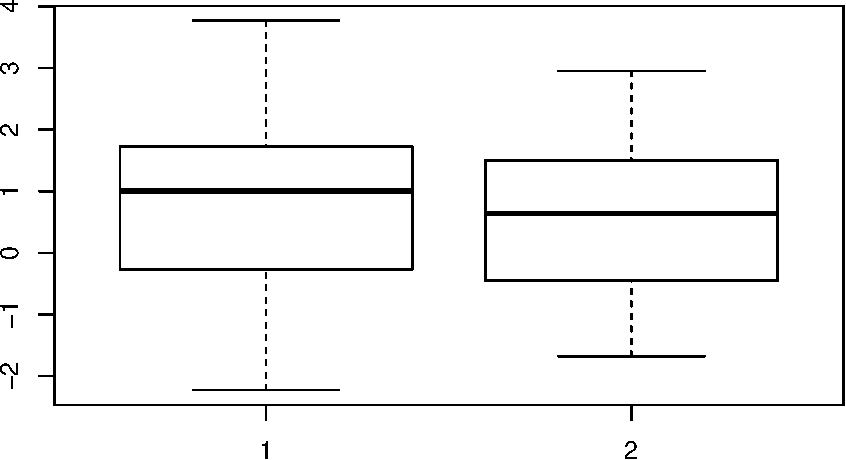
\includegraphics{prfe_files/figure-latex/unnamed-chunk-39-1.pdf}

We can add axis labels and a title to the graph:

\begin{Shaded}
\begin{Highlighting}[]
\KeywordTok{boxplot}\NormalTok{(WT }\OperatorTok{~}\StringTok{ }\NormalTok{LIFE,}
        \DataTypeTok{xlab =} \StringTok{"Life"}\NormalTok{,}
        \DataTypeTok{ylab =} \StringTok{"Weight"}\NormalTok{,}
        \DataTypeTok{main =} \StringTok{"Weight BY Life"}\NormalTok{)}
\end{Highlighting}
\end{Shaded}

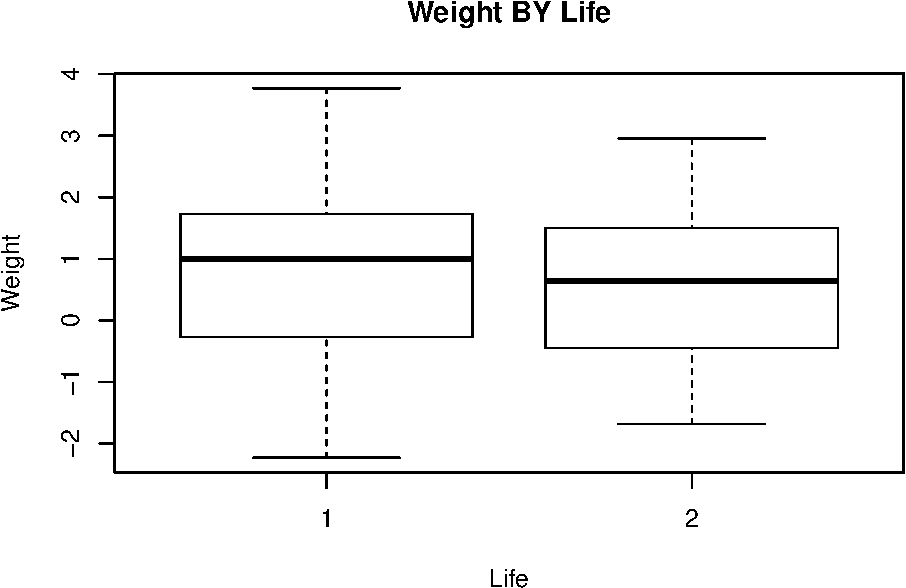
\includegraphics{prfe_files/figure-latex/unnamed-chunk-40-1.pdf}

A more descriptive title might be ``Weight Change BY Considered
Suicide''.

The groups do not seem to differ much in their medians and the
distributions appear to be reasonably symmetrical about their medians
with a similar spread of values.

We can look at the distribution as histograms:

\begin{Shaded}
\begin{Highlighting}[]
\KeywordTok{hist}\NormalTok{(WT[LIFE }\OperatorTok{==}\StringTok{ }\DecValTok{1}\NormalTok{])}
\end{Highlighting}
\end{Shaded}

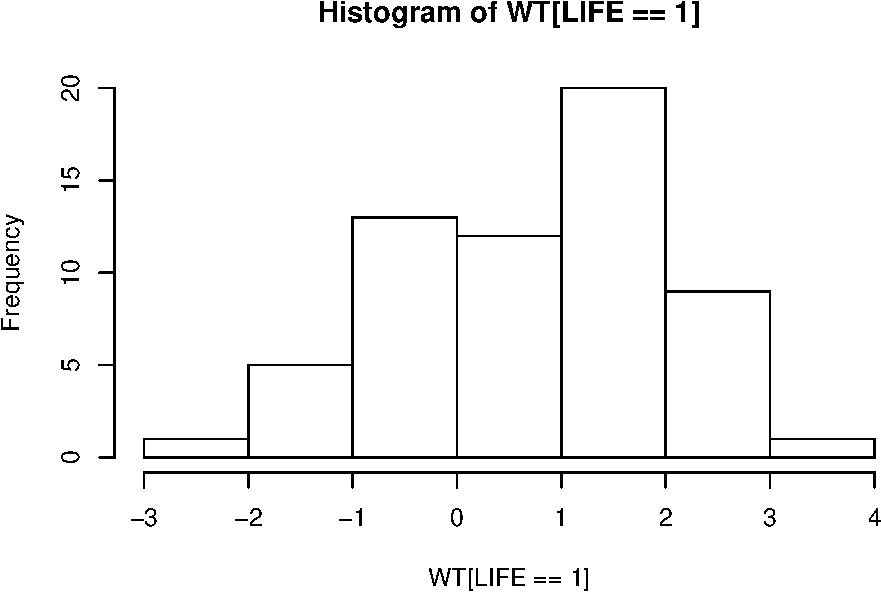
\includegraphics{prfe_files/figure-latex/unnamed-chunk-41-1.pdf}

\begin{Shaded}
\begin{Highlighting}[]
\KeywordTok{hist}\NormalTok{(WT[LIFE }\OperatorTok{==}\StringTok{ }\DecValTok{2}\NormalTok{])}
\end{Highlighting}
\end{Shaded}

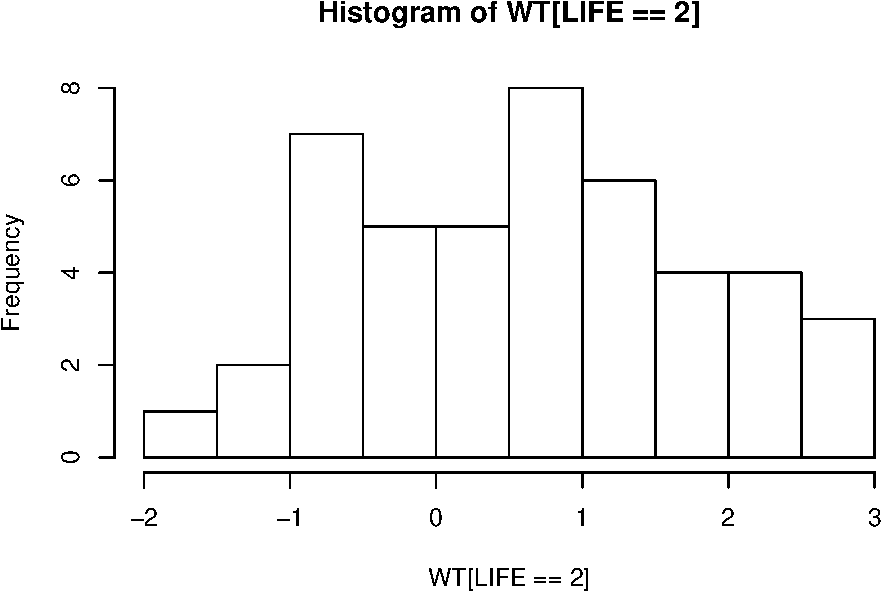
\includegraphics{prfe_files/figure-latex/unnamed-chunk-42-1.pdf}

and check the assumption of normality using quantile-quantile plots:

\begin{Shaded}
\begin{Highlighting}[]
\KeywordTok{qqnorm}\NormalTok{(WT[LIFE }\OperatorTok{==}\StringTok{ }\DecValTok{1}\NormalTok{])}
\KeywordTok{qqline}\NormalTok{(WT[LIFE }\OperatorTok{==}\StringTok{ }\DecValTok{1}\NormalTok{])}
\end{Highlighting}
\end{Shaded}

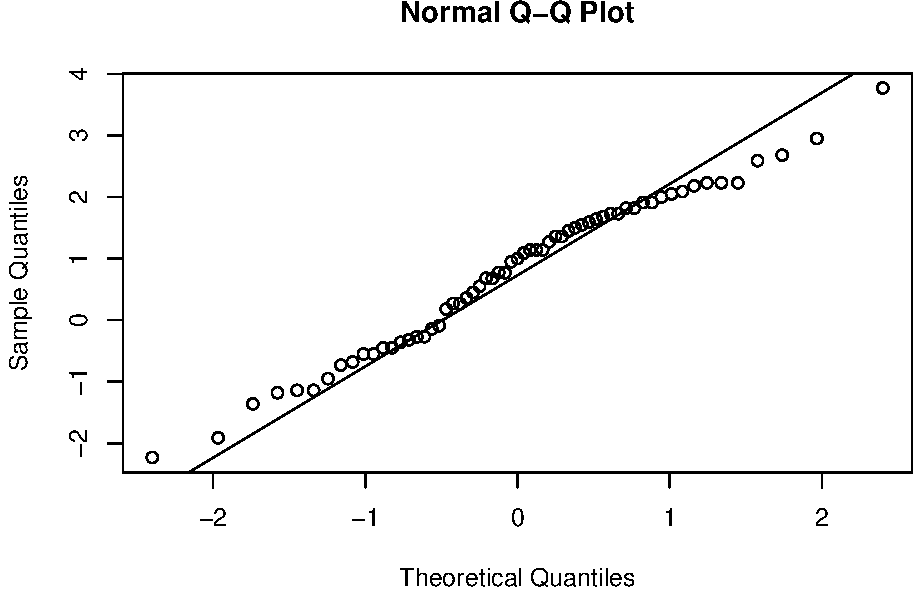
\includegraphics{prfe_files/figure-latex/unnamed-chunk-43-1.pdf}

\begin{Shaded}
\begin{Highlighting}[]
\KeywordTok{qqnorm}\NormalTok{(WT[LIFE }\OperatorTok{==}\StringTok{ }\DecValTok{2}\NormalTok{])}
\KeywordTok{qqline}\NormalTok{(WT[LIFE }\OperatorTok{==}\StringTok{ }\DecValTok{2}\NormalTok{])}
\end{Highlighting}
\end{Shaded}

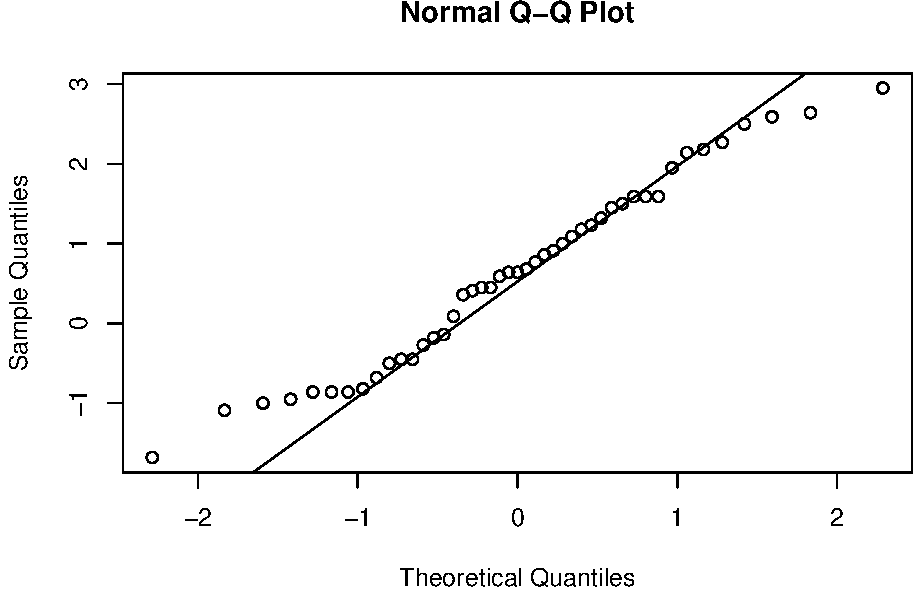
\includegraphics{prfe_files/figure-latex/unnamed-chunk-44-1.pdf}

or by using a formal test:

\begin{Shaded}
\begin{Highlighting}[]
\KeywordTok{shapiro.test}\NormalTok{(WT[LIFE }\OperatorTok{==}\StringTok{ }\DecValTok{1}\NormalTok{])}
\end{Highlighting}
\end{Shaded}

\begin{verbatim}
## 
##  Shapiro-Wilk normality test
## 
## data:  WT[LIFE == 1]
## W = 0.98038, p-value = 0.4336
\end{verbatim}

\begin{Shaded}
\begin{Highlighting}[]
\KeywordTok{shapiro.test}\NormalTok{(WT[LIFE }\OperatorTok{==}\StringTok{ }\DecValTok{2}\NormalTok{])}
\end{Highlighting}
\end{Shaded}

\begin{verbatim}
## 
##  Shapiro-Wilk normality test
## 
## data:  WT[LIFE == 2]
## W = 0.97155, p-value = 0.3292
\end{verbatim}

Remember that we can use the \texttt{by()} function to apply a function
to a data.frame, including statistical functions such as
\texttt{shapiro.test()}:

\begin{Shaded}
\begin{Highlighting}[]
\KeywordTok{by}\NormalTok{(WT, LIFE, shapiro.test)}
\end{Highlighting}
\end{Shaded}

\begin{verbatim}
## LIFE: 1
## 
##  Shapiro-Wilk normality test
## 
## data:  dd[x, ]
## W = 0.98038, p-value = 0.4336
## 
## -------------------------------------------------------- 
## LIFE: 2
## 
##  Shapiro-Wilk normality test
## 
## data:  dd[x, ]
## W = 0.97155, p-value = 0.3292
\end{verbatim}

We can also test whether the variances differ significantly using
\emph{Bartlett's test} for the homogeneity of variances:

\begin{Shaded}
\begin{Highlighting}[]
\KeywordTok{bartlett.test}\NormalTok{(WT, LIFE)}
\end{Highlighting}
\end{Shaded}

\begin{verbatim}
## 
##  Bartlett test of homogeneity of variances
## 
## data:  WT and LIFE
## Bartlett's K-squared = 0.32408, df = 1, p-value = 0.5692
\end{verbatim}

There is no significant difference between the two variances.

Many functions in \texttt{R} have a \emph{formula interface} that may be
used to specify multiple variables and the relations between multiple
variables. We could have used the formula interface with the
\texttt{bartlett.test()} function:

\begin{Shaded}
\begin{Highlighting}[]
\KeywordTok{bartlett.test}\NormalTok{(WT }\OperatorTok{~}\StringTok{ }\NormalTok{LIFE)}
\end{Highlighting}
\end{Shaded}

\begin{verbatim}
## 
##  Bartlett test of homogeneity of variances
## 
## data:  WT by LIFE
## Bartlett's K-squared = 0.32408, df = 1, p-value = 0.5692
\end{verbatim}

Having checked the normality and homogeneity of variance assumptions we
can proceed to carry out a \texttt{t-test}:

\begin{Shaded}
\begin{Highlighting}[]
\KeywordTok{t.test}\NormalTok{(WT }\OperatorTok{~}\StringTok{ }\NormalTok{LIFE, }\DataTypeTok{var.equal =} \OtherTok{TRUE}\NormalTok{)}
\end{Highlighting}
\end{Shaded}

\begin{verbatim}
## 
##  Two Sample t-test
## 
## data:  WT by LIFE
## t = 0.59869, df = 104, p-value = 0.5507
## alternative hypothesis: true difference in means is not equal to 0
## 95 percent confidence interval:
##  -0.3382365  0.6307902
## sample estimates:
## mean in group 1 mean in group 2 
##       0.7867213       0.6404444
\end{verbatim}

There is no evidence that the two groups differ in weight change in the
previous six months.

We could still have performed a \texttt{t-test} if the variances were
not homogenous by setting the \textbf{var.equal} parameter of the
\texttt{t.test()} function to \textbf{FALSE}:

\begin{Shaded}
\begin{Highlighting}[]
\KeywordTok{t.test}\NormalTok{(WT }\OperatorTok{~}\StringTok{ }\NormalTok{LIFE, }\DataTypeTok{var.equal =} \OtherTok{FALSE}\NormalTok{)}
\end{Highlighting}
\end{Shaded}

\begin{verbatim}
## 
##  Welch Two Sample t-test
## 
## data:  WT by LIFE
## t = 0.60608, df = 98.866, p-value = 0.5459
## alternative hypothesis: true difference in means is not equal to 0
## 95 percent confidence interval:
##  -0.3326225  0.6251763
## sample estimates:
## mean in group 1 mean in group 2 
##       0.7867213       0.6404444
\end{verbatim}

or performed a non-parametric test:

\begin{Shaded}
\begin{Highlighting}[]
\KeywordTok{wilcox.test}\NormalTok{(WT }\OperatorTok{~}\StringTok{ }\NormalTok{LIFE)}
\end{Highlighting}
\end{Shaded}

\begin{verbatim}
## 
##  Wilcoxon rank sum test with continuity correction
## 
## data:  WT by LIFE
## W = 1488, p-value = 0.4622
## alternative hypothesis: true location shift is not equal to 0
\end{verbatim}

An alternative, and more general, non-parametric test is:

\begin{Shaded}
\begin{Highlighting}[]
\KeywordTok{kruskal.test}\NormalTok{(WT }\OperatorTok{~}\StringTok{ }\NormalTok{LIFE)}
\end{Highlighting}
\end{Shaded}

\begin{verbatim}
## 
##  Kruskal-Wallis rank sum test
## 
## data:  WT by LIFE
## Kruskal-Wallis chi-squared = 0.54521, df = 1, p-value = 0.4603
\end{verbatim}

We can use the \texttt{table()} function to examine the differences in
depression between the two groups:

\begin{Shaded}
\begin{Highlighting}[]
\KeywordTok{table}\NormalTok{(DEP, LIFE)}
\end{Highlighting}
\end{Shaded}

\begin{verbatim}
##    LIFE
## DEP  1  2
##   1  0 26
##   2 42 24
##   3 16  1
\end{verbatim}

The two distributions look very different from each other. We can test
this using a chi-square test on the table:

\begin{Shaded}
\begin{Highlighting}[]
\KeywordTok{chisq.test}\NormalTok{(}\KeywordTok{table}\NormalTok{(DEP, LIFE))}
\end{Highlighting}
\end{Shaded}

\begin{verbatim}
## 
##  Pearson's Chi-squared test
## 
## data:  table(DEP, LIFE)
## X-squared = 43.876, df = 2, p-value = 2.968e-10
\end{verbatim}

Note that we passed the output of the \texttt{table()} function directly
to the \texttt{chisq.test()} function. We could have saved the table as
an object first and then passed the object to the \texttt{chisq.test()}
function:

\begin{Shaded}
\begin{Highlighting}[]
\NormalTok{tab <-}\StringTok{ }\KeywordTok{table}\NormalTok{(DEP, LIFE)}
\KeywordTok{chisq.test}\NormalTok{(tab)}
\end{Highlighting}
\end{Shaded}

\begin{verbatim}
## 
##  Pearson's Chi-squared test
## 
## data:  tab
## X-squared = 43.876, df = 2, p-value = 2.968e-10
\end{verbatim}

The \texttt{tab} object contains the output of the \texttt{table()}
function:

\begin{Shaded}
\begin{Highlighting}[]
\KeywordTok{class}\NormalTok{(tab)}
\end{Highlighting}
\end{Shaded}

\begin{verbatim}
## [1] "table"
\end{verbatim}

\begin{Shaded}
\begin{Highlighting}[]
\NormalTok{tab}
\end{Highlighting}
\end{Shaded}

\begin{verbatim}
##    LIFE
## DEP  1  2
##   1  0 26
##   2 42 24
##   3 16  1
\end{verbatim}

We can pass this table object to another function. For example:

\begin{Shaded}
\begin{Highlighting}[]
\KeywordTok{fisher.test}\NormalTok{(tab)}
\end{Highlighting}
\end{Shaded}

\begin{verbatim}
## 
##  Fisher's Exact Test for Count Data
## 
## data:  tab
## p-value = 1.316e-12
## alternative hypothesis: two.sided
\end{verbatim}

When we are finished with the tab object we can delete it using the
\texttt{rm()} function:

\begin{Shaded}
\begin{Highlighting}[]
\KeywordTok{rm}\NormalTok{(tab)}
\end{Highlighting}
\end{Shaded}

You can see a list of available objects using the \texttt{ls()}
function:

\begin{Shaded}
\begin{Highlighting}[]
\KeywordTok{ls}\NormalTok{()}
\end{Highlighting}
\end{Shaded}

\begin{verbatim}
## [1] "fem"
\end{verbatim}

This should just show the \texttt{fem} object.

We can examine the association between loss of interest in sex and
considering suicide in the same way:

\begin{Shaded}
\begin{Highlighting}[]
\NormalTok{tab <-}\StringTok{ }\KeywordTok{table}\NormalTok{(SEX, LIFE)}
\NormalTok{tab}
\end{Highlighting}
\end{Shaded}

\begin{verbatim}
##    LIFE
## SEX  1  2
##   1 58 38
##   2  5 12
\end{verbatim}

\begin{Shaded}
\begin{Highlighting}[]
\KeywordTok{fisher.test}\NormalTok{(tab)}
\end{Highlighting}
\end{Shaded}

\begin{verbatim}
## 
##  Fisher's Exact Test for Count Data
## 
## data:  tab
## p-value = 0.03175
## alternative hypothesis: true odds ratio is not equal to 1
## 95 percent confidence interval:
##   1.080298 14.214482
## sample estimates:
## odds ratio 
##   3.620646
\end{verbatim}

Note that with a two-by-two table the \texttt{fisher.test()} function
produces an estimate of, and confidence intervals for, the odds ratio.
Again, we will delete the \texttt{tab} object:

\begin{Shaded}
\begin{Highlighting}[]
\KeywordTok{rm}\NormalTok{(tab)}
\end{Highlighting}
\end{Shaded}

We could have performed the Fisher exact test without creating the tab
object by passing the output of the \texttt{table()} function directly
to the \texttt{fisher.test()} function:

\begin{Shaded}
\begin{Highlighting}[]
\KeywordTok{fisher.test}\NormalTok{(}\KeywordTok{table}\NormalTok{(SEX, LIFE))}
\end{Highlighting}
\end{Shaded}

\begin{verbatim}
## 
##  Fisher's Exact Test for Count Data
## 
## data:  table(SEX, LIFE)
## p-value = 0.03175
## alternative hypothesis: true odds ratio is not equal to 1
## 95 percent confidence interval:
##   1.080298 14.214482
## sample estimates:
## odds ratio 
##   3.620646
\end{verbatim}

Choose whichever method you find easiest but remember that it is easy to
save the results of any function for later use.

We can explore the correlation between two variables using the
\texttt{cor()} function:

\begin{Shaded}
\begin{Highlighting}[]
\KeywordTok{cor}\NormalTok{(IQ, WT, }\DataTypeTok{use =} \StringTok{"pairwise.complete.obs"}\NormalTok{)}
\end{Highlighting}
\end{Shaded}

\begin{verbatim}
## [1] -0.2917158
\end{verbatim}

or by using a scatter plot:

\begin{Shaded}
\begin{Highlighting}[]
\KeywordTok{plot}\NormalTok{(IQ, WT)}
\end{Highlighting}
\end{Shaded}

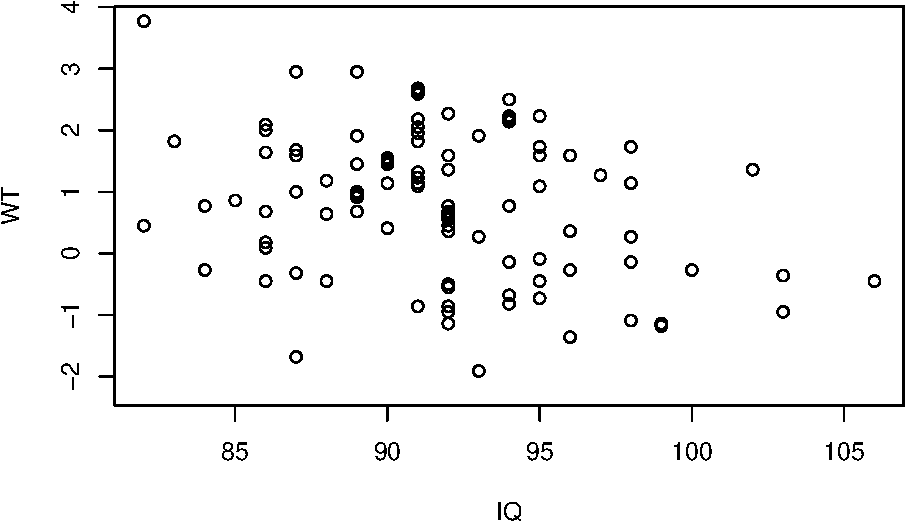
\includegraphics{prfe_files/figure-latex/unnamed-chunk-64-1.pdf}

and by a formal test:

\begin{Shaded}
\begin{Highlighting}[]
\KeywordTok{cor.test}\NormalTok{(IQ, WT)}
\end{Highlighting}
\end{Shaded}

\begin{verbatim}
## 
##  Pearson's product-moment correlation
## 
## data:  IQ and WT
## t = -3.0192, df = 98, p-value = 0.003231
## alternative hypothesis: true correlation is not equal to 0
## 95 percent confidence interval:
##  -0.4616804 -0.1010899
## sample estimates:
##        cor 
## -0.2917158
\end{verbatim}

With some functions you can pass an entire data.frame rather than a list
of variables:

\begin{Shaded}
\begin{Highlighting}[]
\KeywordTok{cor}\NormalTok{(fem, }\DataTypeTok{use =} \StringTok{"pairwise.complete.obs"}\NormalTok{)}
\end{Highlighting}
\end{Shaded}

\begin{verbatim}
##               ID         AGE            IQ         ANX           DEP
## ID    1.00000000  0.03069077  0.0370598672 -0.02941825 -0.0554147209
## AGE   0.03069077  1.00000000 -0.4345435680  0.06734300 -0.0387049246
## IQ    0.03705987 -0.43454357  1.0000000000 -0.02323787 -0.0001307404
## ANX  -0.02941825  0.06734300 -0.0232378691  1.00000000  0.5437946347
## DEP  -0.05541472 -0.03870492 -0.0001307404  0.54379463  1.0000000000
## SLP  -0.07268743  0.02606547  0.0812993104  0.22317875  0.5248724551
## SEX   0.08999634  0.10609216 -0.0536558660 -0.21062493 -0.3058422258
## LIFE -0.05604349 -0.10300193 -0.0915396469 -0.34211268 -0.6139017253
## WT    0.02640131  0.41574411 -0.2917157832  0.11817532  0.0233742465
##               SLP         SEX        LIFE           WT
## ID   -0.072687434  0.08999634 -0.05604349  0.026401310
## AGE   0.026065468  0.10609216 -0.10300193  0.415744109
## IQ    0.081299310 -0.05365587 -0.09153965 -0.291715783
## ANX   0.223178752 -0.21062493 -0.34211268  0.118175321
## DEP   0.524872455 -0.30584223 -0.61390173  0.023374247
## SLP   1.000000000 -0.29053971 -0.35186578 -0.009259774
## SEX  -0.290539709  1.00000000  0.22316967 -0.027826514
## LIFE -0.351865775  0.22316967  1.00000000 -0.058605326
## WT   -0.009259774 -0.02782651 -0.05860533  1.000000000
\end{verbatim}

\begin{Shaded}
\begin{Highlighting}[]
\KeywordTok{pairs}\NormalTok{(fem)}
\end{Highlighting}
\end{Shaded}

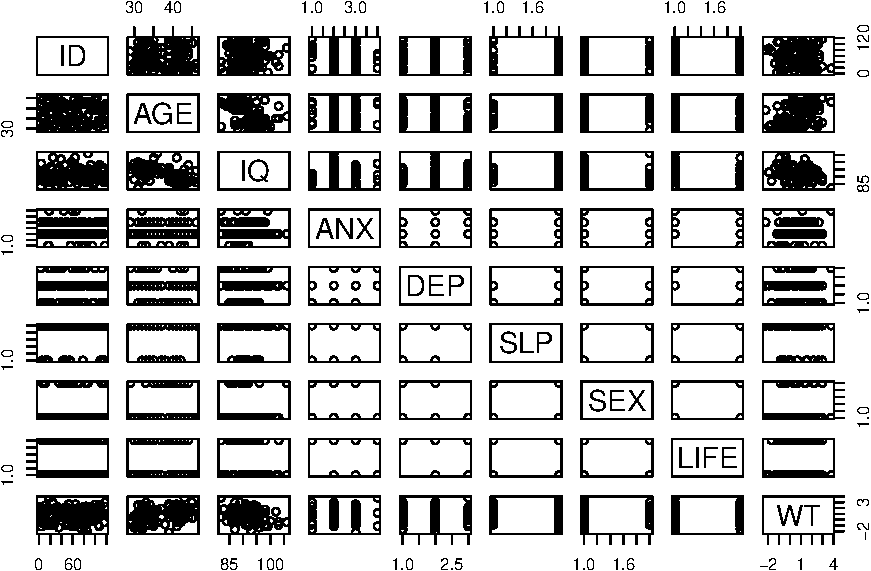
\includegraphics{prfe_files/figure-latex/unnamed-chunk-66-1.pdf}

The output can be a little confusing particularly if it includes
categorical or record identifying variables. To avoid this we can create
a new object that contains only the columns we are interested in using
the column binding \texttt{cbind()} function:

\begin{Shaded}
\begin{Highlighting}[]
\NormalTok{newfem <-}\StringTok{ }\KeywordTok{cbind}\NormalTok{(AGE, IQ, WT)}
\KeywordTok{cor}\NormalTok{(newfem, }\DataTypeTok{use =} \StringTok{"pairwise.complete.obs"}\NormalTok{)}
\end{Highlighting}
\end{Shaded}

\begin{verbatim}
##            AGE         IQ         WT
## AGE  1.0000000 -0.4345436  0.4157441
## IQ  -0.4345436  1.0000000 -0.2917158
## WT   0.4157441 -0.2917158  1.0000000
\end{verbatim}

\begin{Shaded}
\begin{Highlighting}[]
\KeywordTok{pairs}\NormalTok{(newfem)}
\end{Highlighting}
\end{Shaded}

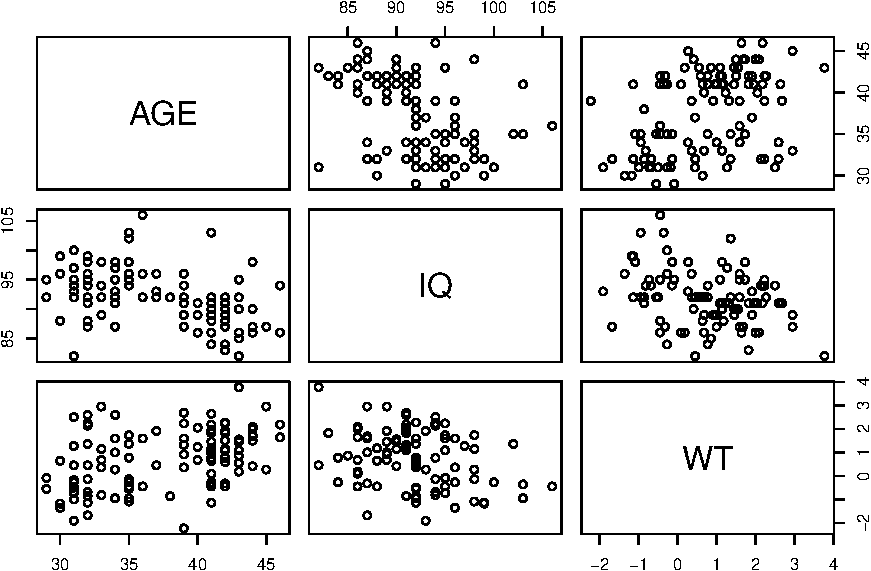
\includegraphics{prfe_files/figure-latex/unnamed-chunk-67-1.pdf}

When we have finished with the \texttt{newfem} object we can delete it:

\begin{Shaded}
\begin{Highlighting}[]
\KeywordTok{rm}\NormalTok{(newfem)}
\end{Highlighting}
\end{Shaded}

There was no real need to create the \texttt{newfem} object as we could
have fed the output of the \texttt{cbind()} function directly to the
\texttt{cor()} or \texttt{pairs()} function:

\begin{Shaded}
\begin{Highlighting}[]
\KeywordTok{cor}\NormalTok{(}\KeywordTok{cbind}\NormalTok{(AGE, IQ, WT), }\DataTypeTok{use =} \StringTok{"pairwise.complete.obs"}\NormalTok{)}
\end{Highlighting}
\end{Shaded}

\begin{verbatim}
##            AGE         IQ         WT
## AGE  1.0000000 -0.4345436  0.4157441
## IQ  -0.4345436  1.0000000 -0.2917158
## WT   0.4157441 -0.2917158  1.0000000
\end{verbatim}

\begin{Shaded}
\begin{Highlighting}[]
\KeywordTok{pairs}\NormalTok{(}\KeywordTok{cbind}\NormalTok{(AGE, IQ, WT))}
\end{Highlighting}
\end{Shaded}

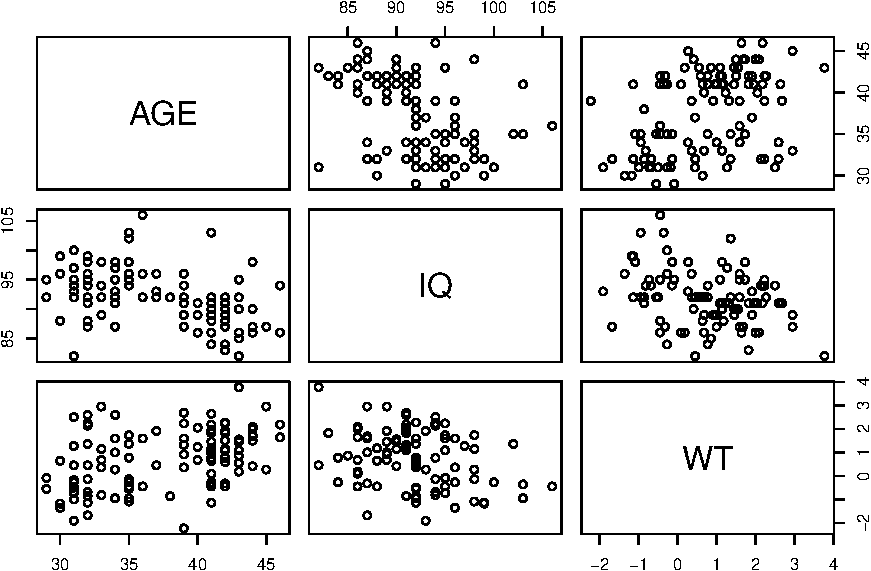
\includegraphics{prfe_files/figure-latex/unnamed-chunk-69-1.pdf}

It is, however, easier to work with the \texttt{newfem} object rather
than having to retype the \texttt{cbind()} function. This is
particularly true if you wanted to continue with an analysis of just the
three variables.

The relationship between \texttt{AGE} and \texttt{WT} can be plotted
using the \texttt{plot()} function:

\begin{Shaded}
\begin{Highlighting}[]
\KeywordTok{plot}\NormalTok{(AGE, WT)}
\end{Highlighting}
\end{Shaded}

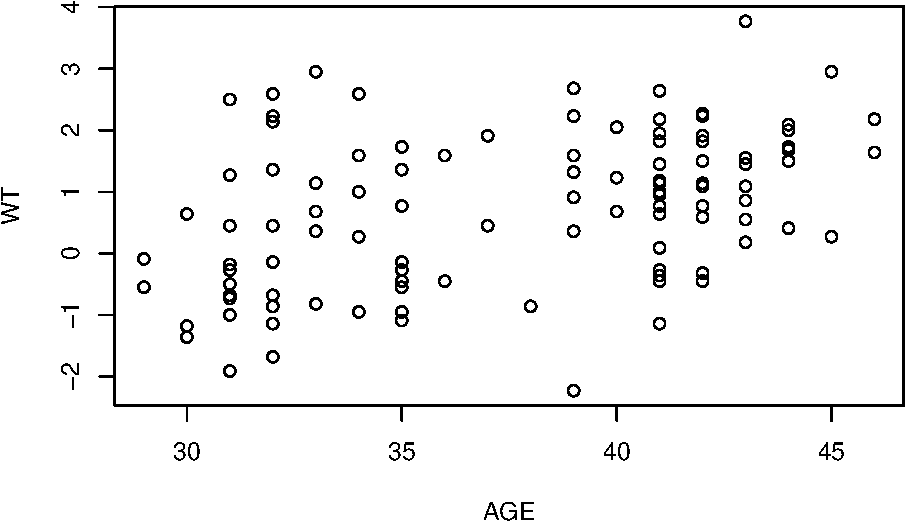
\includegraphics{prfe_files/figure-latex/unnamed-chunk-70-1.pdf}

And tested using the \texttt{cor()} and \texttt{cor.test()} functions:

\begin{Shaded}
\begin{Highlighting}[]
\KeywordTok{cor}\NormalTok{(AGE, WT, }\DataTypeTok{use =} \StringTok{"pairwise.complete.obs"}\NormalTok{)}
\end{Highlighting}
\end{Shaded}

\begin{verbatim}
## [1] 0.4157441
\end{verbatim}

\begin{Shaded}
\begin{Highlighting}[]
\KeywordTok{cor.test}\NormalTok{(AGE, WT)}
\end{Highlighting}
\end{Shaded}

\begin{verbatim}
## 
##  Pearson's product-moment correlation
## 
## data:  AGE and WT
## t = 4.6841, df = 105, p-value = 8.457e-06
## alternative hypothesis: true correlation is not equal to 0
## 95 percent confidence interval:
##  0.2452434 0.5612979
## sample estimates:
##       cor 
## 0.4157441
\end{verbatim}

Or by using the linear modelling \texttt{lm()} function:

\begin{Shaded}
\begin{Highlighting}[]
\KeywordTok{summary}\NormalTok{(}\KeywordTok{lm}\NormalTok{(WT }\OperatorTok{~}\StringTok{ }\NormalTok{AGE))}
\end{Highlighting}
\end{Shaded}

\begin{verbatim}
## 
## Call:
## lm(formula = WT ~ AGE)
## 
## Residuals:
##      Min       1Q   Median       3Q      Max 
## -3.10678 -0.85922 -0.05453  0.71434  2.70874 
## 
## Coefficients:
##             Estimate Std. Error t value Pr(>|t|)    
## (Intercept) -3.25405    0.85547  -3.804  0.00024 ***
## AGE          0.10592    0.02261   4.684 8.46e-06 ***
## ---
## Signif. codes:  0 '***' 0.001 '**' 0.01 '*' 0.05 '.' 0.1 ' ' 1
## 
## Residual standard error: 1.128 on 105 degrees of freedom
##   (11 observations deleted due to missingness)
## Multiple R-squared:  0.1728, Adjusted R-squared:  0.165 
## F-statistic: 21.94 on 1 and 105 DF,  p-value: 8.457e-06
\end{verbatim}

We use the \texttt{summary()} function here to extract summary
information from the output of the \texttt{lm()} function.

It is often more useful to use \texttt{lm()} to create an object:

\begin{Shaded}
\begin{Highlighting}[]
\NormalTok{fem.lm <-}\StringTok{ }\KeywordTok{lm}\NormalTok{(WT }\OperatorTok{~}\StringTok{ }\NormalTok{AGE)}
\end{Highlighting}
\end{Shaded}

And use the output in other functions:

\begin{Shaded}
\begin{Highlighting}[]
\KeywordTok{summary}\NormalTok{(fem.lm)}
\end{Highlighting}
\end{Shaded}

\begin{verbatim}
## 
## Call:
## lm(formula = WT ~ AGE)
## 
## Residuals:
##      Min       1Q   Median       3Q      Max 
## -3.10678 -0.85922 -0.05453  0.71434  2.70874 
## 
## Coefficients:
##             Estimate Std. Error t value Pr(>|t|)    
## (Intercept) -3.25405    0.85547  -3.804  0.00024 ***
## AGE          0.10592    0.02261   4.684 8.46e-06 ***
## ---
## Signif. codes:  0 '***' 0.001 '**' 0.01 '*' 0.05 '.' 0.1 ' ' 1
## 
## Residual standard error: 1.128 on 105 degrees of freedom
##   (11 observations deleted due to missingness)
## Multiple R-squared:  0.1728, Adjusted R-squared:  0.165 
## F-statistic: 21.94 on 1 and 105 DF,  p-value: 8.457e-06
\end{verbatim}

\begin{Shaded}
\begin{Highlighting}[]
\KeywordTok{plot}\NormalTok{(AGE, WT)}
\KeywordTok{abline}\NormalTok{(fem.lm)}
\end{Highlighting}
\end{Shaded}

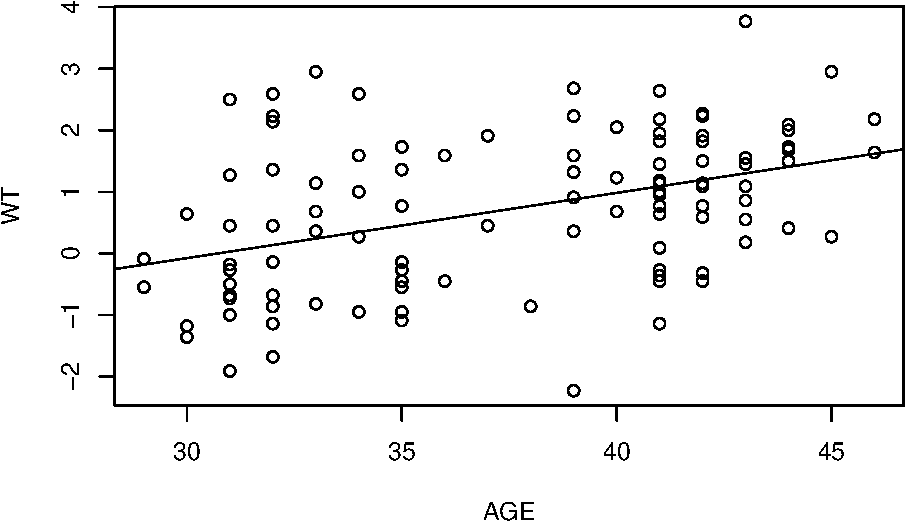
\includegraphics{prfe_files/figure-latex/unnamed-chunk-74-1.pdf}

In this case we are passing the intercept and slope information held in
the \texttt{fem.lm} object to the \texttt{abline()} function which draws
a regression line. The \texttt{abline()} function adds to an existing
plot. This means that you need to keep the scatter plot of \texttt{AGE}
and \texttt{WT} open before issuing the \texttt{abline()} function call.

A useful function to apply to the \texttt{fem.lm} object is
\texttt{plot()} which produces diagnostic plots of the linear model:

\begin{Shaded}
\begin{Highlighting}[]
\KeywordTok{plot}\NormalTok{(fem.lm)}
\end{Highlighting}
\end{Shaded}

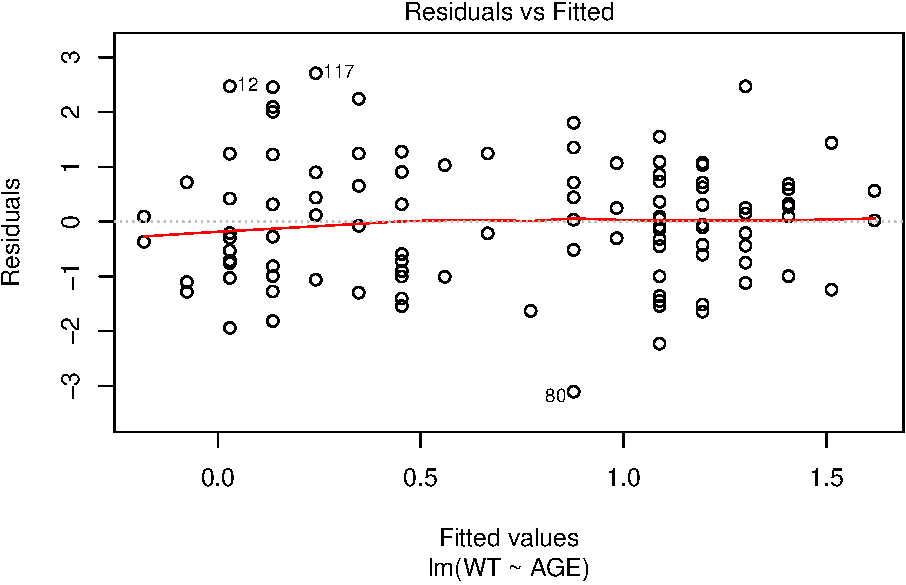
\includegraphics{prfe_files/figure-latex/unnamed-chunk-75-1.pdf}
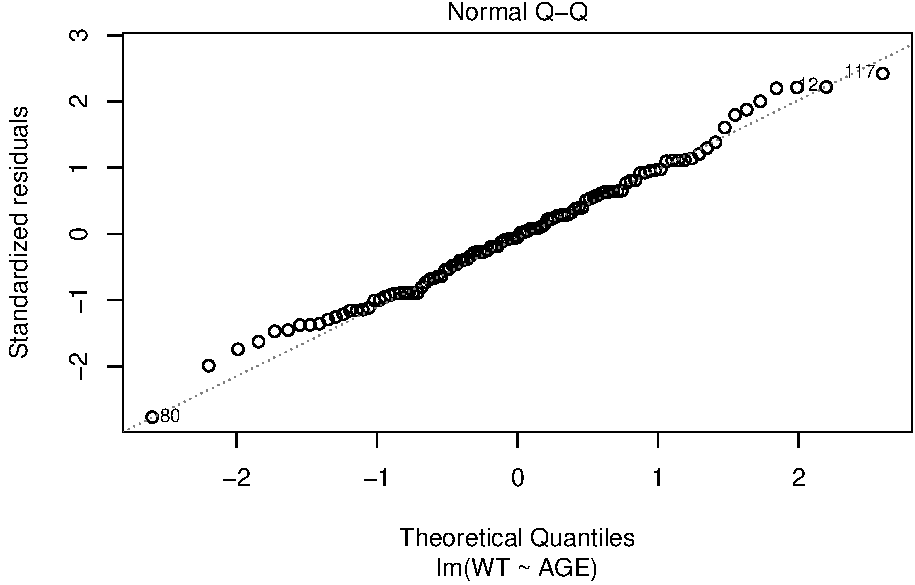
\includegraphics{prfe_files/figure-latex/unnamed-chunk-75-2.pdf}
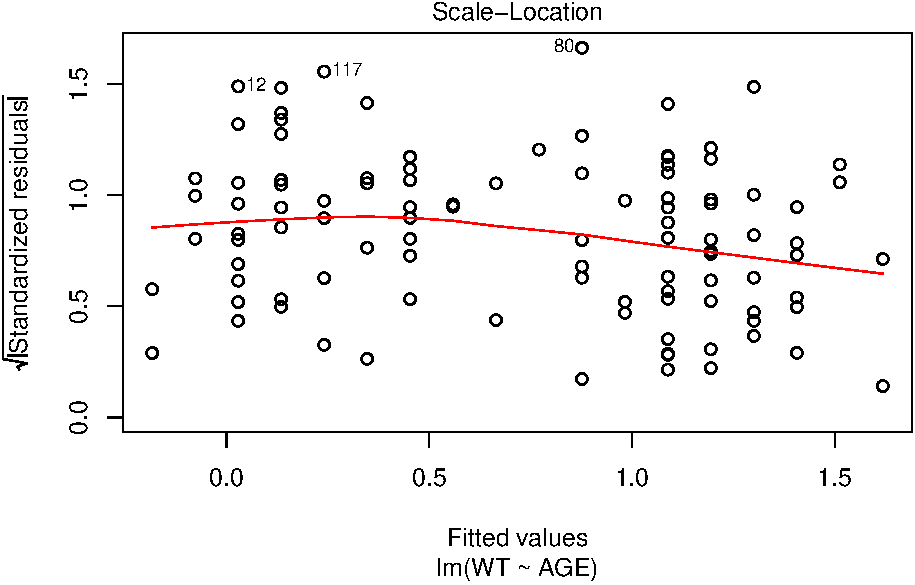
\includegraphics{prfe_files/figure-latex/unnamed-chunk-75-3.pdf}
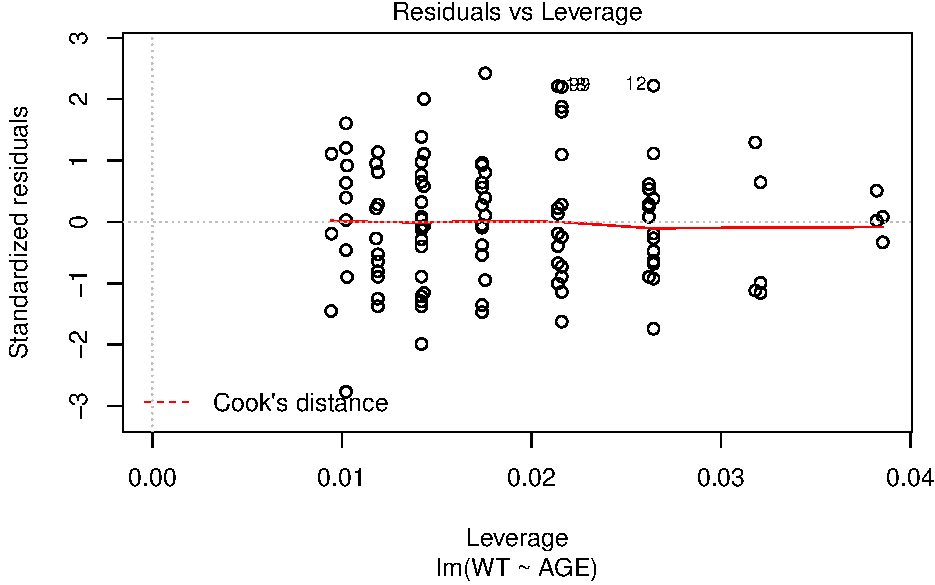
\includegraphics{prfe_files/figure-latex/unnamed-chunk-75-4.pdf}

Objects created by the \texttt{lm()} function (or any of the modelling
functions) can use up a lot of memory so we should remove them when we
no longer need them:

\begin{Shaded}
\begin{Highlighting}[]
\KeywordTok{rm}\NormalTok{(fem.lm)}
\end{Highlighting}
\end{Shaded}

It might be interesting to see whether a similar relationship exists
between \texttt{AGE} and \texttt{WT} for those who have and have not
considered suicide. This can be done using the \texttt{coplot()}
function:

\begin{Shaded}
\begin{Highlighting}[]
\KeywordTok{coplot}\NormalTok{(WT }\OperatorTok{~}\StringTok{ }\NormalTok{AGE }\OperatorTok{|}\StringTok{ }\KeywordTok{as.factor}\NormalTok{(LIFE))}
\end{Highlighting}
\end{Shaded}

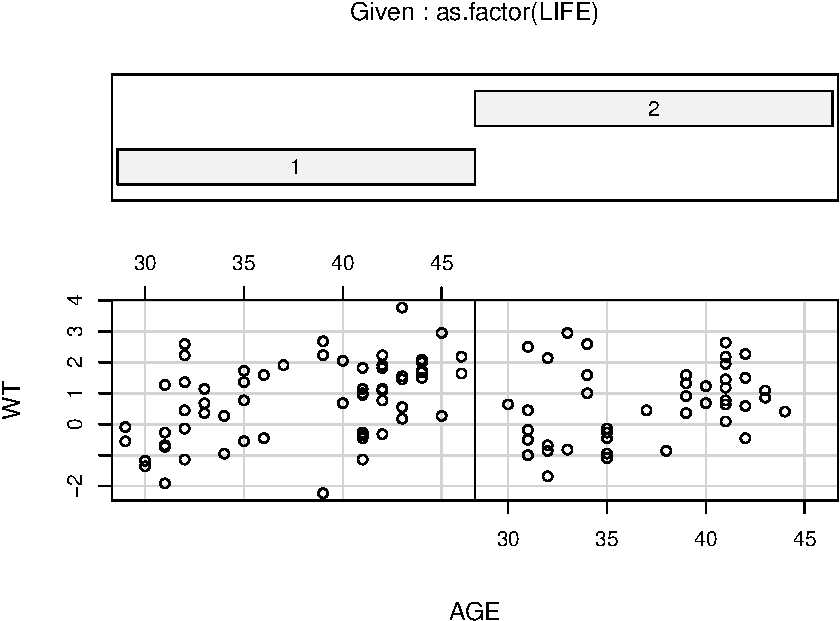
\includegraphics{prfe_files/figure-latex/unnamed-chunk-77-1.pdf}

\begin{verbatim}
## 
##  Missing rows: 21, 22, 31, 43, 44, 45, 69, 81, 101, 104, 114, 115
\end{verbatim}

The two plots looks similar. We could also use \texttt{coplot()} to
investigate the relationship between \texttt{AGE} and \texttt{WT} for
categories of both \texttt{LIFE} and \texttt{SEX}:

\begin{Shaded}
\begin{Highlighting}[]
\KeywordTok{coplot}\NormalTok{(WT }\OperatorTok{~}\StringTok{ }\NormalTok{AGE }\OperatorTok{|}\StringTok{ }\KeywordTok{as.factor}\NormalTok{(LIFE) }\OperatorTok{*}\StringTok{ }\KeywordTok{as.factor}\NormalTok{(SEX))}
\end{Highlighting}
\end{Shaded}

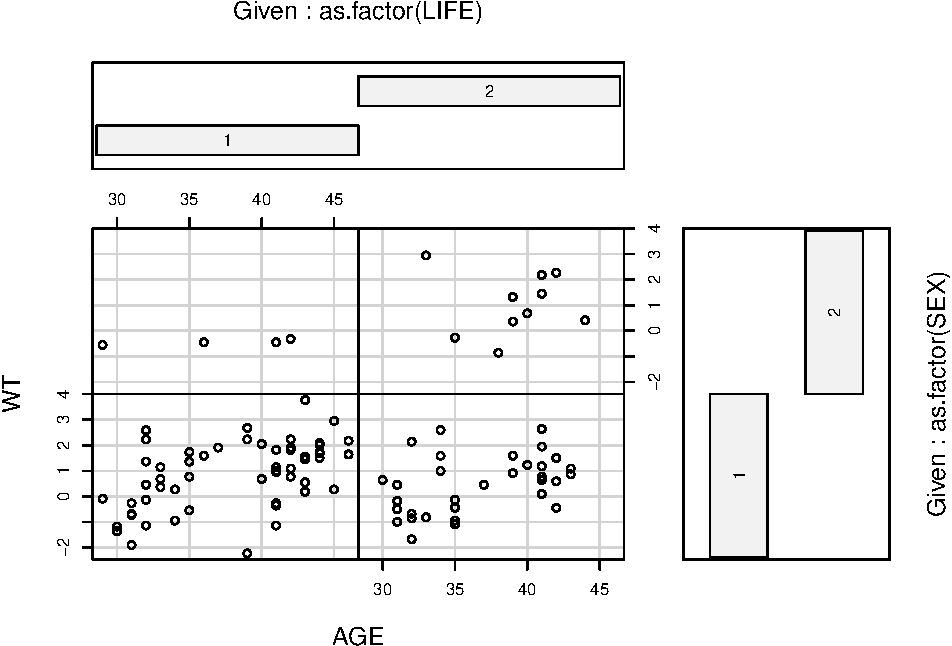
\includegraphics{prfe_files/figure-latex/unnamed-chunk-78-1.pdf}

\begin{verbatim}
## 
##  Missing rows: 12, 17, 21, 22, 31, 43, 44, 45, 66, 69, 81, 101, 104, 105, 114, 115
\end{verbatim}

although the numbers are too small for this to be useful here.

We used the \texttt{as.factor()} function with the \texttt{coplot()}
function to ensure that \texttt{R} was aware that the \texttt{LIFE} and
\texttt{SEX} columns hold categorical data.

We can check the way variables are stored using the
\texttt{data.class()} function:

\begin{Shaded}
\begin{Highlighting}[]
\KeywordTok{data.class}\NormalTok{(fem}\OperatorTok{$}\NormalTok{SEX)}
\end{Highlighting}
\end{Shaded}

\begin{verbatim}
## [1] "numeric"
\end{verbatim}

We can `apply' this function to all columns in a data.frame using the
\texttt{sapply()} function:

\begin{Shaded}
\begin{Highlighting}[]
\KeywordTok{sapply}\NormalTok{(fem, data.class)}
\end{Highlighting}
\end{Shaded}

\begin{verbatim}
##        ID       AGE        IQ       ANX       DEP       SLP       SEX 
## "numeric" "numeric" "numeric" "numeric" "numeric" "numeric" "numeric" 
##      LIFE        WT 
## "numeric" "numeric"
\end{verbatim}

The \texttt{sapply()} function is part of a group of functions that
apply a specified function to data objects:

\begin{longtable}[]{@{}ll@{}}
\toprule
\begin{minipage}[b]{0.27\columnwidth}\raggedright
\textbf{Function(s)}\strut
\end{minipage} & \begin{minipage}[b]{0.67\columnwidth}\raggedright
\textbf{Applies a function to \ldots{}}\strut
\end{minipage}\tabularnewline
\midrule
\endhead
\begin{minipage}[t]{0.27\columnwidth}\raggedright
\texttt{apply()}\strut
\end{minipage} & \begin{minipage}[t]{0.67\columnwidth}\raggedright
rows and columns of matrices, arrays, and tables\strut
\end{minipage}\tabularnewline
\begin{minipage}[t]{0.27\columnwidth}\raggedright
\texttt{lapply()}\strut
\end{minipage} & \begin{minipage}[t]{0.67\columnwidth}\raggedright
components of lists and data.frames\strut
\end{minipage}\tabularnewline
\begin{minipage}[t]{0.27\columnwidth}\raggedright
\texttt{sapply()}\strut
\end{minipage} & \begin{minipage}[t]{0.67\columnwidth}\raggedright
components of lists and data.frames\strut
\end{minipage}\tabularnewline
\begin{minipage}[t]{0.27\columnwidth}\raggedright
\texttt{mapply()}\strut
\end{minipage} & \begin{minipage}[t]{0.67\columnwidth}\raggedright
components of lists and data.frames\strut
\end{minipage}\tabularnewline
\begin{minipage}[t]{0.27\columnwidth}\raggedright
\texttt{tapply()}\strut
\end{minipage} & \begin{minipage}[t]{0.67\columnwidth}\raggedright
subsets of data\strut
\end{minipage}\tabularnewline
\bottomrule
\end{longtable}

Related functions are \texttt{aggregate()} which compute summary
statistics for subsets of data, \texttt{by()} which applies a function
to a data.frame split by factors, and \texttt{sweep()} which applies a
function to an array.

The parameters of most \texttt{R} functions have default values. These
are usually the most used and most useful parameter values for each
function. The \texttt{cor.test()} function, for example, calculates
\emph{Pearson's product moment correlation coefficient} by default. This
is an appropriate measure for data from a bivariate normal distribution.
The \texttt{DEP} and \texttt{ANX} variables contain ordered data. An
appropriate measure of correlation between \texttt{DEP} and \texttt{ANX}
is \emph{Kendall's tau}. This can be obtained using:

\begin{Shaded}
\begin{Highlighting}[]
\KeywordTok{cor.test}\NormalTok{(DEP, ANX, }\DataTypeTok{method =} \StringTok{"kendall"}\NormalTok{)}
\end{Highlighting}
\end{Shaded}

\begin{verbatim}
## 
##  Kendall's rank correlation tau
## 
## data:  DEP and ANX
## z = 5.5606, p-value = 2.689e-08
## alternative hypothesis: true tau is not equal to 0
## sample estimates:
##       tau 
## 0.4950723
\end{verbatim}

Before we finish we should save the \texttt{fem} data.frame so that next
time we want to use it we will not have to bother with recoding the
missing values to the special \texttt{NA} value. This is done with the
\texttt{write.table()} function:

\begin{Shaded}
\begin{Highlighting}[]
\KeywordTok{write.table}\NormalTok{(fem, }\DataTypeTok{file =} \StringTok{"newfem.dat"}\NormalTok{, }\DataTypeTok{row.names =} \OtherTok{FALSE}\NormalTok{)}
\end{Highlighting}
\end{Shaded}

Everything in \texttt{R} is either a function or an object. Even the
command to quit \texttt{R} is a function:

\begin{Shaded}
\begin{Highlighting}[]
\KeywordTok{q}\NormalTok{()}
\end{Highlighting}
\end{Shaded}

When you call the \texttt{q()} function you will be asked if you want to
save the workspace image. If you save the workspace image then all of
the objects and functions currently available to you will be saved.
These will then be automatically restored the next time you start
\texttt{R} in the current working directory.

For this exercise there is no need to save the workspace image so click
the \textbf{No} or \textbf{Don't Save} button (GUI) or enter \texttt{n}
when prompted to save the workspace image (terminal).

\hypertarget{summary}{%
\section{Summary}\label{summary}}

\begin{itemize}
\tightlist
\item
  \texttt{R} is a functional system. Everything is done by calling
  functions.
\item
  \texttt{R} provides a large set of functions for descriptive
  statistics, charting, and statistical inference.
\item
  Functions can be chained together so that the output of one function
  is the input of another function.
\item
  \texttt{R} is an object oriented system. We can use functions to
  create objects that can then be manipulated or passed to other
  functions for subsequent analysis.
\end{itemize}

\hypertarget{exercise2}{%
\chapter{Manipulating objects and creating new
functions}\label{exercise2}}

In this exercise we will explore how to manipulate \texttt{R} objects
and how to write functions that can manipulate and extract data and
information from \texttt{R} objects and produce useful analyses.

Before we go any further we should start \texttt{R} and retrieve a
dataset:

\begin{Shaded}
\begin{Highlighting}[]
\NormalTok{salex <-}\StringTok{ }\KeywordTok{read.table}\NormalTok{(}\StringTok{"salex.dat"}\NormalTok{, }\DataTypeTok{header =} \OtherTok{TRUE}\NormalTok{, }\DataTypeTok{na.strings =} \StringTok{"9"}\NormalTok{)}
\end{Highlighting}
\end{Shaded}

Missing values are coded as 9 throughout this dataset so we can use the
\texttt{na.strings} parameter of the \texttt{read.table()} function to
replace all 9's with the special \texttt{NA} code when we retrieve the
dataset. Check that this works by examining the \texttt{salex}
data.frame:

\begin{Shaded}
\begin{Highlighting}[]
\NormalTok{salex}
\end{Highlighting}
\end{Shaded}

\begin{verbatim}
##    ILL HAM BEEF EGGS MUSHROOM PEPPER PORKPIE PASTA RICE LETTUCE TOMATO
## 1    1   1    1    1        1      1       2     2    2       2      2
## 2    1   1    1    1        2      2       1     2    2       2      1
## 3    1   1    1    1        1      1       1     1    1       1      2
## 4    1   1    1    1        2      2       2     2    2       1      1
## 5    1   1    1    1        1      1       1     1    1       1      1
## 6    1   1    1    1        2      2       2     2    2       2      1
## 7    1   1    1    1        1      1       1     2    2       2      2
## 8    1   1    2    1        1      1       2     1    1       1      2
## 9    1   1    1    1        2      1       1     2    1       2      2
## 10   1   1    1    1        2      1       1     1    1       1      1
## 11   1   2    2    1        1      1       2     2    2       1      1
## 12   1   1    1    1        2      2       2     2    2       2      2
## 13   2   2    1    2        2      2       1     2    2       2      1
## 14   1   1    1    1        2      2       2     1    1       2      1
## 15   1   1    1    1        1      1       2     1    1       2      2
## 16   1   1    1    1        1      1       1     2    2       2      2
## 17   1   1    1    1        1      1       1     1    1       1      1
## 18   2   1    1    2        2      2       2     2    2       2      2
## 19   2   1    1    1        1      2       2     1    1       2      1
## 20   2   1    1    2        2      2       2     2    2       2      2
## 21   2   2    2    2        2      2       2     2    2       2      2
## 22   1   1    1    1        2      2       2     2    2       1      1
## 23   1   2    1    2        2      2       2     1    1       2      1
## 24   1   1    1    1        2      1       2     1    1       2      2
## 25   1   1    1    2        1      1       1     1    1       1      1
## 26   1   1    2    1        1      1       2     2    2       1      1
## 27   1   1    1    1        2      2       1     2    1       1      1
## 28   1   1    1    1        1      1       2     1    1       2      2
## 29   1   2    1    1        1     NA       2     1    1       1      1
## 30   1   1    1    2        2      2       1     2    2       2      2
## 31   1   1    1    1        1      2       2     1    1       2      2
## 32   1   1    1    1        1      2      NA     2    1       1      1
## 33   1   1    1    1        2      2       2     1    2       2      2
## 34   1   1    1    1        1      2       2     2    2       1      1
## 35   1   1    1    1        1      1       1     1    2       2      1
## 36   2   2    1    2        2      2       2     2    2       2      2
## 37   1   1    1    1        1      1       2     1    1       1      1
## 38   1   1    1    2        2      2       1     1    1       1      2
## 39   1   1    1    1        1      1       1     2    2       1      2
## 40   1   1    1    1        1      1       1     2    2       1      1
## 41   1   1    1    2        2      1       2     1    1       1      1
## 42   1   1    1    2        2      2       2     2    2       2      2
## 43   1   1    1    1        1      1       2     1    1       1      1
## 44   1   2    1    2        2      2       1     2    2       1      2
## 45   1   1    1    1        1      2       2     2    1       1      1
## 46   1   1    1    2        2      2       2     1    1       1      1
## 47   1   1    1    1        2      2       2     2    1       1      2
## 48   1   1    1    1        1     NA       1     1    1       2      2
## 49   1   1    1    1        2      1       2     2    1       1      1
## 50   1   2    1    1        2      2       2     1    2       2      1
## 51   2   2    1    2        2      2       2     2    2       2      2
## 52   2   1    1    2        2      2       2     1    2       2      1
## 53   2   1    1    2        2      2       1     2    2       2      1
## 54   2   1    1    2        1      2       1     2    2       2      1
## 55   2   1    1    1        1      1       2     2    1       2      2
## 56   2   1    1    2        2      2       2     2    2       2      1
## 57   2   1    1    1        1      1       1     2    2       2      2
## 58   2   1    1    1        2      2       1     2    1       2      2
## 59   2   1    1    2        2      2       2     2    2       2      2
## 60   2   2    2    2        2      2       1     2    2       2      2
## 61   2   1    1    2        2      2       1     2    2       2      2
## 62   2   1    2    2        2      2       2     2    2       1      1
## 63   1   1    1    1        1      1       2     2    2       2      1
## 64   2   1    1    2        2      2       2     2    2       2      2
## 65   2   1    1    1        1      2       1     2    1       2      2
## 66   2   2    1    2        2      2       2     2    2       2      2
## 67   2   2    1    2        2      2       2     2    2       2      2
## 68   2   1    1    2        1      1       1     1    2       2      1
## 69   2   2    1    2        2      2       2     2    2       2      2
## 70   2   2    1    2        2      2       2     2    2       2      2
## 71   1   1    2    2        2      2       1     2    1       2      2
## 72   2   1    2    1       NA     NA       2     2    2       2      1
## 73   1   1    1    1        2      2       1     2    2       2      2
## 74   1   1    2    1       NA     NA       2     1    1       1      1
## 75   1   1    2    2        2      1       2     1    2       1      1
## 76   1   1    1    1        2      2       1     1    2       2      2
## 77   1   1    1   NA       NA     NA       1     2    1       1      1
##    COLESLAW CRISPS PEACHCAKE CHOCOLATE FRUIT TRIFLE ALMONDS
## 1         2      2         2         2     2      2       2
## 2         2      2         2         2     2      2       2
## 3         2      1         2         1     2      2       2
## 4         2      2         2         1     2      2       2
## 5         1      2         2         1     2      1       2
## 6         1      1         2         1     2      2       2
## 7         1      1         1         2     2      2       2
## 8         1      1         2         2     2      1       2
## 9         2      2         2         2     2      1       2
## 10        1      1         2         2     2      1       1
## 11        2      2         2         2     2      2      NA
## 12        2      1         2         1     2      2       2
## 13        2      1         2         2     1      2      NA
## 14        1      1         2         2     2      1       2
## 15        1      1         2         2     2      1       1
## 16        1      2         2         2     2      2       2
## 17        1      2         2         2     2      2       2
## 18        2      2         2         2     2      2       2
## 19        1      1         2         2     1      2       2
## 20        2      2         2         1     2      2       2
## 21        2      2         2         2     2      2       2
## 22        2      1         2         1     2      2       2
## 23        1      2         2         2     2      2      NA
## 24        1      1         2         2     2      1       2
## 25        1      2         2         2     2      1      NA
## 26        1      2         2         2     2      1       2
## 27        1      1         1         1     2      1       2
## 28        2      1         2         2     2      2      NA
## 29        1      1         2         2     2      2      NA
## 30        2      2         2         2     2      2       2
## 31        2      2         2         2     2      2       2
## 32        2      2         2         2     2      2       2
## 33        1      2         2         2     2      2       2
## 34        1      2         2         2     2      1       2
## 35        1      2         2         2     2      1       2
## 36        2      2         2         2     2      2      NA
## 37        1      1         2         1     2      1       2
## 38        2      2         2         2     2      2       2
## 39        2      2         2         1     2      2       2
## 40        1      2         2         2     2      2       2
## 41        1      1         2         2    NA      1      NA
## 42        2      2         2         2     2      2      NA
## 43        1      1         2         2     2      2      NA
## 44        2      2         2         2     2      2       2
## 45        1      2         2         2     2      1       2
## 46        1      2         2         2     2      1       2
## 47        2      2         2        NA     2      1       2
## 48        2      1         2         2     2      2       2
## 49        1      1         2         2     2      1       2
## 50       NA      2         2         1     2      1       1
## 51        2      2         2         2     2      2      NA
## 52        2      2         2         1     2      2       1
## 53        2      2         2         2     1      2       2
## 54        2      2         2         2     2      2       2
## 55        2      1         2         2     2      2       2
## 56        2      2         2         2     1      2       2
## 57        1      2         2         2     2      2       1
## 58        2      1         1         2     2      2       2
## 59        2      1         1         2     2      1       2
## 60        2      2         2         2     2      2       2
## 61        2      1         2         2     2      1       1
## 62        2      1         2         2     2      2       2
## 63        1      2         2         1     1      2       2
## 64        2      2         2         2     2      2       2
## 65        1      1         2         2     2      1       2
## 66        2      2         2         2     2      1      NA
## 67        2      1         2         2     2      2       2
## 68        2      2         2         2     2      2       2
## 69        2      1         2         2     2      2       2
## 70        2      2         2         2     2      2       2
## 71        2      2         2         2     2      2       2
## 72        2      2         2         2     2      1       2
## 73        2      2         2         2     2      2       2
## 74        1      1         2         1     2      2       2
## 75        1      1         2         2     2      2      NA
## 76        2      2         2         2     2      2      NA
## 77        1      1         2         2     2      2       2
\end{verbatim}

\begin{Shaded}
\begin{Highlighting}[]
\KeywordTok{names}\NormalTok{(salex)}
\end{Highlighting}
\end{Shaded}

\begin{verbatim}
##  [1] "ILL"       "HAM"       "BEEF"      "EGGS"      "MUSHROOM" 
##  [6] "PEPPER"    "PORKPIE"   "PASTA"     "RICE"      "LETTUCE"  
## [11] "TOMATO"    "COLESLAW"  "CRISPS"    "PEACHCAKE" "CHOCOLATE"
## [16] "FRUIT"     "TRIFLE"    "ALMONDS"
\end{verbatim}

This data comes from a food-borne outbreak. On Saturday 17th October
1992, eighty-two people attended a buffet meal at a sports club. Within
fourteen to twenty-four hours, fifty-one of the participants developed
diarrhoea, with nausea, vomiting, abdominal pain and fever.

The columns in the dataset are as follows:

\begin{longtable}[]{@{}ll@{}}
\toprule
\begin{minipage}[t]{0.21\columnwidth}\raggedright
\textbf{ILL}\strut
\end{minipage} & \begin{minipage}[t]{0.30\columnwidth}\raggedright
Ill or not-ill\strut
\end{minipage}\tabularnewline
\begin{minipage}[t]{0.21\columnwidth}\raggedright
\textbf{HAM}\strut
\end{minipage} & \begin{minipage}[t]{0.30\columnwidth}\raggedright
Baked ham\strut
\end{minipage}\tabularnewline
\begin{minipage}[t]{0.21\columnwidth}\raggedright
\textbf{BEEF}\strut
\end{minipage} & \begin{minipage}[t]{0.30\columnwidth}\raggedright
Roast beef\strut
\end{minipage}\tabularnewline
\begin{minipage}[t]{0.21\columnwidth}\raggedright
\textbf{EGGS}\strut
\end{minipage} & \begin{minipage}[t]{0.30\columnwidth}\raggedright
Eggs\strut
\end{minipage}\tabularnewline
\begin{minipage}[t]{0.21\columnwidth}\raggedright
\textbf{MUSHROOM}\strut
\end{minipage} & \begin{minipage}[t]{0.30\columnwidth}\raggedright
Mushroom flan\strut
\end{minipage}\tabularnewline
\begin{minipage}[t]{0.21\columnwidth}\raggedright
\textbf{PEPPER}\strut
\end{minipage} & \begin{minipage}[t]{0.30\columnwidth}\raggedright
Pepper flan\strut
\end{minipage}\tabularnewline
\begin{minipage}[t]{0.21\columnwidth}\raggedright
\textbf{PORKPIE}\strut
\end{minipage} & \begin{minipage}[t]{0.30\columnwidth}\raggedright
Pork pie\strut
\end{minipage}\tabularnewline
\begin{minipage}[t]{0.21\columnwidth}\raggedright
\textbf{PASTA}\strut
\end{minipage} & \begin{minipage}[t]{0.30\columnwidth}\raggedright
Pasta salad\strut
\end{minipage}\tabularnewline
\begin{minipage}[t]{0.21\columnwidth}\raggedright
\textbf{RICE}\strut
\end{minipage} & \begin{minipage}[t]{0.30\columnwidth}\raggedright
Rice salad\strut
\end{minipage}\tabularnewline
\begin{minipage}[t]{0.21\columnwidth}\raggedright
\textbf{LETTUCE}\strut
\end{minipage} & \begin{minipage}[t]{0.30\columnwidth}\raggedright
Lettuce\strut
\end{minipage}\tabularnewline
\begin{minipage}[t]{0.21\columnwidth}\raggedright
\textbf{TOMATO}\strut
\end{minipage} & \begin{minipage}[t]{0.30\columnwidth}\raggedright
Tomato salad\strut
\end{minipage}\tabularnewline
\begin{minipage}[t]{0.21\columnwidth}\raggedright
\textbf{COLESLAW}\strut
\end{minipage} & \begin{minipage}[t]{0.30\columnwidth}\raggedright
Coleslaw\strut
\end{minipage}\tabularnewline
\begin{minipage}[t]{0.21\columnwidth}\raggedright
\textbf{CRISPS}\strut
\end{minipage} & \begin{minipage}[t]{0.30\columnwidth}\raggedright
Crisps\strut
\end{minipage}\tabularnewline
\begin{minipage}[t]{0.21\columnwidth}\raggedright
\textbf{PEACHCAKE}\strut
\end{minipage} & \begin{minipage}[t]{0.30\columnwidth}\raggedright
Peach cake\strut
\end{minipage}\tabularnewline
\begin{minipage}[t]{0.21\columnwidth}\raggedright
\textbf{CHOCOLATE}\strut
\end{minipage} & \begin{minipage}[t]{0.30\columnwidth}\raggedright
Chocolate cake\strut
\end{minipage}\tabularnewline
\begin{minipage}[t]{0.21\columnwidth}\raggedright
\textbf{FRUIT}\strut
\end{minipage} & \begin{minipage}[t]{0.30\columnwidth}\raggedright
Tropical fruit salad\strut
\end{minipage}\tabularnewline
\begin{minipage}[t]{0.21\columnwidth}\raggedright
\textbf{TRIFLE}\strut
\end{minipage} & \begin{minipage}[t]{0.30\columnwidth}\raggedright
Trifle\strut
\end{minipage}\tabularnewline
\begin{minipage}[t]{0.21\columnwidth}\raggedright
\textbf{ALMONDS}\strut
\end{minipage} & \begin{minipage}[t]{0.30\columnwidth}\raggedright
Almonds\strut
\end{minipage}\tabularnewline
\bottomrule
\end{longtable}

Data is available for seventy-seven of the eighty-two people who
attended the sports club buffet. All of the variables are coded 1=yes,
2=no.

We can use the \texttt{attach()} function to make it easier to access
our data:

\begin{Shaded}
\begin{Highlighting}[]
\KeywordTok{attach}\NormalTok{(salex)}
\end{Highlighting}
\end{Shaded}

\begin{verbatim}
## The following objects are masked from salex (pos = 9):
## 
##     ALMONDS, BEEF, CHOCOLATE, COLESLAW, CRISPS, EGGS, FRUIT, HAM,
##     ILL, LETTUCE, MUSHROOM, PASTA, PEACHCAKE, PEPPER, PORKPIE,
##     RICE, TOMATO, TRIFLE
\end{verbatim}

The two-by-two table is a basic epidemiological tool. In analysing data
from a food-borne outbreak collected as a retrospective cohort study,
for example, we would tabulate each exposure (suspect foodstuffs)
against the outcome (illness) and calculate risk ratios and confidence
intervals. \texttt{R} has no explicit function to calculate risk ratios
from two-by-two tables but we can easily write one ourselves.

The first step in writing such a function would be to create the
two-by-two table. This can be done with the \texttt{table()} function.
We will use a table of \texttt{HAM} by \texttt{ILL} as an illustration:

\begin{Shaded}
\begin{Highlighting}[]
\KeywordTok{table}\NormalTok{(HAM, ILL)}
\end{Highlighting}
\end{Shaded}

This command produces the following output:

\begin{verbatim}
##    ILL
## HAM  1  2
##   1 46 17
##   2  5  9
\end{verbatim}

We can manipulate the output directly but it is easier if we instruct
\texttt{R} to save the output of the \texttt{table()} function in an
object:

\begin{Shaded}
\begin{Highlighting}[]
\NormalTok{tab <-}\StringTok{ }\KeywordTok{table}\NormalTok{(HAM, ILL)}
\end{Highlighting}
\end{Shaded}

The \texttt{tab} object contains the output of the \texttt{table()}
function:

\begin{Shaded}
\begin{Highlighting}[]
\NormalTok{tab}
\end{Highlighting}
\end{Shaded}

\begin{verbatim}
##    ILL
## HAM  1  2
##   1 46 17
##   2  5  9
\end{verbatim}

As it is stored in an object we can examine its contents on an item by
item basis.

The \texttt{tab} object is an object of class \texttt{table}:

\begin{Shaded}
\begin{Highlighting}[]
\KeywordTok{class}\NormalTok{(tab)}
\end{Highlighting}
\end{Shaded}

\begin{verbatim}
## [1] "table"
\end{verbatim}

We can extract data from a table object by using indices or row and
column co-ordinates:

\begin{Shaded}
\begin{Highlighting}[]
\NormalTok{tab[}\DecValTok{1}\NormalTok{,}\DecValTok{1}\NormalTok{]}
\end{Highlighting}
\end{Shaded}

\begin{verbatim}
## [1] 46
\end{verbatim}

\begin{Shaded}
\begin{Highlighting}[]
\NormalTok{tab[}\DecValTok{1}\NormalTok{,}\DecValTok{2}\NormalTok{]}
\end{Highlighting}
\end{Shaded}

\begin{verbatim}
## [1] 17
\end{verbatim}

\begin{Shaded}
\begin{Highlighting}[]
\NormalTok{tab[}\DecValTok{2}\NormalTok{,}\DecValTok{1}\NormalTok{]}
\end{Highlighting}
\end{Shaded}

\begin{verbatim}
## [1] 5
\end{verbatim}

The numbers in the square brackets refer to the \textbf{\emph{position}}
(as row and column co-ordinates) of the data item in the table
\textbf{\emph{not}} the \textbf{\emph{values}} of the variables. We can
extract data using the values of the row and column variables by
enclosing the index values in double quotes (``). For example:

\begin{Shaded}
\begin{Highlighting}[]
\NormalTok{tab[}\StringTok{"1"}\NormalTok{,}\StringTok{"1"}\NormalTok{]}
\end{Highlighting}
\end{Shaded}

\begin{verbatim}
## [1] 46
\end{verbatim}

The two methods of extracting data may be combined. For example:

\begin{Shaded}
\begin{Highlighting}[]
\NormalTok{tab[}\DecValTok{1}\NormalTok{,}\StringTok{"1"}\NormalTok{]}
\end{Highlighting}
\end{Shaded}

\begin{verbatim}
## [1] 46
\end{verbatim}

We can calculate a risk ratio using the extracted data:

\begin{Shaded}
\begin{Highlighting}[]
\NormalTok{(tab[}\DecValTok{1}\NormalTok{,}\DecValTok{1}\NormalTok{]}\OperatorTok{/}\NormalTok{(tab[}\DecValTok{1}\NormalTok{,}\DecValTok{1}\NormalTok{]}\OperatorTok{+}\NormalTok{tab[}\DecValTok{1}\NormalTok{,}\DecValTok{2}\NormalTok{]))}\OperatorTok{/}\NormalTok{(tab[}\DecValTok{2}\NormalTok{,}\DecValTok{1}\NormalTok{]}\OperatorTok{/}\NormalTok{(tab[}\DecValTok{2}\NormalTok{,}\DecValTok{1}\NormalTok{]}\OperatorTok{+}\NormalTok{tab[}\DecValTok{2}\NormalTok{,}\DecValTok{2}\NormalTok{]))}
\end{Highlighting}
\end{Shaded}

Which returns a risk ratio of

\begin{verbatim}
## [1] 2.044444
\end{verbatim}

This is a tedious calculation to have to type in every time you need to
calculate a risk ratio from a two-by-two table. It would be better to
have a function that calculates and displays the risk ratio
automatically. Fortunately, \texttt{R} allows us to do just that.

The \texttt{function()} function allows us to create new functions in
\texttt{R}:

\begin{Shaded}
\begin{Highlighting}[]
\NormalTok{tab2by2 <-}\StringTok{ }\ControlFlowTok{function}\NormalTok{(exposure, outcome) \{\}}
\end{Highlighting}
\end{Shaded}

This creates an empty function called \texttt{tab2by2} that expects two
parameters called \texttt{exposure} and \texttt{outcome}. We could type
the whole function in at the \texttt{R} command prompt but it is easier
to use a text editor:

\begin{Shaded}
\begin{Highlighting}[]
\KeywordTok{fix}\NormalTok{(tab2by2)}
\end{Highlighting}
\end{Shaded}

This will start an editor with the empty \texttt{tab2by2()} function
already loaded. We can now edit this function to make it do something
useful:

\begin{Shaded}
\begin{Highlighting}[]
\ControlFlowTok{function}\NormalTok{(exposure, outcome)}
\NormalTok{  \{}
\NormalTok{  tab <-}\StringTok{ }\KeywordTok{table}\NormalTok{(exposure, outcome)}
\NormalTok{  a <-}\StringTok{ }\NormalTok{tab[}\DecValTok{1}\NormalTok{,}\DecValTok{1}\NormalTok{]}
\NormalTok{  b <-}\StringTok{ }\NormalTok{tab[}\DecValTok{1}\NormalTok{,}\DecValTok{2}\NormalTok{]}
\NormalTok{  c <-}\StringTok{ }\NormalTok{tab[}\DecValTok{2}\NormalTok{,}\DecValTok{1}\NormalTok{]}
\NormalTok{  d <-}\StringTok{ }\NormalTok{tab[}\DecValTok{2}\NormalTok{,}\DecValTok{2}\NormalTok{]}
\NormalTok{  rr <-}\StringTok{ }\NormalTok{(a }\OperatorTok{/}\StringTok{ }\NormalTok{(a }\OperatorTok{+}\StringTok{ }\NormalTok{b)) }\OperatorTok{/}\StringTok{ }\NormalTok{(c }\OperatorTok{/}\StringTok{ }\NormalTok{(c }\OperatorTok{+}\StringTok{ }\NormalTok{d))}
  \KeywordTok{print}\NormalTok{(tab)}
  \KeywordTok{print}\NormalTok{(rr) }
\NormalTok{  \}}
\end{Highlighting}
\end{Shaded}

Once you have made the changes shown above, check your work, save the
file, and quit the editor. Before proceeding we should examine the
\texttt{tab2by2()} function to make sure we understand what the function
will do:

\begin{itemize}
\item
  The first line defines \texttt{tab2by2} as a function that expects to
  be given two parameters which are called \texttt{exposure} and
  \texttt{outcome}.
\item
  The body of the function (i.e.~the work of the function) is enclosed
  within curly brackets (\texttt{\{\}}).
\item
  The first line of the body of the function creates a table object
  (\texttt{tab}) using the variables specified when the
  \texttt{tab2by2()} function is called (these are the parameters
  \texttt{exposure} and \texttt{outcome}).
\item
  The next line creates four new objects (called \texttt{a}, \texttt{b},
  \texttt{c}, and \texttt{d}) which contain the values of the four cells
  in the two-by-two table.
\item
  The following line calculates the risk ratio using the objects
  \texttt{a}, \texttt{b}, \texttt{c}, and \texttt{d} and stores the
  result of the calculation in an object called \texttt{rr}.
\item
  The final two lines print the contents of the \texttt{tab} and
  \texttt{rr} objects.
\end{itemize}

Let's try the \texttt{tab2by2()} function with our test data:

\begin{Shaded}
\begin{Highlighting}[]
\KeywordTok{tab2by2}\NormalTok{(HAM, ILL)}
\end{Highlighting}
\end{Shaded}

\begin{verbatim}
##         outcome
## exposure  1  2
##        1 46 17
##        2  5  9
## [1] 2.044444
\end{verbatim}

The \texttt{tab2by2()} function displays a table of \texttt{HAM} by
\texttt{ILL} followed by the risk ratio calculated from the data in the
table.

Try producing another table:

\begin{Shaded}
\begin{Highlighting}[]
\KeywordTok{tab2by2}\NormalTok{(PASTA, ILL)}
\end{Highlighting}
\end{Shaded}

\begin{verbatim}
##         outcome
## exposure  1  2
##        1 25  3
##        2 26 23
## [1] 1.682692
\end{verbatim}

Have a look at the \texttt{R} objects available to you:

\begin{Shaded}
\begin{Highlighting}[]
\KeywordTok{ls}\NormalTok{()}
\end{Highlighting}
\end{Shaded}

\begin{verbatim}
## [1] "fem"     "salex"   "tab"     "tab2by2"
\end{verbatim}

Note that there are no \texttt{a}, \texttt{b}, \texttt{c}, \texttt{d},
or \texttt{rr} objects.

Examine the \texttt{tab} object:

\begin{Shaded}
\begin{Highlighting}[]
\NormalTok{tab}
\end{Highlighting}
\end{Shaded}

\begin{verbatim}
##    ILL
## HAM  1  2
##   1 46 17
##   2  5  9
\end{verbatim}

This is the table of \texttt{HAM} by \texttt{ILL} that you created
earlier \textbf{\emph{not}} the table of \texttt{PASTA} by \texttt{ILL}
that was created by the \texttt{tab2by2()} function.

The \texttt{tab}, \texttt{a}, \texttt{b}, \texttt{c}, \texttt{d}, and
\texttt{rr} objects in the \texttt{tab2by2()} function are local to that
function and do not change anything outside of that function. This means
that the \texttt{tab} object inside the function is independent of any
object of the same name outside of the function.

When a function completes its work, all of the objects that are local to
that function are automatically removed. This is useful as it means that
you can use object names inside functions that will not interfere with
objects of the same name that are stored elsewhere. It also means that
you do not clutter up the \texttt{R} workspace with temporary objects.

Just to prove that \texttt{tab} in the \texttt{tab2by2()} function
exists only in the \texttt{tab2by2()} function we can delete the tab
object from the \texttt{R} workspace:

\begin{Shaded}
\begin{Highlighting}[]
\KeywordTok{rm}\NormalTok{(tab)}
\end{Highlighting}
\end{Shaded}

Now try another call to the \texttt{tab2by2()} function:

\begin{Shaded}
\begin{Highlighting}[]
\KeywordTok{tab2by2}\NormalTok{(FRUIT, ILL)}
\end{Highlighting}
\end{Shaded}

\begin{verbatim}
##         outcome
## exposure  1  2
##        1  1  4
##        2 49 22
## [1] 0.2897959
\end{verbatim}

Now list the \texttt{R} objects available to you:

\begin{Shaded}
\begin{Highlighting}[]
\KeywordTok{ls}\NormalTok{()}
\end{Highlighting}
\end{Shaded}

\begin{verbatim}
## [1] "fem"     "salex"   "tab2by2"
\end{verbatim}

Note that there are no \texttt{tab}, \texttt{a}, \texttt{b}, \texttt{c},
\texttt{d}, or \texttt{rr} objects.

The \texttt{tab2by2()} function is very limited. It only displays a
table and calculates and displays a simple ratio. A more useful function
would also calculate and display a confidence interval for the risk
ratio. This is what we will do now. Use the \texttt{fix()} function to
edit the \texttt{tab2by2()} function:

\begin{Shaded}
\begin{Highlighting}[]
\KeywordTok{fix}\NormalTok{(tab2by2)}
\end{Highlighting}
\end{Shaded}

We can now edit this function to calculate and display a 95\% confidence
interval for the risk ratio.

\begin{Shaded}
\begin{Highlighting}[]
\ControlFlowTok{function}\NormalTok{(exposure, outcome) \{}
\NormalTok{  tab <-}\StringTok{ }\KeywordTok{table}\NormalTok{(exposure, outcome)}
\NormalTok{  a <-}\StringTok{ }\NormalTok{tab[}\DecValTok{1}\NormalTok{,}\DecValTok{1}\NormalTok{]}
\NormalTok{  b <-}\StringTok{ }\NormalTok{tab[}\DecValTok{1}\NormalTok{,}\DecValTok{2}\NormalTok{]}
\NormalTok{  c <-}\StringTok{ }\NormalTok{tab[}\DecValTok{2}\NormalTok{,}\DecValTok{1}\NormalTok{]}
\NormalTok{  d <-}\StringTok{ }\NormalTok{tab[}\DecValTok{2}\NormalTok{,}\DecValTok{2}\NormalTok{]}
\NormalTok{  rr <-}\StringTok{ }\NormalTok{(a }\OperatorTok{/}\StringTok{ }\NormalTok{(a }\OperatorTok{+}\StringTok{ }\NormalTok{b)) }\OperatorTok{/}\StringTok{ }\NormalTok{(c }\OperatorTok{/}\StringTok{ }\NormalTok{(c }\OperatorTok{+}\StringTok{ }\NormalTok{d))}
\NormalTok{  se.log.rr <-}\StringTok{ }\KeywordTok{sqrt}\NormalTok{((b }\OperatorTok{/}\StringTok{ }\NormalTok{a) }\OperatorTok{/}\StringTok{ }\NormalTok{(a }\OperatorTok{+}\StringTok{ }\NormalTok{b) }\OperatorTok{+}\StringTok{ }\NormalTok{(d }\OperatorTok{/}\StringTok{ }\NormalTok{c) }\OperatorTok{/}\StringTok{ }\NormalTok{(c }\OperatorTok{+}\StringTok{ }\NormalTok{d)) }
\NormalTok{  lci.rr <-}\StringTok{ }\KeywordTok{exp}\NormalTok{(}\KeywordTok{log}\NormalTok{(rr) }\OperatorTok{-}\StringTok{ }\FloatTok{1.96} \OperatorTok{*}\StringTok{ }\NormalTok{se.log.rr)}
\NormalTok{  uci.rr <-}\StringTok{ }\KeywordTok{exp}\NormalTok{(}\KeywordTok{log}\NormalTok{(rr) }\OperatorTok{+}\StringTok{ }\FloatTok{1.96} \OperatorTok{*}\StringTok{ }\NormalTok{se.log.rr)}
  \KeywordTok{print}\NormalTok{(tab)}
  \KeywordTok{print}\NormalTok{(rr)}
  \KeywordTok{print}\NormalTok{(lci.rr)}
  \KeywordTok{print}\NormalTok{(uci.rr)}
\NormalTok{\}}
\end{Highlighting}
\end{Shaded}

Once you have made the changes shown above, check your work, save the
file, and quit the editor. We should test our revised function:

\begin{Shaded}
\begin{Highlighting}[]
\KeywordTok{tab2by2}\NormalTok{(EGGS, ILL)}
\end{Highlighting}
\end{Shaded}

which produces the following output:

\begin{verbatim}
##         outcome
## exposure  1  2
##        1 40  6
##        2 10 20
## [1] 2.608696
## [1] 1.553564
## [1] 4.38044
\end{verbatim}

The function works but the output could be improved. Use the
\texttt{fix()} function to edit the \texttt{tab2by2()} function:

\begin{Shaded}
\begin{Highlighting}[]
\ControlFlowTok{function}\NormalTok{(exposure, outcome) \{}
\NormalTok{  tab <-}\StringTok{ }\KeywordTok{table}\NormalTok{(exposure, outcome)}
\NormalTok{  a <-}\StringTok{ }\NormalTok{tab[}\DecValTok{1}\NormalTok{,}\DecValTok{1}\NormalTok{]}
\NormalTok{  b <-}\StringTok{ }\NormalTok{tab[}\DecValTok{1}\NormalTok{,}\DecValTok{2}\NormalTok{]}
\NormalTok{  c <-}\StringTok{ }\NormalTok{tab[}\DecValTok{2}\NormalTok{,}\DecValTok{1}\NormalTok{]}
\NormalTok{  d <-}\StringTok{ }\NormalTok{tab[}\DecValTok{2}\NormalTok{,}\DecValTok{2}\NormalTok{]}
\NormalTok{  rr <-}\StringTok{ }\NormalTok{(a }\OperatorTok{/}\StringTok{ }\NormalTok{(a }\OperatorTok{+}\StringTok{ }\NormalTok{b)) }\OperatorTok{/}\StringTok{ }\NormalTok{(c }\OperatorTok{/}\StringTok{ }\NormalTok{(c }\OperatorTok{+}\StringTok{ }\NormalTok{d))}
\NormalTok{  se.log.rr <-}\StringTok{ }\KeywordTok{sqrt}\NormalTok{((b }\OperatorTok{/}\StringTok{ }\NormalTok{a) }\OperatorTok{/}\StringTok{ }\NormalTok{(a }\OperatorTok{+}\StringTok{ }\NormalTok{b) }\OperatorTok{+}\StringTok{ }\NormalTok{(d }\OperatorTok{/}\StringTok{ }\NormalTok{c) }\OperatorTok{/}\StringTok{ }\NormalTok{(c }\OperatorTok{+}\StringTok{ }\NormalTok{d)) }
\NormalTok{  lci.rr <-}\StringTok{ }\KeywordTok{exp}\NormalTok{(}\KeywordTok{log}\NormalTok{(rr) }\OperatorTok{-}\StringTok{ }\FloatTok{1.96} \OperatorTok{*}\StringTok{ }\NormalTok{se.log.rr)}
\NormalTok{  uci.rr <-}\StringTok{ }\KeywordTok{exp}\NormalTok{(}\KeywordTok{log}\NormalTok{(rr) }\OperatorTok{+}\StringTok{ }\FloatTok{1.96} \OperatorTok{*}\StringTok{ }\NormalTok{se.log.rr)}
  \KeywordTok{print}\NormalTok{(tab)}
  \KeywordTok{cat}\NormalTok{(}\StringTok{"}\CharTok{\textbackslash{}n}\StringTok{RR :"}\NormalTok{, rr,}
      \StringTok{"}\CharTok{\textbackslash{}n}\StringTok{95% CI :"}\NormalTok{, lci.rr, uci.rr, }\StringTok{"}\CharTok{\textbackslash{}n}\StringTok{"}\NormalTok{)}
\NormalTok{\}}
\end{Highlighting}
\end{Shaded}

Once you have made the changes shown above, save the file and quit the
editor.

Now we can test our function again:

\begin{Shaded}
\begin{Highlighting}[]
\KeywordTok{tab2by2}\NormalTok{(EGGS, ILL)}
\end{Highlighting}
\end{Shaded}

Which produces the following output:

\begin{verbatim}
##         outcome
## exposure  1  2
##        1 40  6
##        2 10 20
## 
## RR : 2.608696 
## 95% CI : 1.553564 4.38044
\end{verbatim}

The \texttt{tab2by2()} function displays output but does not behave like
a standard \texttt{R} function in the sense that you cannot save the
results of the \texttt{tab2by2()} function into an object:

\begin{Shaded}
\begin{Highlighting}[]
\NormalTok{test2by2 <-}\StringTok{ }\KeywordTok{tab2by2}\NormalTok{(EGGS, ILL)}
\end{Highlighting}
\end{Shaded}

\begin{verbatim}
##         outcome
## exposure  1  2
##        1 40  6
##        2 10 20
## 
## RR : 2.608696 
## 95% CI : 1.553564 4.38044
\end{verbatim}

displays output but does not save anything in the \texttt{test2by2}
object:

\begin{Shaded}
\begin{Highlighting}[]
\NormalTok{test2by2}
\end{Highlighting}
\end{Shaded}

\begin{verbatim}
## NULL
\end{verbatim}

The returned value (\texttt{NULL}) means that \texttt{test2by2} is an
empty object. We will not worry about this at the moment as the
\texttt{tab2by2()} function is good-enough for our current purposes. In
Exercise 6 we will explore how to make our own functions behave like
standard \texttt{R} functions.

We will now add the calculation of the odds ratio and its 95\%
confidence interval to the \texttt{tab2by2()} function using the
\texttt{fix()} function.

There are two ways of doing this. We could either calculate the odds
ratio from the table and use (e.g.) the method of Woolf to calculate the
confidence interval:

\begin{Shaded}
\begin{Highlighting}[]
\NormalTok{or <-}\StringTok{ }\NormalTok{(a }\OperatorTok{/}\StringTok{ }\NormalTok{b) }\OperatorTok{/}\StringTok{ }\NormalTok{(c }\OperatorTok{/}\StringTok{ }\NormalTok{d)}
\NormalTok{se.log.or <-}\StringTok{ }\KeywordTok{sqrt}\NormalTok{(}\DecValTok{1} \OperatorTok{/}\StringTok{ }\NormalTok{a }\OperatorTok{+}\StringTok{ }\DecValTok{1} \OperatorTok{/}\StringTok{ }\NormalTok{b }\OperatorTok{+}\StringTok{ }\DecValTok{1} \OperatorTok{/}\StringTok{ }\NormalTok{c }\OperatorTok{+}\StringTok{ }\DecValTok{1} \OperatorTok{/}\StringTok{ }\NormalTok{d)}
\NormalTok{lci.or <-}\StringTok{ }\KeywordTok{exp}\NormalTok{(}\KeywordTok{log}\NormalTok{(or) }\OperatorTok{-}\StringTok{ }\FloatTok{1.96} \OperatorTok{*}\StringTok{ }\NormalTok{se.log.or)}
\NormalTok{uci.or <-}\StringTok{ }\KeywordTok{exp}\NormalTok{(}\KeywordTok{log}\NormalTok{(or) }\OperatorTok{+}\StringTok{ }\FloatTok{1.96} \OperatorTok{*}\StringTok{ }\NormalTok{se.log.or)}
\KeywordTok{cat}\NormalTok{(}\StringTok{"}\CharTok{\textbackslash{}n}\StringTok{OR     :"}\NormalTok{, or,}
    \StringTok{"}\CharTok{\textbackslash{}n}\StringTok{95% CI :"}\NormalTok{, lci.or, uci.or, }\StringTok{"}\CharTok{\textbackslash{}n}\StringTok{"}\NormalTok{)}
\end{Highlighting}
\end{Shaded}

or use the output of the \texttt{fisher.test()} function:

\begin{Shaded}
\begin{Highlighting}[]
\NormalTok{ft <-}\StringTok{ }\KeywordTok{fisher.test}\NormalTok{(tab)}
\KeywordTok{cat}\NormalTok{(}\StringTok{"}\CharTok{\textbackslash{}n}\StringTok{OR     :"}\NormalTok{, ft}\OperatorTok{$}\NormalTok{estimate,}
    \StringTok{"}\CharTok{\textbackslash{}n}\StringTok{95% CI :"}\NormalTok{, ft}\OperatorTok{$}\NormalTok{conf.int, }\StringTok{"}\CharTok{\textbackslash{}n}\StringTok{"}\NormalTok{)}
\end{Highlighting}
\end{Shaded}

Note that we can refer to components of a function's output using the
same syntax as when we refer to columns in a data.frame (e.g.
\texttt{ft\$estimate} to examine the estimate of the odds ratio from the
\texttt{fisher.test()} function stored in the object \texttt{ft}).

The names of elements in the output of a standard function such as
\texttt{fisher.test()} can be found in the documentation or the help
system. For example:

\begin{Shaded}
\begin{Highlighting}[]
\KeywordTok{help}\NormalTok{(fisher.test)}
\end{Highlighting}
\end{Shaded}

Output elements are listed under the \texttt{Value} heading.

Revise the \texttt{tab2by2()} function to include the calculation of the
odds ratio and the 95\% confidence interval. The revised function will
look something like this:

\begin{Shaded}
\begin{Highlighting}[]
\ControlFlowTok{function}\NormalTok{(exposure, outcome) \{}
\NormalTok{  tab <-}\StringTok{ }\KeywordTok{table}\NormalTok{(exposure, outcome)}
\NormalTok{  a <-}\StringTok{ }\NormalTok{tab[}\DecValTok{1}\NormalTok{,}\DecValTok{1}\NormalTok{]}
\NormalTok{  b <-}\StringTok{ }\NormalTok{tab[}\DecValTok{1}\NormalTok{,}\DecValTok{2}\NormalTok{]}
\NormalTok{  c <-}\StringTok{ }\NormalTok{tab[}\DecValTok{2}\NormalTok{,}\DecValTok{1}\NormalTok{]}
\NormalTok{  d <-}\StringTok{ }\NormalTok{tab[}\DecValTok{2}\NormalTok{,}\DecValTok{2}\NormalTok{]}
\NormalTok{  rr <-}\StringTok{ }\NormalTok{(a }\OperatorTok{/}\StringTok{ }\NormalTok{(a }\OperatorTok{+}\StringTok{ }\NormalTok{b)) }\OperatorTok{/}\StringTok{ }\NormalTok{(c }\OperatorTok{/}\StringTok{ }\NormalTok{(c }\OperatorTok{+}\StringTok{ }\NormalTok{d))}
\NormalTok{  se.log.rr <-}\StringTok{ }\KeywordTok{sqrt}\NormalTok{((b }\OperatorTok{/}\StringTok{ }\NormalTok{a) }\OperatorTok{/}\StringTok{ }\NormalTok{(a }\OperatorTok{+}\StringTok{ }\NormalTok{b) }\OperatorTok{+}\StringTok{ }\NormalTok{(d }\OperatorTok{/}\StringTok{ }\NormalTok{c) }\OperatorTok{/}\StringTok{ }\NormalTok{(c }\OperatorTok{+}\StringTok{ }\NormalTok{d)) }
\NormalTok{  lci.rr <-}\StringTok{ }\KeywordTok{exp}\NormalTok{(}\KeywordTok{log}\NormalTok{(rr) }\OperatorTok{-}\StringTok{ }\FloatTok{1.96} \OperatorTok{*}\StringTok{ }\NormalTok{se.log.rr)}
\NormalTok{  uci.rr <-}\StringTok{ }\KeywordTok{exp}\NormalTok{(}\KeywordTok{log}\NormalTok{(rr) }\OperatorTok{+}\StringTok{ }\FloatTok{1.96} \OperatorTok{*}\StringTok{ }\NormalTok{se.log.rr)}
\NormalTok{  or <-}\StringTok{ }\NormalTok{(a }\OperatorTok{/}\StringTok{ }\NormalTok{b) }\OperatorTok{/}\StringTok{ }\NormalTok{(c }\OperatorTok{/}\StringTok{ }\NormalTok{d)}
\NormalTok{  se.log.or <-}\StringTok{ }\KeywordTok{sqrt}\NormalTok{(}\DecValTok{1} \OperatorTok{/}\StringTok{ }\NormalTok{a }\OperatorTok{+}\StringTok{ }\DecValTok{1} \OperatorTok{/}\StringTok{ }\NormalTok{b }\OperatorTok{+}\StringTok{ }\DecValTok{1} \OperatorTok{/}\StringTok{ }\NormalTok{c }\OperatorTok{+}\StringTok{ }\DecValTok{1} \OperatorTok{/}\StringTok{ }\NormalTok{d)}
\NormalTok{  lci.or <-}\StringTok{ }\KeywordTok{exp}\NormalTok{(}\KeywordTok{log}\NormalTok{(or) }\OperatorTok{-}\StringTok{ }\FloatTok{1.96} \OperatorTok{*}\StringTok{ }\NormalTok{se.log.or)}
\NormalTok{  uci.or <-}\StringTok{ }\KeywordTok{exp}\NormalTok{(}\KeywordTok{log}\NormalTok{(or) }\OperatorTok{+}\StringTok{ }\FloatTok{1.96} \OperatorTok{*}\StringTok{ }\NormalTok{se.log.or)}
\NormalTok{  ft <-}\StringTok{ }\KeywordTok{fisher.test}\NormalTok{(tab)}
  \KeywordTok{cat}\NormalTok{(}\StringTok{"}\CharTok{\textbackslash{}n}\StringTok{"}\NormalTok{)}
  \KeywordTok{print}\NormalTok{(tab)}
  
  \KeywordTok{cat}\NormalTok{(}\StringTok{"}\CharTok{\textbackslash{}n}\StringTok{Relative Risk     :"}\NormalTok{, rr,}
      \StringTok{"}\CharTok{\textbackslash{}n}\StringTok{95% CI            :"}\NormalTok{, lci.rr, uci.rr, }\StringTok{"}\CharTok{\textbackslash{}n}\StringTok{"}\NormalTok{)}
  
  \KeywordTok{cat}\NormalTok{(}\StringTok{"}\CharTok{\textbackslash{}n}\StringTok{Sample Odds Ratio :"}\NormalTok{, or,}
      \StringTok{"}\CharTok{\textbackslash{}n}\StringTok{95% CI            :"}\NormalTok{, lci.or, uci.or, }\StringTok{"}\CharTok{\textbackslash{}n}\StringTok{"}\NormalTok{)}

  \KeywordTok{cat}\NormalTok{(}\StringTok{"}\CharTok{\textbackslash{}n}\StringTok{MLE Odds Ratio    :"}\NormalTok{, ft}\OperatorTok{$}\NormalTok{estimate,}
      \StringTok{"}\CharTok{\textbackslash{}n}\StringTok{95% CI             :"}\NormalTok{,  ft}\OperatorTok{$}\NormalTok{conf.int, }\StringTok{"}\CharTok{\textbackslash{}n\textbackslash{}n}\StringTok{"}\NormalTok{)}
\NormalTok{\}}
\end{Highlighting}
\end{Shaded}

Once you have made the changes shown above, check your work, save the
file, and quit the editor.

Test the \texttt{tab2by2()} function when you have added the calculation
of the odds ratio and its 95\% confidence interval.

Now that we have a function that will calculate risk ratios and odds
ratios with confidence intervals from a two- by-two table we can use it
to analyse the \texttt{salex} data:

\begin{Shaded}
\begin{Highlighting}[]
\KeywordTok{tab2by2}\NormalTok{(HAM, ILL)}
\end{Highlighting}
\end{Shaded}

\begin{verbatim}
## 
##         outcome
## exposure  1  2
##        1 46 17
##        2  5  9
## 
## Relative Risk     : 2.044444 
## 95% CI            : 0.9964841 4.194501 
## 
## Sample Odds Ratio : 4.870588 
## 95% CI            : 1.428423 16.60756 
## 
## MLE Odds Ratio    : 4.75649 
## 95% CI             : 1.22777 20.82921
\end{verbatim}

\begin{Shaded}
\begin{Highlighting}[]
\KeywordTok{tab2by2}\NormalTok{(BEEF, ILL)}
\end{Highlighting}
\end{Shaded}

\begin{verbatim}
## 
##         outcome
## exposure  1  2
##        1 45 22
##        2  6  4
## 
## Relative Risk     : 1.119403 
## 95% CI            : 0.6568821 1.907592 
## 
## Sample Odds Ratio : 1.363636 
## 95% CI            : 0.3485746 5.334594 
## 
## MLE Odds Ratio    : 1.357903 
## 95% CI             : 0.2547114 6.428414
\end{verbatim}

\begin{Shaded}
\begin{Highlighting}[]
\KeywordTok{tab2by2}\NormalTok{(EGGS, ILL)}
\end{Highlighting}
\end{Shaded}

\begin{verbatim}
## 
##         outcome
## exposure  1  2
##        1 40  6
##        2 10 20
## 
## Relative Risk     : 2.608696 
## 95% CI            : 1.553564 4.38044 
## 
## Sample Odds Ratio : 13.33333 
## 95% CI            : 4.240168 41.92706 
## 
## MLE Odds Ratio    : 12.74512 
## 95% CI             : 3.762787 50.05419
\end{verbatim}

\begin{Shaded}
\begin{Highlighting}[]
\KeywordTok{tab2by2}\NormalTok{(MUSHROOM, ILL)}
\end{Highlighting}
\end{Shaded}

\begin{verbatim}
## 
##         outcome
## exposure  1  2
##        1 24  6
##        2 25 19
## 
## Relative Risk     : 1.408 
## 95% CI            : 1.028944 1.926697 
## 
## Sample Odds Ratio : 3.04 
## 95% CI            : 1.037274 8.909506 
## 
## MLE Odds Ratio    : 2.995207 
## 95% CI             : 0.9421008 10.7953
\end{verbatim}

\begin{Shaded}
\begin{Highlighting}[]
\KeywordTok{tab2by2}\NormalTok{(PEPPER, ILL)}
\end{Highlighting}
\end{Shaded}

\begin{verbatim}
## 
##         outcome
## exposure  1  2
##        1 24  3
##        2 23 22
## 
## Relative Risk     : 1.73913 
## 95% CI            : 1.26876 2.383882 
## 
## Sample Odds Ratio : 7.652174 
## 95% CI            : 2.013718 29.07844 
## 
## MLE Odds Ratio    : 7.448216 
## 95% CI             : 1.861728 44.12015
\end{verbatim}

\begin{Shaded}
\begin{Highlighting}[]
\KeywordTok{tab2by2}\NormalTok{(PORKPIE, ILL)}
\end{Highlighting}
\end{Shaded}

\begin{verbatim}
## 
##         outcome
## exposure  1  2
##        1 21  9
##        2 29 17
## 
## Relative Risk     : 1.110345 
## 95% CI            : 0.8044752 1.532509 
## 
## Sample Odds Ratio : 1.367816 
## 95% CI            : 0.5113158 3.659032 
## 
## MLE Odds Ratio    : 1.362228 
## 95% CI             : 0.4636016 4.190667
\end{verbatim}

\begin{Shaded}
\begin{Highlighting}[]
\KeywordTok{tab2by2}\NormalTok{(PASTA, ILL)}
\end{Highlighting}
\end{Shaded}

\begin{verbatim}
## 
##         outcome
## exposure  1  2
##        1 25  3
##        2 26 23
## 
## Relative Risk     : 1.682692 
## 95% CI            : 1.255392 2.255433 
## 
## Sample Odds Ratio : 7.371795 
## 95% CI            : 1.964371 27.66451 
## 
## MLE Odds Ratio    : 7.195422 
## 95% CI             : 1.829867 42.07488
\end{verbatim}

\begin{Shaded}
\begin{Highlighting}[]
\KeywordTok{tab2by2}\NormalTok{(RICE, ILL)}
\end{Highlighting}
\end{Shaded}

\begin{verbatim}
## 
##         outcome
## exposure  1  2
##        1 28  4
##        2 23 22
## 
## Relative Risk     : 1.711957 
## 95% CI            : 1.250197 2.344268 
## 
## Sample Odds Ratio : 6.695652 
## 95% CI            : 2.017327 22.22335 
## 
## MLE Odds Ratio    : 6.532868 
## 95% CI             : 1.852297 29.84928
\end{verbatim}

\begin{Shaded}
\begin{Highlighting}[]
\KeywordTok{tab2by2}\NormalTok{(LETTUCE, ILL)}
\end{Highlighting}
\end{Shaded}

\begin{verbatim}
## 
##         outcome
## exposure  1  2
##        1 28  1
##        2 23 25
## 
## Relative Risk     : 2.014993 
## 95% CI            : 1.488481 2.727744 
## 
## Sample Odds Ratio : 30.43478 
## 95% CI            : 3.826938 242.041 
## 
## MLE Odds Ratio    : 29.32825 
## 95% CI             : 4.161299 1284.306
\end{verbatim}

\begin{Shaded}
\begin{Highlighting}[]
\KeywordTok{tab2by2}\NormalTok{(TOMATO, ILL)}
\end{Highlighting}
\end{Shaded}

\begin{verbatim}
## 
##         outcome
## exposure  1  2
##        1 29  9
##        2 22 17
## 
## Relative Risk     : 1.352871 
## 95% CI            : 0.974698 1.877771 
## 
## Sample Odds Ratio : 2.489899 
## 95% CI            : 0.9347213 6.632562 
## 
## MLE Odds Ratio    : 2.459981 
## 95% CI             : 0.8467562 7.558026
\end{verbatim}

\begin{Shaded}
\begin{Highlighting}[]
\KeywordTok{tab2by2}\NormalTok{(COLESLAW, ILL)}
\end{Highlighting}
\end{Shaded}

\begin{verbatim}
## 
##         outcome
## exposure  1  2
##        1 29  3
##        2 21 23
## 
## Relative Risk     : 1.89881 
## 95% CI            : 1.366876 2.63775 
## 
## Sample Odds Ratio : 10.5873 
## 95% CI            : 2.806364 39.9417 
## 
## MLE Odds Ratio    : 10.26269 
## 95% CI             : 2.600771 60.35431
\end{verbatim}

\begin{Shaded}
\begin{Highlighting}[]
\KeywordTok{tab2by2}\NormalTok{(CRISPS, ILL)}
\end{Highlighting}
\end{Shaded}

\begin{verbatim}
## 
##         outcome
## exposure  1  2
##        1 21 10
##        2 30 16
## 
## Relative Risk     : 1.03871 
## 95% CI            : 0.7529065 1.433004 
## 
## Sample Odds Ratio : 1.12 
## 95% CI            : 0.4258139 2.945888 
## 
## MLE Odds Ratio    : 1.118358 
## 95% CI             : 0.3858206 3.340535
\end{verbatim}

\begin{Shaded}
\begin{Highlighting}[]
\KeywordTok{tab2by2}\NormalTok{(PEACHCAKE, ILL)}
\end{Highlighting}
\end{Shaded}

\begin{verbatim}
## 
##         outcome
## exposure  1  2
##        1  2  2
##        2 49 24
## 
## Relative Risk     : 0.744898 
## 95% CI            : 0.27594 2.010846 
## 
## Sample Odds Ratio : 0.4897959 
## 95% CI            : 0.06497947 3.691936 
## 
## MLE Odds Ratio    : 0.4947099 
## 95% CI             : 0.03393887 7.209143
\end{verbatim}

\begin{Shaded}
\begin{Highlighting}[]
\KeywordTok{tab2by2}\NormalTok{(CHOCOLATE, ILL)}
\end{Highlighting}
\end{Shaded}

\begin{verbatim}
## 
##         outcome
## exposure  1  2
##        1 12  2
##        2 38 24
## 
## Relative Risk     : 1.398496 
## 95% CI            : 1.045064 1.871456 
## 
## Sample Odds Ratio : 3.789474 
## 95% CI            : 0.7791326 18.43089 
## 
## MLE Odds Ratio    : 3.733535 
## 95% CI             : 0.7318646 37.28268
\end{verbatim}

\begin{Shaded}
\begin{Highlighting}[]
\KeywordTok{tab2by2}\NormalTok{(FRUIT, ILL)}
\end{Highlighting}
\end{Shaded}

\begin{verbatim}
## 
##         outcome
## exposure  1  2
##        1  1  4
##        2 49 22
## 
## Relative Risk     : 0.2897959 
## 95% CI            : 0.04985828 1.684408 
## 
## Sample Odds Ratio : 0.1122449 
## 95% CI            : 0.01185022 1.06318 
## 
## MLE Odds Ratio    : 0.1157141 
## 95% CI             : 0.002240848 1.256134
\end{verbatim}

\begin{Shaded}
\begin{Highlighting}[]
\KeywordTok{tab2by2}\NormalTok{(TRIFLE, ILL)}
\end{Highlighting}
\end{Shaded}

\begin{verbatim}
## 
##         outcome
## exposure  1  2
##        1 19  5
##        2 32 21
## 
## Relative Risk     : 1.311198 
## 95% CI            : 0.9718621 1.769016 
## 
## Sample Odds Ratio : 2.49375 
## 95% CI            : 0.8067804 7.708156 
## 
## MLE Odds Ratio    : 2.465794 
## 95% CI             : 0.7363311 9.778463
\end{verbatim}

\begin{Shaded}
\begin{Highlighting}[]
\KeywordTok{tab2by2}\NormalTok{(ALMONDS, ILL)}
\end{Highlighting}
\end{Shaded}

\begin{verbatim}
## 
##         outcome
## exposure  1  2
##        1  3  3
##        2 38 19
## 
## Relative Risk     : 0.75 
## 95% CI            : 0.3300089 1.7045 
## 
## Sample Odds Ratio : 0.5 
## 95% CI            : 0.09203498 2.716358 
## 
## MLE Odds Ratio    : 0.505905 
## 95% CI             : 0.06170211 4.141891
\end{verbatim}

Make a note of any positive associations (i.e.~with a risk ratio
\textgreater{} 1 with a 95\% confidence intervals that does not include
one). We will use these for the next exercise when we will use logistic
regression to analyse this data.

Save the \texttt{tab2by2()} function:

\begin{Shaded}
\begin{Highlighting}[]
\KeywordTok{save}\NormalTok{(tab2by2, }\DataTypeTok{file =} \StringTok{"tab2by2.r"}\NormalTok{)}
\end{Highlighting}
\end{Shaded}

We can now quit \texttt{R}:

\begin{Shaded}
\begin{Highlighting}[]
\KeywordTok{q}\NormalTok{()}
\end{Highlighting}
\end{Shaded}

For this exercise there is no need to save the workspace image so click
the \textbf{No} or \textbf{Don't Save} button (GUI) or enter \texttt{n}
when prompted to save the workspace image (terminal).

\hypertarget{summary-1}{%
\section{Summary}\label{summary-1}}

\begin{itemize}
\item
  \texttt{R} objects contain information that can be examined and
  manipulated.
\item
  \texttt{R} can be extended by writing new functions.
\item
  New functions can perform simple or complex data analysis.
\item
  New functions can be composed of parts of existing function.
\item
  New functions can be saved and used in subsequent \texttt{R} sessions.
\item
  Objects defined within functions are local to that function and only
  exist while that function is being used. This means that you can
  re-use meaningful names within functions without them interfering with
  each other.
\end{itemize}

\hypertarget{exercise3}{%
\chapter{Logistic regression and stratified analysis}\label{exercise3}}

In this exercise we will explore how \texttt{R} handles generalised
linear models using the example of logistic regression. We will continue
using the \texttt{salex} dataset. Start \texttt{R} and retrieve the
\texttt{salex} dataset:

\begin{Shaded}
\begin{Highlighting}[]
\NormalTok{salex <-}\StringTok{ }\KeywordTok{read.table}\NormalTok{(}\StringTok{"salex.dat"}\NormalTok{, }\DataTypeTok{header =} \OtherTok{TRUE}\NormalTok{, }\DataTypeTok{na.strings =} \StringTok{"9"}\NormalTok{)}
\end{Highlighting}
\end{Shaded}

When we analysed this data using two-by-two tables and examining the
risk ratio and 95\% confidence interval associated with each exposure we
found many significant positive associations:

\begin{longtable}[]{@{}lll@{}}
\toprule
\begin{minipage}[b]{0.20\columnwidth}\raggedright
\textbf{Variable}\strut
\end{minipage} & \begin{minipage}[b]{0.14\columnwidth}\raggedright
\textbf{RR}\strut
\end{minipage} & \begin{minipage}[b]{0.27\columnwidth}\raggedright
\textbf{95\% CI}\strut
\end{minipage}\tabularnewline
\midrule
\endhead
\begin{minipage}[t]{0.20\columnwidth}\raggedright
EGGS\strut
\end{minipage} & \begin{minipage}[t]{0.14\columnwidth}\raggedright
2.61\strut
\end{minipage} & \begin{minipage}[t]{0.27\columnwidth}\raggedright
1.55, 4.38\strut
\end{minipage}\tabularnewline
\begin{minipage}[t]{0.20\columnwidth}\raggedright
MUSHROOM\strut
\end{minipage} & \begin{minipage}[t]{0.14\columnwidth}\raggedright
1.41\strut
\end{minipage} & \begin{minipage}[t]{0.27\columnwidth}\raggedright
1.03, 1.93\strut
\end{minipage}\tabularnewline
\begin{minipage}[t]{0.20\columnwidth}\raggedright
PEPPER\strut
\end{minipage} & \begin{minipage}[t]{0.14\columnwidth}\raggedright
1.74\strut
\end{minipage} & \begin{minipage}[t]{0.27\columnwidth}\raggedright
1.27, 2.38\strut
\end{minipage}\tabularnewline
\begin{minipage}[t]{0.20\columnwidth}\raggedright
PASTA\strut
\end{minipage} & \begin{minipage}[t]{0.14\columnwidth}\raggedright
1.68\strut
\end{minipage} & \begin{minipage}[t]{0.27\columnwidth}\raggedright
1.26, 2.26\strut
\end{minipage}\tabularnewline
\begin{minipage}[t]{0.20\columnwidth}\raggedright
RICE\strut
\end{minipage} & \begin{minipage}[t]{0.14\columnwidth}\raggedright
1.72\strut
\end{minipage} & \begin{minipage}[t]{0.27\columnwidth}\raggedright
1.25, 2.34\strut
\end{minipage}\tabularnewline
\begin{minipage}[t]{0.20\columnwidth}\raggedright
LETTUCE\strut
\end{minipage} & \begin{minipage}[t]{0.14\columnwidth}\raggedright
2.01\strut
\end{minipage} & \begin{minipage}[t]{0.27\columnwidth}\raggedright
1.49, 2.73\strut
\end{minipage}\tabularnewline
\begin{minipage}[t]{0.20\columnwidth}\raggedright
COLESLAW\strut
\end{minipage} & \begin{minipage}[t]{0.14\columnwidth}\raggedright
1.89\strut
\end{minipage} & \begin{minipage}[t]{0.27\columnwidth}\raggedright
1.37, 2.64\strut
\end{minipage}\tabularnewline
\begin{minipage}[t]{0.20\columnwidth}\raggedright
CHOCOLATE\strut
\end{minipage} & \begin{minipage}[t]{0.14\columnwidth}\raggedright
1.39\strut
\end{minipage} & \begin{minipage}[t]{0.27\columnwidth}\raggedright
1.05, 1.87\strut
\end{minipage}\tabularnewline
\bottomrule
\end{longtable}

Some of these associations may be due to \emph{confounding} in the data.
We can use logistic regression to help us identify independent
associations.

Logistic regression requires the dependent variable to be either 0 or 1.
In order to perform a logistic regression we must first recode the
\texttt{ILL} variable so that 0=no and 1=yes:

\begin{Shaded}
\begin{Highlighting}[]
\KeywordTok{table}\NormalTok{(salex}\OperatorTok{$}\NormalTok{ILL)}
\end{Highlighting}
\end{Shaded}

\begin{verbatim}
## 
##  1  2 
## 51 26
\end{verbatim}

\begin{Shaded}
\begin{Highlighting}[]
\NormalTok{salex}\OperatorTok{$}\NormalTok{ILL[salex}\OperatorTok{$}\NormalTok{ILL }\OperatorTok{==}\StringTok{ }\DecValTok{2}\NormalTok{] <-}\StringTok{ }\DecValTok{0}
\KeywordTok{table}\NormalTok{(salex}\OperatorTok{$}\NormalTok{ILL)}
\end{Highlighting}
\end{Shaded}

\begin{verbatim}
## 
##  0  1 
## 26 51
\end{verbatim}

We could work with our data as it is but if we wanted to calculate odds
ratios and confidence intervals we would calculate their reciprocals
(i.e.~odds ratios for non-exposure rather than for exposure). This is
because of the way the data has been coded (1=yes, 2=no).

In order to calculate meaningful odds ratios the exposure variables
should also be coded 0=no, 1=yes. The actual codes used are not
important as long as the value used for `exposed' is one greater than
the value used for `not exposed'.

We could issue a series of commands similar to the one we have just used
to recode the \texttt{ILL} variable. This is both tedious and
unnecessary as the structure of the dataset (i.e.~all variables are
coded identically) allows us to recode all variables with a single
command:

\begin{Shaded}
\begin{Highlighting}[]
\NormalTok{salex <-}\StringTok{ }\KeywordTok{read.table}\NormalTok{(}\StringTok{"salex.dat"}\NormalTok{, }\DataTypeTok{header =} \OtherTok{TRUE}\NormalTok{, }\DataTypeTok{na.strings =} \StringTok{"9"}\NormalTok{)}
\NormalTok{salex[}\DecValTok{1}\OperatorTok{:}\DecValTok{5}\NormalTok{, ]}
\end{Highlighting}
\end{Shaded}

\begin{verbatim}
##   ILL HAM BEEF EGGS MUSHROOM PEPPER PORKPIE PASTA RICE LETTUCE TOMATO
## 1   1   1    1    1        1      1       2     2    2       2      2
## 2   1   1    1    1        2      2       1     2    2       2      1
## 3   1   1    1    1        1      1       1     1    1       1      2
## 4   1   1    1    1        2      2       2     2    2       1      1
## 5   1   1    1    1        1      1       1     1    1       1      1
##   COLESLAW CRISPS PEACHCAKE CHOCOLATE FRUIT TRIFLE ALMONDS
## 1        2      2         2         2     2      2       2
## 2        2      2         2         2     2      2       2
## 3        2      1         2         1     2      2       2
## 4        2      2         2         1     2      2       2
## 5        1      2         2         1     2      1       2
\end{verbatim}

\begin{Shaded}
\begin{Highlighting}[]
\NormalTok{salex <-}\StringTok{ }\DecValTok{2} \OperatorTok{-}\StringTok{ }\NormalTok{salex}
\NormalTok{salex[}\DecValTok{1}\OperatorTok{:}\DecValTok{5}\NormalTok{, ]}
\end{Highlighting}
\end{Shaded}

\begin{verbatim}
##   ILL HAM BEEF EGGS MUSHROOM PEPPER PORKPIE PASTA RICE LETTUCE TOMATO
## 1   1   1    1    1        1      1       0     0    0       0      0
## 2   1   1    1    1        0      0       1     0    0       0      1
## 3   1   1    1    1        1      1       1     1    1       1      0
## 4   1   1    1    1        0      0       0     0    0       1      1
## 5   1   1    1    1        1      1       1     1    1       1      1
##   COLESLAW CRISPS PEACHCAKE CHOCOLATE FRUIT TRIFLE ALMONDS
## 1        0      0         0         0     0      0       0
## 2        0      0         0         0     0      0       0
## 3        0      1         0         1     0      0       0
## 4        0      0         0         1     0      0       0
## 5        1      0         0         1     0      1       0
\end{verbatim}

\textbf{\emph{WARNING}} : The \texttt{attach()} function works with a
copy of the data.frame rather than the original data.frame. Commands
that manipulate variables in a data.frame may not work as expected if
the data.frame has been attached using the \texttt{attach()} function.

It is better to manipulate data \textbf{\emph{before}} attaching a
data.frame. The \texttt{detach()} function may be used to remove an
attachment prior to any data manipulation.

Many \texttt{R} users avoid using the \texttt{attach()} function
altogether.

We can now use the generalised linear model \texttt{glm()} function to
specify the logistic regression model:

\begin{Shaded}
\begin{Highlighting}[]
\NormalTok{salex.lreg <-}\StringTok{ }\KeywordTok{glm}\NormalTok{(}\DataTypeTok{formula =}\NormalTok{ ILL }\OperatorTok{~}\StringTok{ }\NormalTok{EGGS }\OperatorTok{+}\StringTok{ }\NormalTok{MUSHROOM }\OperatorTok{+}\StringTok{ }\NormalTok{PEPPER }\OperatorTok{+}\StringTok{ }\NormalTok{PASTA }\OperatorTok{+}
\StringTok{                  }\NormalTok{RICE }\OperatorTok{+}\StringTok{ }\NormalTok{LETTUCE }\OperatorTok{+}\StringTok{ }\NormalTok{COLESLAW }\OperatorTok{+}\StringTok{ }\NormalTok{CHOCOLATE,}
                  \DataTypeTok{family =} \KeywordTok{binomial}\NormalTok{(logit), }\DataTypeTok{data =}\NormalTok{ salex)}
\end{Highlighting}
\end{Shaded}

The method used by the \texttt{glm()} function is defined by the
\texttt{family} parameter. Here we specify \texttt{binomial} errors and
a \texttt{logit} (logistic) linking function.

We have saved the output of the \texttt{glm()} function in the
\texttt{salex.lreg} object. We can examine some basic information about
the specified model using the \texttt{summary()} function:

\begin{Shaded}
\begin{Highlighting}[]
\KeywordTok{summary}\NormalTok{(salex.lreg)}
\end{Highlighting}
\end{Shaded}

\begin{verbatim}
## 
## Call:
## glm(formula = ILL ~ EGGS + MUSHROOM + PEPPER + PASTA + RICE + 
##     LETTUCE + COLESLAW + CHOCOLATE, family = binomial(logit), 
##     data = salex)
## 
## Deviance Residuals: 
##      Min        1Q    Median        3Q       Max  
## -1.92036  -0.49869   0.06877   0.40906   2.07182  
## 
## Coefficients:
##              Estimate Std. Error z value Pr(>|z|)   
## (Intercept) -2.021864   0.676606  -2.988  0.00281 **
## EGGS         3.579366   1.267870   2.823  0.00476 **
## MUSHROOM    -3.584345   1.728999  -2.073  0.03817 * 
## PEPPER       2.348074   1.428177   1.644  0.10015   
## PASTA        1.774818   1.162762   1.526  0.12692   
## RICE         0.114180   1.193840   0.096  0.92381   
## LETTUCE      3.401828   1.234060   2.757  0.00584 **
## COLESLAW     0.763857   1.024373   0.746  0.45586   
## CHOCOLATE    0.009782   1.314683   0.007  0.99406   
## ---
## Signif. codes:  0 '***' 0.001 '**' 0.01 '*' 0.05 '.' 0.1 ' ' 1
## 
## (Dispersion parameter for binomial family taken to be 1)
## 
##     Null deviance: 91.246  on 69  degrees of freedom
## Residual deviance: 41.260  on 61  degrees of freedom
##   (7 observations deleted due to missingness)
## AIC: 59.26
## 
## Number of Fisher Scoring iterations: 7
\end{verbatim}

We will use \emph{backwards elimination} to remove non-significant
variables from the logistic regression model. Remember that previous
commands can be recalled and edited using the up and down arrow keys --
they do not need to be typed out in full each time.

\texttt{CHOCOLATE} is the least significant variable in the model so we
will remove this variable from the model. Storing the output of the
\texttt{glm()} function is useful as it allows us to use the
\texttt{update()} function to add, remove, or modify variables without
having to describe the model in full:

\begin{Shaded}
\begin{Highlighting}[]
\NormalTok{salex.lreg <-}\StringTok{ }\KeywordTok{update}\NormalTok{(salex.lreg, . }\OperatorTok{~}\StringTok{ }\NormalTok{. }\OperatorTok{-}\StringTok{ }\NormalTok{CHOCOLATE)}
\KeywordTok{summary}\NormalTok{(salex.lreg)}
\end{Highlighting}
\end{Shaded}

\begin{verbatim}
## 
## Call:
## glm(formula = ILL ~ EGGS + MUSHROOM + PEPPER + PASTA + RICE + 
##     LETTUCE + COLESLAW, family = binomial(logit), data = salex)
## 
## Deviance Residuals: 
##      Min        1Q    Median        3Q       Max  
## -1.92561  -0.49859   0.07555   0.38723   2.07200  
## 
## Coefficients:
##             Estimate Std. Error z value Pr(>|z|)   
## (Intercept)  -2.0223     0.6623  -3.053  0.00226 **
## EGGS          3.5890     1.2188   2.945  0.00323 **
## MUSHROOM     -3.5992     1.6885  -2.132  0.03305 * 
## PEPPER        2.3544     1.4275   1.649  0.09910 . 
## PASTA         1.7770     1.1215   1.585  0.11308   
## RICE          0.1170     1.1388   0.103  0.91819   
## LETTUCE       3.4109     1.2316   2.770  0.00561 **
## COLESLAW      0.7630     1.0224   0.746  0.45547   
## ---
## Signif. codes:  0 '***' 0.001 '**' 0.01 '*' 0.05 '.' 0.1 ' ' 1
## 
## (Dispersion parameter for binomial family taken to be 1)
## 
##     Null deviance: 92.122  on 70  degrees of freedom
## Residual deviance: 41.273  on 63  degrees of freedom
##   (6 observations deleted due to missingness)
## AIC: 57.273
## 
## Number of Fisher Scoring iterations: 7
\end{verbatim}

\texttt{RICE} is now the least significant variable in the model so we
will remove this variable from the model:

\begin{Shaded}
\begin{Highlighting}[]
\NormalTok{salex.lreg <-}\StringTok{ }\KeywordTok{update}\NormalTok{(salex.lreg, . }\OperatorTok{~}\StringTok{ }\NormalTok{. }\OperatorTok{-}\StringTok{ }\NormalTok{RICE)}
\KeywordTok{summary}\NormalTok{(salex.lreg)}
\end{Highlighting}
\end{Shaded}

\begin{verbatim}
## 
## Call:
## glm(formula = ILL ~ EGGS + MUSHROOM + PEPPER + PASTA + LETTUCE + 
##     COLESLAW, family = binomial(logit), data = salex)
## 
## Deviance Residuals: 
##     Min       1Q   Median       3Q      Max  
## -1.8877  -0.4999   0.0786   0.3897   2.0697  
## 
## Coefficients:
##             Estimate Std. Error z value Pr(>|z|)   
## (Intercept)  -2.0169     0.6600  -3.056  0.00224 **
## EGGS          3.6142     1.1944   3.026  0.00248 **
## MUSHROOM     -3.5508     1.6134  -2.201  0.02774 * 
## PEPPER        2.3002     1.3200   1.743  0.08141 . 
## PASTA         1.8230     1.0280   1.773  0.07617 . 
## LETTUCE       3.4199     1.2273   2.787  0.00533 **
## COLESLAW      0.7611     1.0203   0.746  0.45571   
## ---
## Signif. codes:  0 '***' 0.001 '**' 0.01 '*' 0.05 '.' 0.1 ' ' 1
## 
## (Dispersion parameter for binomial family taken to be 1)
## 
##     Null deviance: 92.122  on 70  degrees of freedom
## Residual deviance: 41.283  on 64  degrees of freedom
##   (6 observations deleted due to missingness)
## AIC: 55.283
## 
## Number of Fisher Scoring iterations: 6
\end{verbatim}

\texttt{COLESLAW} is now the least significant variable in the model so
we will remove this variable from the model:

\begin{Shaded}
\begin{Highlighting}[]
\NormalTok{salex.lreg <-}\StringTok{ }\KeywordTok{update}\NormalTok{(salex.lreg, . }\OperatorTok{~}\StringTok{ }\NormalTok{. }\OperatorTok{-}\StringTok{ }\NormalTok{COLESLAW)}
\KeywordTok{summary}\NormalTok{(salex.lreg)}
\end{Highlighting}
\end{Shaded}

\begin{verbatim}
## 
## Call:
## glm(formula = ILL ~ EGGS + MUSHROOM + PEPPER + PASTA + LETTUCE, 
##     family = binomial(logit), data = salex)
## 
## Deviance Residuals: 
##      Min        1Q    Median        3Q       Max  
## -1.98481  -0.50486   0.08871   0.36910   2.06065  
## 
## Coefficients:
##             Estimate Std. Error z value Pr(>|z|)   
## (Intercept)  -1.9957     0.6545  -3.049  0.00230 **
## EGGS          3.8152     1.1640   3.278  0.00105 **
## MUSHROOM     -3.4008     1.5922  -2.136  0.03269 * 
## PEPPER        2.3520     1.3269   1.773  0.07631 . 
## PASTA         1.9706     0.9922   1.986  0.04701 * 
## LETTUCE       3.4786     1.2246   2.841  0.00450 **
## ---
## Signif. codes:  0 '***' 0.001 '**' 0.01 '*' 0.05 '.' 0.1 ' ' 1
## 
## (Dispersion parameter for binomial family taken to be 1)
## 
##     Null deviance: 92.982  on 71  degrees of freedom
## Residual deviance: 41.895  on 66  degrees of freedom
##   (5 observations deleted due to missingness)
## AIC: 53.895
## 
## Number of Fisher Scoring iterations: 6
\end{verbatim}

\texttt{PEPPER} is now the least significant variable in the model so we
will remove this variable from the model:

\begin{Shaded}
\begin{Highlighting}[]
\NormalTok{salex.lreg <-}\StringTok{ }\KeywordTok{update}\NormalTok{(salex.lreg, . }\OperatorTok{~}\StringTok{ }\NormalTok{. }\OperatorTok{-}\StringTok{ }\NormalTok{PEPPER)}
\KeywordTok{summary}\NormalTok{(salex.lreg)}
\end{Highlighting}
\end{Shaded}

\begin{verbatim}
## 
## Call:
## glm(formula = ILL ~ EGGS + MUSHROOM + PASTA + LETTUCE, family = binomial(logit), 
##     data = salex)
## 
## Deviance Residuals: 
##     Min       1Q   Median       3Q      Max  
## -2.0920  -0.5360   0.1109   0.4876   2.0056  
## 
## Coefficients:
##             Estimate Std. Error z value Pr(>|z|)    
## (Intercept)  -1.8676     0.6128  -3.048 0.002306 ** 
## EGGS          3.7094     1.0682   3.473 0.000515 ***
## MUSHROOM     -1.6165     1.0829  -1.493 0.135524    
## PASTA         1.8440     0.9193   2.006 0.044864 *  
## LETTUCE       3.2458     1.1698   2.775 0.005527 ** 
## ---
## Signif. codes:  0 '***' 0.001 '**' 0.01 '*' 0.05 '.' 0.1 ' ' 1
## 
## (Dispersion parameter for binomial family taken to be 1)
## 
##     Null deviance: 94.659  on 73  degrees of freedom
## Residual deviance: 45.578  on 69  degrees of freedom
##   (3 observations deleted due to missingness)
## AIC: 55.578
## 
## Number of Fisher Scoring iterations: 6
\end{verbatim}

\texttt{MUSHROOM} is now the least significant variable in the model so
we will remove this variable from the model:

\begin{Shaded}
\begin{Highlighting}[]
\NormalTok{salex.lreg <-}\StringTok{ }\KeywordTok{update}\NormalTok{(salex.lreg, . }\OperatorTok{~}\StringTok{ }\NormalTok{. }\OperatorTok{-}\StringTok{ }\NormalTok{MUSHROOM)}
\KeywordTok{summary}\NormalTok{(salex.lreg)}
\end{Highlighting}
\end{Shaded}

\begin{verbatim}
## 
## Call:
## glm(formula = ILL ~ EGGS + PASTA + LETTUCE, family = binomial(logit), 
##     data = salex)
## 
## Deviance Residuals: 
##     Min       1Q   Median       3Q      Max  
## -2.2024  -0.5108   0.2038   0.4304   2.0501  
## 
## Coefficients:
##             Estimate Std. Error z value Pr(>|z|)    
## (Intercept)  -1.9710     0.6146  -3.207  0.00134 ** 
## EGGS          2.6391     0.7334   3.599  0.00032 ***
## PASTA         1.6646     0.8376   1.987  0.04689 *  
## LETTUCE       3.1956     1.1516   2.775  0.00552 ** 
## ---
## Signif. codes:  0 '***' 0.001 '**' 0.01 '*' 0.05 '.' 0.1 ' ' 1
## 
## (Dispersion parameter for binomial family taken to be 1)
## 
##     Null deviance: 97.648  on 75  degrees of freedom
## Residual deviance: 50.529  on 72  degrees of freedom
##   (1 observation deleted due to missingness)
## AIC: 58.529
## 
## Number of Fisher Scoring iterations: 6
\end{verbatim}

There are now no non-significant variables in the model.

Unfortunately \texttt{R} does not present information on the model
coefficients in terms of odds ratios and confidence intervals but we can
write a function to calculate them for us.

The first step in doing this is to realise that the \texttt{salex.lreg}
object contains essential information about the fitted model. To
calculate odds ratios and confidence intervals we need the regression
coefficients and their standard errors. Both:

\begin{Shaded}
\begin{Highlighting}[]
\KeywordTok{summary}\NormalTok{(salex.lreg)}\OperatorTok{$}\NormalTok{coefficients}
\end{Highlighting}
\end{Shaded}

\begin{verbatim}
##              Estimate Std. Error   z value     Pr(>|z|)
## (Intercept) -1.970967  0.6145691 -3.207071 0.0013409398
## EGGS         2.639115  0.7333899  3.598515 0.0003200388
## PASTA        1.664581  0.8375970  1.987330 0.0468858898
## LETTUCE      3.195594  1.1516159  2.774879 0.0055222320
\end{verbatim}

and:

\begin{Shaded}
\begin{Highlighting}[]
\KeywordTok{coef}\NormalTok{(}\KeywordTok{summary}\NormalTok{(salex.lreg))}
\end{Highlighting}
\end{Shaded}

\begin{verbatim}
##              Estimate Std. Error   z value     Pr(>|z|)
## (Intercept) -1.970967  0.6145691 -3.207071 0.0013409398
## EGGS         2.639115  0.7333899  3.598515 0.0003200388
## PASTA        1.664581  0.8375970  1.987330 0.0468858898
## LETTUCE      3.195594  1.1516159  2.774879 0.0055222320
\end{verbatim}

extract the data that we require. The preferred method is to use the
\texttt{coef()} function. This is because some fitted models may return
coefficients in a more complicated manner than (e.g.) those created by
the \texttt{glm()} function. The \texttt{coef()} function provides a
standard way of extracting this data from all classes of fitted objects.

We can store the \texttt{coefficients} data in a separate object to make
it easier to work with:

\begin{Shaded}
\begin{Highlighting}[]
\NormalTok{salex.lreg.coeffs <-}\StringTok{ }\KeywordTok{coef}\NormalTok{(}\KeywordTok{summary}\NormalTok{(salex.lreg))}
\NormalTok{salex.lreg.coeffs}
\end{Highlighting}
\end{Shaded}

\begin{verbatim}
##              Estimate Std. Error   z value     Pr(>|z|)
## (Intercept) -1.970967  0.6145691 -3.207071 0.0013409398
## EGGS         2.639115  0.7333899  3.598515 0.0003200388
## PASTA        1.664581  0.8375970  1.987330 0.0468858898
## LETTUCE      3.195594  1.1516159  2.774879 0.0055222320
\end{verbatim}

We can extract information from this object by addressing each piece of
information by its row and column position in the object. For example:

\begin{Shaded}
\begin{Highlighting}[]
\NormalTok{salex.lreg.coeffs[}\DecValTok{2}\NormalTok{,}\DecValTok{1}\NormalTok{]}
\end{Highlighting}
\end{Shaded}

\begin{verbatim}
## [1] 2.639115
\end{verbatim}

Is the regression coefficient for \texttt{EGGS}, and:

\begin{Shaded}
\begin{Highlighting}[]
\NormalTok{salex.lreg.coeffs[}\DecValTok{3}\NormalTok{,}\DecValTok{2}\NormalTok{]}
\end{Highlighting}
\end{Shaded}

\begin{verbatim}
## [1] 0.837597
\end{verbatim}

is the standard error of the regression coefficient for \texttt{PASTA}.
Similarly:

\begin{Shaded}
\begin{Highlighting}[]
\NormalTok{salex.lreg.coeffs[ ,}\DecValTok{1}\NormalTok{]}
\end{Highlighting}
\end{Shaded}

\begin{verbatim}
## (Intercept)        EGGS       PASTA     LETTUCE 
##   -1.970967    2.639115    1.664581    3.195594
\end{verbatim}

Returns the regression coefficients for all of the variables in the
model, and:

\begin{Shaded}
\begin{Highlighting}[]
\NormalTok{salex.lreg.coeffs[ ,}\DecValTok{2}\NormalTok{]}
\end{Highlighting}
\end{Shaded}

\begin{verbatim}
## (Intercept)        EGGS       PASTA     LETTUCE 
##   0.6145691   0.7333899   0.8375970   1.1516159
\end{verbatim}

Returns the standard errors of the regression coefficients.

The table below shows the indices that address each cell in the table of
regression coefficients:

\begin{Shaded}
\begin{Highlighting}[]
\KeywordTok{matrix}\NormalTok{(salex.lreg.coeffs, }\DataTypeTok{nrow =} \DecValTok{4}\NormalTok{, }\DataTypeTok{ncol =} \DecValTok{4}\NormalTok{)}
\end{Highlighting}
\end{Shaded}

\begin{verbatim}
##           [,1]      [,2]      [,3]         [,4]
## [1,] -1.970967 0.6145691 -3.207071 0.0013409398
## [2,]  2.639115 0.7333899  3.598515 0.0003200388
## [3,]  1.664581 0.8375970  1.987330 0.0468858898
## [4,]  3.195594 1.1516159  2.774879 0.0055222320
\end{verbatim}

We can use this information to calculate odds ratio sand 95\% confidence
intervals:

\begin{Shaded}
\begin{Highlighting}[]
\NormalTok{or <-}\StringTok{ }\KeywordTok{exp}\NormalTok{(salex.lreg.coeffs[ ,}\DecValTok{1}\NormalTok{])}
\NormalTok{lci <-}\StringTok{ }\KeywordTok{exp}\NormalTok{(salex.lreg.coeffs[ ,}\DecValTok{1}\NormalTok{] }\OperatorTok{-}\StringTok{ }\FloatTok{1.96} \OperatorTok{*}\StringTok{ }\NormalTok{salex.lreg.coeffs[ ,}\DecValTok{2}\NormalTok{])}
\NormalTok{uci <-}\StringTok{ }\KeywordTok{exp}\NormalTok{(salex.lreg.coeffs[ ,}\DecValTok{1}\NormalTok{] }\OperatorTok{+}\StringTok{ }\FloatTok{1.96} \OperatorTok{*}\StringTok{ }\NormalTok{salex.lreg.coeffs[ ,}\DecValTok{2}\NormalTok{])}
\end{Highlighting}
\end{Shaded}

and make a single object that contains all of the required information:

\begin{Shaded}
\begin{Highlighting}[]
\NormalTok{lreg.or <-}\StringTok{ }\KeywordTok{cbind}\NormalTok{(or, lci, uci)}
\NormalTok{lreg.or}
\end{Highlighting}
\end{Shaded}

\begin{verbatim}
##                     or       lci         uci
## (Intercept)  0.1393221 0.0417723   0.4646777
## EGGS        14.0008053 3.3256684  58.9423019
## PASTA        5.2834608 1.0231552  27.2832114
## LETTUCE     24.4246856 2.5559581 233.4018193
\end{verbatim}

We seldom need to report estimates and confidence intervals to more than
two decimal places. We can use the \texttt{round()} function to remove
the excess digits:

\begin{Shaded}
\begin{Highlighting}[]
\KeywordTok{round}\NormalTok{(lreg.or, }\DataTypeTok{digits =} \DecValTok{2}\NormalTok{)}
\end{Highlighting}
\end{Shaded}

\begin{verbatim}
##                or  lci    uci
## (Intercept)  0.14 0.04   0.46
## EGGS        14.00 3.33  58.94
## PASTA        5.28 1.02  27.28
## LETTUCE     24.42 2.56 233.40
\end{verbatim}

We have now gone through all the necessary calculations step-by-step but
it would be nice to have a function that did it all for us that we could
use whenever we needed to.

First we will create a template for the function:

\begin{Shaded}
\begin{Highlighting}[]
\NormalTok{lreg.or <-}\StringTok{ }\ControlFlowTok{function}\NormalTok{(model, }\DataTypeTok{digits =} \DecValTok{2}\NormalTok{) \{\}}
\end{Highlighting}
\end{Shaded}

and then use the \texttt{fix()} function to edit the \texttt{lreg.or()}
function:

\begin{Shaded}
\begin{Highlighting}[]
\KeywordTok{fix}\NormalTok{(lreg.or)}
\end{Highlighting}
\end{Shaded}

We can now edit this function to add a calculation of odds ratios and
95\% confidence intervals:

\begin{Shaded}
\begin{Highlighting}[]
\ControlFlowTok{function}\NormalTok{(model, }\DataTypeTok{digits =} \DecValTok{2}\NormalTok{) \{}
\NormalTok{  lreg.coeffs <-}\StringTok{ }\KeywordTok{coef}\NormalTok{(}\KeywordTok{summary}\NormalTok{(model))}
\NormalTok{  OR <-}\StringTok{ }\KeywordTok{exp}\NormalTok{(lreg.coeffs[ ,}\DecValTok{1}\NormalTok{])}
\NormalTok{  LCI <-}\StringTok{ }\KeywordTok{exp}\NormalTok{(lreg.coeffs[ ,}\DecValTok{1}\NormalTok{] }\OperatorTok{-}\StringTok{ }\FloatTok{1.96} \OperatorTok{*}\StringTok{ }\NormalTok{lreg.coeffs[ ,}\DecValTok{2}\NormalTok{])}
\NormalTok{  UCI <-}\StringTok{ }\KeywordTok{exp}\NormalTok{(lreg.coeffs[ ,}\DecValTok{1}\NormalTok{] }\OperatorTok{+}\StringTok{ }\FloatTok{1.96} \OperatorTok{*}\StringTok{ }\NormalTok{lreg.coeffs[ ,}\DecValTok{2}\NormalTok{])}
\NormalTok{  lreg.or <-}\StringTok{ }\KeywordTok{round}\NormalTok{(}\KeywordTok{cbind}\NormalTok{(OR, LCI, UCI), }\DataTypeTok{digits =}\NormalTok{ digits)}
\NormalTok{  lreg.or}
\NormalTok{\}}
\end{Highlighting}
\end{Shaded}

\begin{Shaded}
\begin{Highlighting}[]
\NormalTok{lreg.or <-}\StringTok{ }\ControlFlowTok{function}\NormalTok{(model, }\DataTypeTok{digits =} \DecValTok{2}\NormalTok{) \{}
\NormalTok{  lreg.coeffs <-}\StringTok{ }\KeywordTok{coef}\NormalTok{(}\KeywordTok{summary}\NormalTok{(model))}
\NormalTok{  OR <-}\StringTok{ }\KeywordTok{exp}\NormalTok{(lreg.coeffs[ ,}\DecValTok{1}\NormalTok{])}
\NormalTok{  LCI <-}\StringTok{ }\KeywordTok{exp}\NormalTok{(lreg.coeffs[ ,}\DecValTok{1}\NormalTok{] }\OperatorTok{-}\StringTok{ }\FloatTok{1.96} \OperatorTok{*}\StringTok{ }\NormalTok{lreg.coeffs[ ,}\DecValTok{2}\NormalTok{])}
\NormalTok{  UCI <-}\StringTok{ }\KeywordTok{exp}\NormalTok{(lreg.coeffs[ ,}\DecValTok{1}\NormalTok{] }\OperatorTok{+}\StringTok{ }\FloatTok{1.96} \OperatorTok{*}\StringTok{ }\NormalTok{lreg.coeffs[ ,}\DecValTok{2}\NormalTok{])}
\NormalTok{  lreg.or <-}\StringTok{ }\KeywordTok{round}\NormalTok{(}\KeywordTok{cbind}\NormalTok{(OR, LCI, UCI), }\DataTypeTok{digits =}\NormalTok{ digits)}
\NormalTok{  lreg.or}
\NormalTok{\}}
\end{Highlighting}
\end{Shaded}

Once you have made the changes shown above, check your work, save the
file, and quit the editor.

We can test our function:

\begin{Shaded}
\begin{Highlighting}[]
\KeywordTok{lreg.or}\NormalTok{(salex.lreg)}
\end{Highlighting}
\end{Shaded}

Which produces the following output:

\begin{Shaded}
\begin{Highlighting}[]
\KeywordTok{lreg.or}\NormalTok{(salex.lreg)}
\end{Highlighting}
\end{Shaded}

\begin{verbatim}
##                OR  LCI    UCI
## (Intercept)  0.14 0.04   0.46
## EGGS        14.00 3.33  58.94
## PASTA        5.28 1.02  27.28
## LETTUCE     24.42 2.56 233.40
\end{verbatim}

The \texttt{digits} parameter of the \texttt{lreg.or()} function, which
has \texttt{digits\ =\ 2} as its default value, allows us to specify the
precision with which the estimates and their confidence intervals are
reported:

\begin{Shaded}
\begin{Highlighting}[]
\KeywordTok{lreg.or}\NormalTok{(salex.lreg, }\DataTypeTok{digits =} \DecValTok{4}\NormalTok{)}
\end{Highlighting}
\end{Shaded}

\begin{verbatim}
##                  OR    LCI      UCI
## (Intercept)  0.1393 0.0418   0.4647
## EGGS        14.0008 3.3257  58.9423
## PASTA        5.2835 1.0232  27.2832
## LETTUCE     24.4247 2.5560 233.4018
\end{verbatim}

Before we continue, it is probably a good idea to save this function for
later use:

\begin{Shaded}
\begin{Highlighting}[]
\KeywordTok{save}\NormalTok{(lreg.or, }\DataTypeTok{file =} \StringTok{"lregor.r"}\NormalTok{)}
\end{Highlighting}
\end{Shaded}

Which can be reloaded whenever it is needed:

\begin{Shaded}
\begin{Highlighting}[]
\KeywordTok{load}\NormalTok{(}\StringTok{"lregor.r"}\NormalTok{)}
\end{Highlighting}
\end{Shaded}

An alternative to using logistic regression with data that contains
associations that may be due to confounding is to use stratified
analysis (i.e. \emph{Mantel-Haenszel} techniques). With several
potential confounders, a stratified analysis results in the analysis of
many tables which can be difficult to interpret. For example, four
potential confounders, each with two levels would produce sixteen
tables. In such situations, logistic regression might be a better
approach. In order to illustrate Mantel-Haenszel techniques in
\texttt{R} we will work with a simpler dataset.

On Saturday, 21st April 1990, a luncheon was held in the home of Jean
Bateman. There was a total of forty-five guests which included
thirty-five members of the Department of Epidemiology and Population
Sciences at the London School of Hygiene and Tropical Medicine. On
Sunday morning, 22nd April 1990, Jean awoke with symptoms of
gastrointestinal illness; her husband awoke with similar symptoms. The
possibility of an outbreak related to the luncheon was strengthened when
several of the guests telephoned Jean on Sunday and reported illness. On
Monday, 23rd April 1990, there was an unusually large number of
department members absent from work and reporting illness. Data from
this outbreak is stored in the file \texttt{bateman.dat}.

The variables in the file \texttt{bateman.dat} are:

\begin{longtable}[]{@{}ll@{}}
\toprule
\begin{minipage}[t]{0.21\columnwidth}\raggedright
\textbf{ILL}\strut
\end{minipage} & \begin{minipage}[t]{0.44\columnwidth}\raggedright
Ill?\strut
\end{minipage}\tabularnewline
\begin{minipage}[t]{0.21\columnwidth}\raggedright
\textbf{CHEESE}\strut
\end{minipage} & \begin{minipage}[t]{0.44\columnwidth}\raggedright
Cheddar cheese\strut
\end{minipage}\tabularnewline
\begin{minipage}[t]{0.21\columnwidth}\raggedright
\textbf{CRABDIP}\strut
\end{minipage} & \begin{minipage}[t]{0.44\columnwidth}\raggedright
Crab dip\strut
\end{minipage}\tabularnewline
\begin{minipage}[t]{0.21\columnwidth}\raggedright
\textbf{CRISPS}\strut
\end{minipage} & \begin{minipage}[t]{0.44\columnwidth}\raggedright
Crisps\strut
\end{minipage}\tabularnewline
\begin{minipage}[t]{0.21\columnwidth}\raggedright
\textbf{BREAD}\strut
\end{minipage} & \begin{minipage}[t]{0.44\columnwidth}\raggedright
French bread\strut
\end{minipage}\tabularnewline
\begin{minipage}[t]{0.21\columnwidth}\raggedright
\textbf{CHICKEN}\strut
\end{minipage} & \begin{minipage}[t]{0.44\columnwidth}\raggedright
Chicken (roasted, served warm)\strut
\end{minipage}\tabularnewline
\begin{minipage}[t]{0.21\columnwidth}\raggedright
\textbf{RICE}\strut
\end{minipage} & \begin{minipage}[t]{0.44\columnwidth}\raggedright
Rice (boiled, served warm)\strut
\end{minipage}\tabularnewline
\begin{minipage}[t]{0.21\columnwidth}\raggedright
\textbf{CAESAR}\strut
\end{minipage} & \begin{minipage}[t]{0.44\columnwidth}\raggedright
Caesar salad\strut
\end{minipage}\tabularnewline
\begin{minipage}[t]{0.21\columnwidth}\raggedright
\textbf{TOMATO}\strut
\end{minipage} & \begin{minipage}[t]{0.44\columnwidth}\raggedright
Tomato salad\strut
\end{minipage}\tabularnewline
\begin{minipage}[t]{0.21\columnwidth}\raggedright
\textbf{ICECREAM}\strut
\end{minipage} & \begin{minipage}[t]{0.44\columnwidth}\raggedright
Vanilla ice-cream\strut
\end{minipage}\tabularnewline
\begin{minipage}[t]{0.21\columnwidth}\raggedright
\textbf{CAKE}\strut
\end{minipage} & \begin{minipage}[t]{0.44\columnwidth}\raggedright
Chocolate cake\strut
\end{minipage}\tabularnewline
\begin{minipage}[t]{0.21\columnwidth}\raggedright
\textbf{JUICE}\strut
\end{minipage} & \begin{minipage}[t]{0.44\columnwidth}\raggedright
Orange juice\strut
\end{minipage}\tabularnewline
\begin{minipage}[t]{0.21\columnwidth}\raggedright
\textbf{WINE}\strut
\end{minipage} & \begin{minipage}[t]{0.44\columnwidth}\raggedright
White wine\strut
\end{minipage}\tabularnewline
\begin{minipage}[t]{0.21\columnwidth}\raggedright
\textbf{COFFEE}\strut
\end{minipage} & \begin{minipage}[t]{0.44\columnwidth}\raggedright
Coffee\strut
\end{minipage}\tabularnewline
\bottomrule
\end{longtable}

Data is available for all forty-five guests at the luncheon. All of the
variables are coded 1=yes, 2=no. Retrieve and attach the
\texttt{bateman} dataset in \texttt{R}:

\begin{Shaded}
\begin{Highlighting}[]
\NormalTok{bateman <-}\StringTok{ }\KeywordTok{read.table}\NormalTok{(}\StringTok{"bateman.dat"}\NormalTok{, }\DataTypeTok{header =} \OtherTok{TRUE}\NormalTok{)}
\NormalTok{bateman}
\end{Highlighting}
\end{Shaded}

\begin{verbatim}
##    ILL CHEESE CRABDIP CRISPS BREAD CHICKEN RICE CAESAR TOMATO ICECREAM
## 1    1      1       1      1     2       1    1      1      1        1
## 2    2      1       1      1     2       1    2      2      2        1
## 3    1      2       2      1     2       1    2      1      2        1
## 4    1      1       2      1     1       1    2      1      2        1
## 5    1      1       1      1     2       1    1      1      1        2
## 6    1      1       1      1     1       1    2      1      1        2
## 7    1      2       1      1     2       1    1      1      1        1
## 8    2      1       1      1     2       1    1      2      1        1
## 9    2      1       1      1     2       1    1      2      1        1
## 10   2      2       1      1     2       1    2      2      2        1
## 11   1      1       2      1     1       1    1      1      1        1
## 12   1      1       1      1     1       1    1      1      1        1
## 13   2      2       1      1     2       1    1      2      2        1
## 14   1      2       1      1     1       1    1      1      1        1
## 15   1      1       1      1     2       2    1      1      1        2
## 16   1      2       2      2     2       1    1      1      1        1
## 17   2      1       2      1     1       1    1      2      2        1
## 18   1      2       1      1     2       1    1      1      1        1
## 19   1      1       2      2     1       1    1      2      1        1
## 20   2      2       2      2     2       2    2      2      2        2
## 21   2      1       2      2     1       2    1      1      2        2
## 22   2      2       2      2     2       2    2      2      2        1
## 23   2      2       2      2     2       2    2      2      2        1
## 24   1      2       1      1     2       1    1      1      2        1
## 25   1      1       2      2     1       1    1      1      1        1
## 26   2      2       1      1     1       1    1      2      2        2
## 27   2      2       1      1     1       1    1      2      2        2
## 28   1      2       1      2     2       1    1      2      2        1
## 29   1      1       2      2     1       1    1      2      2        1
## 30   1      2       1      1     2       1    1      1      1        1
## 31   1      2       1      1     2       1    1      1      1        1
## 32   1      1       2      2     2       1    1      1      1        2
## 33   2      1       2      1     1       1    1      1      1        1
## 34   1      2       1      1     2       1    1      1      1        2
## 35   1      1       2      1     2       1    1      1      1        2
## 36   2      1       2      1     1       2    1      1      1        2
## 37   1      2       1      1     2       1    1      1      1        1
## 38   1      1       2      2     2       1    2      1      1        1
## 39   2      2       1      1     1       1    1      1      1        2
## 40   1      1       1      1     2       1    2      1      1        2
## 41   2      2       1      1     1       1    2      1      1        2
## 42   1      1       2      2     1       2    2      1      1        1
## 43   1      2       1      1     2       1    2      1      1        2
## 44   1      2       1      1     2       2    1      1      1        2
## 45   1      2       1      1     2       2    1      1      1        1
##    CAKE JUICE WINE COFFEE
## 1     1     1    1      1
## 2     1     1    1      2
## 3     1     2    1      2
## 4     1     2    1      2
## 5     1     1    1      1
## 6     1     1    2      2
## 7     1     2    1      1
## 8     1     2    1      1
## 9     1     2    1      1
## 10    2     1    2      1
## 11    1     1    1      2
## 12    1     2    1      1
## 13    1     2    1      1
## 14    2     2    1      1
## 15    1     1    1      1
## 16    1     2    1      2
## 17    2     2    1      2
## 18    1     2    1      1
## 19    1     2    1      1
## 20    1     2    2      1
## 21    2     2    1      1
## 22    1     2    1      2
## 23    1     2    1      2
## 24    2     2    1      1
## 25    2     2    1      1
## 26    1     1    1      1
## 27    1     1    1      1
## 28    2     1    2      1
## 29    1     1    2      1
## 30    1     2    2      1
## 31    2     2    2      1
## 32    1     2    2      1
## 33    1     2    2      1
## 34    1     2    1      2
## 35    1     2    1      1
## 36    2     2    1      1
## 37    2     2    1      2
## 38    1     2    1      2
## 39    1     1    2      2
## 40    1     2    1      1
## 41    2     2    1      1
## 42    2     2    1      2
## 43    1     2    1      2
## 44    1     2    1      2
## 45    1     1    2      2
\end{verbatim}

\begin{Shaded}
\begin{Highlighting}[]
\KeywordTok{attach}\NormalTok{(bateman)}
\end{Highlighting}
\end{Shaded}

\begin{verbatim}
## The following objects are masked from salex (pos = 3):
## 
##     CRISPS, ILL, RICE, TOMATO
\end{verbatim}

\begin{verbatim}
## The following objects are masked from salex (pos = 10):
## 
##     CRISPS, ILL, RICE, TOMATO
\end{verbatim}

We will use our \texttt{tab2by2()} function to analyse this data.
Retrieve this function:

\begin{Shaded}
\begin{Highlighting}[]
\KeywordTok{load}\NormalTok{(}\StringTok{"tab2by2.r"}\NormalTok{)}
\end{Highlighting}
\end{Shaded}

Use the \texttt{tab2by2()} function to analyse the data:

\begin{Shaded}
\begin{Highlighting}[]
\KeywordTok{tab2by2}\NormalTok{(CHEESE, ILL)}
\end{Highlighting}
\end{Shaded}

\begin{verbatim}
## 
##         outcome
## exposure  1  2
##        1 15  7
##        2 14  9
## 
## Relative Risk     : 1.12013 
## 95% CI            : 0.7253229 1.729838 
## 
## Sample Odds Ratio : 1.377551 
## 95% CI            : 0.4037553 4.699992 
## 
## MLE Odds Ratio    : 1.367743 
## 95% CI             : 0.3427732 5.649399
\end{verbatim}

\begin{Shaded}
\begin{Highlighting}[]
\KeywordTok{tab2by2}\NormalTok{(CRABDIP, ILL)}
\end{Highlighting}
\end{Shaded}

\begin{verbatim}
## 
##         outcome
## exposure  1  2
##        1 18  9
##        2 11  7
## 
## Relative Risk     : 1.090909 
## 95% CI            : 0.6921784 1.719329 
## 
## Sample Odds Ratio : 1.272727 
## 95% CI            : 0.3682028 4.3993 
## 
## MLE Odds Ratio    : 1.265848 
## 95% CI             : 0.3042941 5.188297
\end{verbatim}

\begin{Shaded}
\begin{Highlighting}[]
\KeywordTok{tab2by2}\NormalTok{(CRISPS, ILL)}
\end{Highlighting}
\end{Shaded}

\begin{verbatim}
## 
##         outcome
## exposure  1  2
##        1 21 12
##        2  8  4
## 
## Relative Risk     : 0.9545455 
## 95% CI            : 0.5930168 1.536478 
## 
## Sample Odds Ratio : 0.875 
## 95% CI            : 0.2170373 3.527619 
## 
## MLE Odds Ratio    : 0.8775841 
## 95% CI             : 0.1587568 4.184763
\end{verbatim}

\begin{Shaded}
\begin{Highlighting}[]
\KeywordTok{tab2by2}\NormalTok{(BREAD, ILL)}
\end{Highlighting}
\end{Shaded}

\begin{verbatim}
## 
##         outcome
## exposure  1  2
##        1  9  8
##        2 20  8
## 
## Relative Risk     : 0.7411765 
## 95% CI            : 0.4469843 1.228997 
## 
## Sample Odds Ratio : 0.45 
## 95% CI            : 0.1280647 1.581232 
## 
## MLE Odds Ratio    : 0.4584416 
## 95% CI             : 0.1072622 1.897017
\end{verbatim}

\begin{Shaded}
\begin{Highlighting}[]
\KeywordTok{tab2by2}\NormalTok{(CHICKEN, ILL)}
\end{Highlighting}
\end{Shaded}

\begin{verbatim}
## 
##         outcome
## exposure  1  2
##        1 25 11
##        2  4  5
## 
## Relative Risk     : 1.5625 
## 95% CI            : 0.7293337 3.347448 
## 
## Sample Odds Ratio : 2.840909 
## 95% CI            : 0.637796 12.65415 
## 
## MLE Odds Ratio    : 2.76979 
## 95% CI             : 0.4912167 16.93409
\end{verbatim}

\begin{Shaded}
\begin{Highlighting}[]
\KeywordTok{tab2by2}\NormalTok{(RICE, ILL)}
\end{Highlighting}
\end{Shaded}

\begin{verbatim}
## 
##         outcome
## exposure  1  2
##        1 22 10
##        2  7  6
## 
## Relative Risk     : 1.276786 
## 95% CI            : 0.7330759 2.223756 
## 
## Sample Odds Ratio : 1.885714 
## 95% CI            : 0.5027038 7.073586 
## 
## MLE Odds Ratio    : 1.85813 
## 95% CI             : 0.4026256 8.531602
\end{verbatim}

\begin{Shaded}
\begin{Highlighting}[]
\KeywordTok{tab2by2}\NormalTok{(CAESAR, ILL)}
\end{Highlighting}
\end{Shaded}

\begin{verbatim}
## 
##         outcome
## exposure  1  2
##        1 26  5
##        2  3 11
## 
## Relative Risk     : 3.913978 
## 95% CI            : 1.418617 10.7987 
## 
## Sample Odds Ratio : 19.06667 
## 95% CI            : 3.866585 94.02038 
## 
## MLE Odds Ratio    : 17.33517 
## 95% CI             : 3.179027 133.7994
\end{verbatim}

\begin{Shaded}
\begin{Highlighting}[]
\KeywordTok{tab2by2}\NormalTok{(TOMATO, ILL)}
\end{Highlighting}
\end{Shaded}

\begin{verbatim}
## 
##         outcome
## exposure  1  2
##        1 24  6
##        2  5 10
## 
## Relative Risk     : 2.4 
## 95% CI            : 1.14769 5.018775 
## 
## Sample Odds Ratio : 8 
## 95% CI            : 1.97785 32.35836 
## 
## MLE Odds Ratio    : 7.553116 
## 95% CI             : 1.642249 41.02567
\end{verbatim}

\begin{Shaded}
\begin{Highlighting}[]
\KeywordTok{tab2by2}\NormalTok{(ICECREAM, ILL)}
\end{Highlighting}
\end{Shaded}

\begin{verbatim}
## 
##         outcome
## exposure  1  2
##        1 20  9
##        2  9  7
## 
## Relative Risk     : 1.226054 
## 95% CI            : 0.7463643 2.01404 
## 
## Sample Odds Ratio : 1.728395 
## 95% CI            : 0.4889138 6.110177 
## 
## MLE Odds Ratio    : 1.7069 
## 95% CI             : 0.4021245 7.255001
\end{verbatim}

\begin{Shaded}
\begin{Highlighting}[]
\KeywordTok{tab2by2}\NormalTok{(CAKE, ILL)}
\end{Highlighting}
\end{Shaded}

\begin{verbatim}
## 
##         outcome
## exposure  1  2
##        1 22 11
##        2  7  5
## 
## Relative Risk     : 1.142857 
## 95% CI            : 0.6689315 1.95255 
## 
## Sample Odds Ratio : 1.428571 
## 95% CI            : 0.3678242 5.548347 
## 
## MLE Odds Ratio    : 1.416945 
## 95% CI             : 0.2847257 6.685098
\end{verbatim}

\begin{Shaded}
\begin{Highlighting}[]
\KeywordTok{tab2by2}\NormalTok{(JUICE, ILL)}
\end{Highlighting}
\end{Shaded}

\begin{verbatim}
## 
##         outcome
## exposure  1  2
##        1  8  5
##        2 21 11
## 
## Relative Risk     : 0.9377289 
## 95% CI            : 0.5701453 1.542301 
## 
## Sample Odds Ratio : 0.8380952 
## 95% CI            : 0.2206785 3.182927 
## 
## MLE Odds Ratio    : 0.8414367 
## 95% CI             : 0.185464 4.101313
\end{verbatim}

\begin{Shaded}
\begin{Highlighting}[]
\KeywordTok{tab2by2}\NormalTok{(WINE, ILL)}
\end{Highlighting}
\end{Shaded}

\begin{verbatim}
## 
##         outcome
## exposure  1  2
##        1 22 12
##        2  7  4
## 
## Relative Risk     : 1.016807 
## 95% CI            : 0.6099343 1.695094 
## 
## Sample Odds Ratio : 1.047619 
## 95% CI            : 0.2543383 4.315141 
## 
## MLE Odds Ratio    : 1.046515 
## 95% CI             : 0.1855742 5.186546
\end{verbatim}

\begin{Shaded}
\begin{Highlighting}[]
\KeywordTok{tab2by2}\NormalTok{(COFFEE, ILL)}
\end{Highlighting}
\end{Shaded}

\begin{verbatim}
## 
##         outcome
## exposure  1  2
##        1 17 11
##        2 12  5
## 
## Relative Risk     : 0.860119 
## 95% CI            : 0.5607997 1.319196 
## 
## Sample Odds Ratio : 0.6439394 
## 95% CI            : 0.1772875 2.338901 
## 
## MLE Odds Ratio    : 0.6502015 
## 95% CI             : 0.1388979 2.729586
\end{verbatim}

Two variables (\texttt{CAESAR} and \texttt{TOMATO}) are associated with
\texttt{ILL}.

These two variables are also associated with each other:

\begin{Shaded}
\begin{Highlighting}[]
\KeywordTok{tab2by2}\NormalTok{(CAESAR, TOMATO)}
\end{Highlighting}
\end{Shaded}

\begin{verbatim}
## 
##         outcome
## exposure  1  2
##        1 27  4
##        2  3 11
## 
## Relative Risk     : 4.064516 
## 95% CI            : 1.477162 11.1838 
## 
## Sample Odds Ratio : 24.75 
## 95% CI            : 4.738936 129.2616 
## 
## MLE Odds Ratio    : 22.10962 
## 95% CI             : 3.850174 183.4671
\end{verbatim}

\begin{Shaded}
\begin{Highlighting}[]
\KeywordTok{chisq.test}\NormalTok{(}\KeywordTok{table}\NormalTok{(CAESAR, TOMATO))}
\end{Highlighting}
\end{Shaded}

\begin{verbatim}
## Warning in chisq.test(table(CAESAR, TOMATO)): Chi-squared approximation may
## be incorrect
\end{verbatim}

\begin{verbatim}
## 
##  Pearson's Chi-squared test with Yates' continuity correction
## 
## data:  table(CAESAR, TOMATO)
## X-squared = 15.877, df = 1, p-value = 6.759e-05
\end{verbatim}

\begin{Shaded}
\begin{Highlighting}[]
\KeywordTok{fisher.test}\NormalTok{(}\KeywordTok{table}\NormalTok{(CAESAR, TOMATO))}
\end{Highlighting}
\end{Shaded}

\begin{verbatim}
## 
##  Fisher's Exact Test for Count Data
## 
## data:  table(CAESAR, TOMATO)
## p-value = 3.442e-05
## alternative hypothesis: true odds ratio is not equal to 1
## 95 percent confidence interval:
##    3.850174 183.467108
## sample estimates:
## odds ratio 
##   22.10962
\end{verbatim}

This suggests the potential for one of these associations to be due to
confounding. We can perform a simple stratified analysis using the
\texttt{table()} function:

\begin{Shaded}
\begin{Highlighting}[]
\KeywordTok{table}\NormalTok{(CAESAR, ILL, TOMATO)}
\end{Highlighting}
\end{Shaded}

\begin{verbatim}
## , , TOMATO = 1
## 
##       ILL
## CAESAR  1  2
##      1 23  4
##      2  1  2
## 
## , , TOMATO = 2
## 
##       ILL
## CAESAR  1  2
##      1  3  1
##      2  2  9
\end{verbatim}

\begin{Shaded}
\begin{Highlighting}[]
\KeywordTok{table}\NormalTok{(TOMATO, ILL, CAESAR)}
\end{Highlighting}
\end{Shaded}

\begin{verbatim}
## , , CAESAR = 1
## 
##       ILL
## TOMATO  1  2
##      1 23  4
##      2  3  1
## 
## , , CAESAR = 2
## 
##       ILL
## TOMATO  1  2
##      1  1  2
##      2  2  9
\end{verbatim}

It would be useful to calculate odds ratios for each stratum. We can
define a simple function to calculate an odds ratio from a two-by-two
table:

\begin{Shaded}
\begin{Highlighting}[]
\NormalTok{or <-}\StringTok{ }\ControlFlowTok{function}\NormalTok{(x) \{(x[}\DecValTok{1}\NormalTok{,}\DecValTok{1}\NormalTok{] }\OperatorTok{/}\StringTok{ }\NormalTok{x[}\DecValTok{1}\NormalTok{,}\DecValTok{2}\NormalTok{]) }\OperatorTok{/}\StringTok{ }\NormalTok{(x[}\DecValTok{2}\NormalTok{,}\DecValTok{1}\NormalTok{] }\OperatorTok{/}\StringTok{ }\NormalTok{x[}\DecValTok{2}\NormalTok{,}\DecValTok{2}\NormalTok{])\}}
\end{Highlighting}
\end{Shaded}

We can use \texttt{apply()} to apply the \texttt{or()} function to the
two-by-two table in each stratum:

\begin{Shaded}
\begin{Highlighting}[]
\NormalTok{tabC <-}\StringTok{ }\KeywordTok{table}\NormalTok{(CAESAR, ILL, TOMATO)}
\KeywordTok{apply}\NormalTok{(tabC, }\DecValTok{3}\NormalTok{, or)}
\end{Highlighting}
\end{Shaded}

\begin{verbatim}
##    1    2 
## 11.5 13.5
\end{verbatim}

\begin{Shaded}
\begin{Highlighting}[]
\NormalTok{tabT <-}\StringTok{ }\KeywordTok{table}\NormalTok{(TOMATO, ILL, CAESAR)}
\KeywordTok{apply}\NormalTok{(tabT, }\DecValTok{3}\NormalTok{, or)}
\end{Highlighting}
\end{Shaded}

\begin{verbatim}
##        1        2 
## 1.916667 2.250000
\end{verbatim}

The 3 instructs the \texttt{apply()} function to apply the \texttt{or()}
function to the third dimension of the table objects (i.e.~levels of the
potential confounder in \texttt{tabC} and \texttt{tabT}).

The \texttt{mantelhaen.test()} function performs the stratified
analysis:

\begin{Shaded}
\begin{Highlighting}[]
\KeywordTok{mantelhaen.test}\NormalTok{(tabC)}
\end{Highlighting}
\end{Shaded}

\begin{verbatim}
## 
##  Mantel-Haenszel chi-squared test with continuity correction
## 
## data:  tabC
## Mantel-Haenszel X-squared = 5.752, df = 1, p-value = 0.01647
## alternative hypothesis: true common odds ratio is not equal to 1
## 95 percent confidence interval:
##   1.878994 83.156212
## sample estimates:
## common odds ratio 
##              12.5
\end{verbatim}

\begin{Shaded}
\begin{Highlighting}[]
\KeywordTok{mantelhaen.test}\NormalTok{(tabT)}
\end{Highlighting}
\end{Shaded}

\begin{verbatim}
## 
##  Mantel-Haenszel chi-squared test with continuity correction
## 
## data:  tabT
## Mantel-Haenszel X-squared = 0.049144, df = 1, p-value = 0.8246
## alternative hypothesis: true common odds ratio is not equal to 1
## 95 percent confidence interval:
##   0.3156862 13.4192331
## sample estimates:
## common odds ratio 
##          2.058219
\end{verbatim}

It is likely that \texttt{CAESAR} salad was a vehicle of food-poisoning,
and that \texttt{TOMATO} salad was not a vehicle of food-poisoning. Many
of those at the luncheon ate both \texttt{CAESAR} salad and
\texttt{TOMATO} salad. \texttt{CAESAR} confounded the relationship
between \texttt{TOMATO} and \texttt{ILL}. This resulted in a spurious
association between \texttt{TOMATO} and \texttt{ILL}.

It only makes sense to calculate a common odds ratio in the absence of
interaction. We can check for interaction `by eye' by examining and
comparing the odds ratios for each stratum as we did above.

There does appear to be an interaction between \texttt{CAESAR},
\texttt{WINE}, and \texttt{ILL}:

\begin{Shaded}
\begin{Highlighting}[]
\NormalTok{tabW <-}\StringTok{ }\KeywordTok{table}\NormalTok{(CAESAR, ILL, WINE)}
\KeywordTok{apply}\NormalTok{(tabW, }\DecValTok{3}\NormalTok{, or)}
\end{Highlighting}
\end{Shaded}

\begin{verbatim}
##    1    2 
## 63.0  2.5
\end{verbatim}

\emph{Woolf's test} for interaction (also known as \emph{Woolf's test
for the homogeneity of odds ratios}) provides a formal test for
interaction.

\texttt{R} does not provide a function to perform \emph{Woolf's test}
for the homogeneity of odds ratios but it is possible to write a
function to perform this test.

First we will create a template for the function:

\begin{Shaded}
\begin{Highlighting}[]
\NormalTok{woolf.test <-}\StringTok{ }\ControlFlowTok{function}\NormalTok{(x) \{\}}
\end{Highlighting}
\end{Shaded}

And then use the \texttt{fix()} function to edit the
\texttt{woolf.test()} function:

\begin{Shaded}
\begin{Highlighting}[]
\KeywordTok{fix}\NormalTok{(woolf.test)}
\end{Highlighting}
\end{Shaded}

We can now edit this function to make it do something useful:

\begin{Shaded}
\begin{Highlighting}[]
\ControlFlowTok{function}\NormalTok{(x) \{}
\NormalTok{  x <-}\StringTok{ }\NormalTok{x }\OperatorTok{+}\StringTok{ }\FloatTok{0.5}
\NormalTok{  k <-}\StringTok{ }\KeywordTok{dim}\NormalTok{(x)[}\DecValTok{3}\NormalTok{]}
\NormalTok{  or <-}\StringTok{ }\KeywordTok{apply}\NormalTok{(x, }\DecValTok{3}\NormalTok{, }\ControlFlowTok{function}\NormalTok{(x)}
\NormalTok{              \{(x[}\DecValTok{1}\NormalTok{, }\DecValTok{1}\NormalTok{] }\OperatorTok{/}\StringTok{ }\NormalTok{x[}\DecValTok{1}\NormalTok{, }\DecValTok{2}\NormalTok{]) }\OperatorTok{/}\StringTok{ }\NormalTok{(x[}\DecValTok{2}\NormalTok{, }\DecValTok{1}\NormalTok{] }\OperatorTok{/}\StringTok{ }\NormalTok{x[}\DecValTok{2}\NormalTok{, }\DecValTok{2}\NormalTok{])\})}
\NormalTok{  w <-}\StringTok{ }\KeywordTok{apply}\NormalTok{(x, }\DecValTok{3}\NormalTok{, }\ControlFlowTok{function}\NormalTok{(x) \{}\DecValTok{1} \OperatorTok{/}\StringTok{ }\KeywordTok{sum}\NormalTok{(}\DecValTok{1} \OperatorTok{/}\StringTok{ }\NormalTok{x)\})}
\NormalTok{  chi.sq <-}\StringTok{ }\KeywordTok{sum}\NormalTok{(w }\OperatorTok{*}\StringTok{ }\NormalTok{(}\KeywordTok{log}\NormalTok{(or) }\OperatorTok{-}\StringTok{ }\KeywordTok{weighted.mean}\NormalTok{(}\KeywordTok{log}\NormalTok{(or), w))}\OperatorTok{^}\DecValTok{2}\NormalTok{)}
\NormalTok{  p <-}\StringTok{ }\KeywordTok{pchisq}\NormalTok{(chi.sq, }\DataTypeTok{df =}\NormalTok{ k }\OperatorTok{-}\StringTok{ }\DecValTok{1}\NormalTok{, }\DataTypeTok{lower.tail =} \OtherTok{FALSE}\NormalTok{)}
  \KeywordTok{cat}\NormalTok{(}\StringTok{"}\CharTok{\textbackslash{}n}\StringTok{Woolf's X2 :"}\NormalTok{, chi.sq,}
      \StringTok{"}\CharTok{\textbackslash{}n}\StringTok{p-value    :"}\NormalTok{, p, }\StringTok{"}\CharTok{\textbackslash{}n}\StringTok{"}\NormalTok{)}
\NormalTok{\}}
\end{Highlighting}
\end{Shaded}

Once you have made the changes shown above, check your work, save the
file, and quit the editor. We can use the \texttt{woolf.test()} function
to test for a three-way interaction between \texttt{CAESAR},
\texttt{WINE}, and \texttt{ILL}:

\begin{Shaded}
\begin{Highlighting}[]
\KeywordTok{woolf.test}\NormalTok{(tabW)}
\end{Highlighting}
\end{Shaded}

Which returns:

\begin{Shaded}
\begin{Highlighting}[]
\KeywordTok{woolf.test}\NormalTok{(tabW)}
\end{Highlighting}
\end{Shaded}

\begin{verbatim}
## 
## Woolf's X2 : 3.319492 
## p-value    : 0.06846297
\end{verbatim}

Which is weak evidence of an interaction.

We should test for interaction between \texttt{CAESAR}, \texttt{TOMATO},
and \texttt{ILL} before accepting the results reported by the
\texttt{mantelhaen.test()} function:

\begin{Shaded}
\begin{Highlighting}[]
\KeywordTok{woolf.test}\NormalTok{(tabC)}
\end{Highlighting}
\end{Shaded}

\begin{verbatim}
## 
## Woolf's X2 : 0.0001233783 
## p-value    : 0.9911376
\end{verbatim}

We can repeat this analysis using logistic regression.

We need to change the coding of the variables to 0 and 1 before
specifying the model:

\begin{Shaded}
\begin{Highlighting}[]
\KeywordTok{detach}\NormalTok{(bateman)}
\NormalTok{bateman <-}\StringTok{ }\DecValTok{2} \OperatorTok{-}\StringTok{ }\NormalTok{bateman}
\NormalTok{bateman}
\NormalTok{bateman.lreg <-}\StringTok{ }\KeywordTok{glm}\NormalTok{(}\DataTypeTok{formula =}\NormalTok{ ILL }\OperatorTok{~}\StringTok{ }\NormalTok{CAESAR }\OperatorTok{+}\StringTok{ }\NormalTok{TOMATO,}
                    \DataTypeTok{family =} \KeywordTok{binomial}\NormalTok{(logit), }\DataTypeTok{data =}\NormalTok{ bateman)}
\KeywordTok{summary}\NormalTok{(bateman.lreg)}
\NormalTok{bateman.lreg <-}\StringTok{ }\KeywordTok{update}\NormalTok{(bateman.lreg, . }\OperatorTok{~}\StringTok{ }\NormalTok{. }\OperatorTok{-}\StringTok{ }\NormalTok{TOMATO)}
\KeywordTok{summary}\NormalTok{(bateman.lreg)}
\end{Highlighting}
\end{Shaded}

\begin{verbatim}
##    ILL CHEESE CRABDIP CRISPS BREAD CHICKEN RICE CAESAR TOMATO ICECREAM
## 1    1      1       1      1     0       1    1      1      1        1
## 2    0      1       1      1     0       1    0      0      0        1
## 3    1      0       0      1     0       1    0      1      0        1
## 4    1      1       0      1     1       1    0      1      0        1
## 5    1      1       1      1     0       1    1      1      1        0
## 6    1      1       1      1     1       1    0      1      1        0
## 7    1      0       1      1     0       1    1      1      1        1
## 8    0      1       1      1     0       1    1      0      1        1
## 9    0      1       1      1     0       1    1      0      1        1
## 10   0      0       1      1     0       1    0      0      0        1
## 11   1      1       0      1     1       1    1      1      1        1
## 12   1      1       1      1     1       1    1      1      1        1
## 13   0      0       1      1     0       1    1      0      0        1
## 14   1      0       1      1     1       1    1      1      1        1
## 15   1      1       1      1     0       0    1      1      1        0
## 16   1      0       0      0     0       1    1      1      1        1
## 17   0      1       0      1     1       1    1      0      0        1
## 18   1      0       1      1     0       1    1      1      1        1
## 19   1      1       0      0     1       1    1      0      1        1
## 20   0      0       0      0     0       0    0      0      0        0
## 21   0      1       0      0     1       0    1      1      0        0
## 22   0      0       0      0     0       0    0      0      0        1
## 23   0      0       0      0     0       0    0      0      0        1
## 24   1      0       1      1     0       1    1      1      0        1
## 25   1      1       0      0     1       1    1      1      1        1
## 26   0      0       1      1     1       1    1      0      0        0
## 27   0      0       1      1     1       1    1      0      0        0
## 28   1      0       1      0     0       1    1      0      0        1
## 29   1      1       0      0     1       1    1      0      0        1
## 30   1      0       1      1     0       1    1      1      1        1
## 31   1      0       1      1     0       1    1      1      1        1
## 32   1      1       0      0     0       1    1      1      1        0
## 33   0      1       0      1     1       1    1      1      1        1
## 34   1      0       1      1     0       1    1      1      1        0
## 35   1      1       0      1     0       1    1      1      1        0
## 36   0      1       0      1     1       0    1      1      1        0
## 37   1      0       1      1     0       1    1      1      1        1
## 38   1      1       0      0     0       1    0      1      1        1
## 39   0      0       1      1     1       1    1      1      1        0
## 40   1      1       1      1     0       1    0      1      1        0
## 41   0      0       1      1     1       1    0      1      1        0
## 42   1      1       0      0     1       0    0      1      1        1
## 43   1      0       1      1     0       1    0      1      1        0
## 44   1      0       1      1     0       0    1      1      1        0
## 45   1      0       1      1     0       0    1      1      1        1
##    CAKE JUICE WINE COFFEE
## 1     1     1    1      1
## 2     1     1    1      0
## 3     1     0    1      0
## 4     1     0    1      0
## 5     1     1    1      1
## 6     1     1    0      0
## 7     1     0    1      1
## 8     1     0    1      1
## 9     1     0    1      1
## 10    0     1    0      1
## 11    1     1    1      0
## 12    1     0    1      1
## 13    1     0    1      1
## 14    0     0    1      1
## 15    1     1    1      1
## 16    1     0    1      0
## 17    0     0    1      0
## 18    1     0    1      1
## 19    1     0    1      1
## 20    1     0    0      1
## 21    0     0    1      1
## 22    1     0    1      0
## 23    1     0    1      0
## 24    0     0    1      1
## 25    0     0    1      1
## 26    1     1    1      1
## 27    1     1    1      1
## 28    0     1    0      1
## 29    1     1    0      1
## 30    1     0    0      1
## 31    0     0    0      1
## 32    1     0    0      1
## 33    1     0    0      1
## 34    1     0    1      0
## 35    1     0    1      1
## 36    0     0    1      1
## 37    0     0    1      0
## 38    1     0    1      0
## 39    1     1    0      0
## 40    1     0    1      1
## 41    0     0    1      1
## 42    0     0    1      0
## 43    1     0    1      0
## 44    1     0    1      0
## 45    1     1    0      0
\end{verbatim}

\begin{verbatim}
## 
## Call:
## glm(formula = ILL ~ CAESAR + TOMATO, family = binomial(logit), 
##     data = bateman)
## 
## Deviance Residuals: 
##    Min      1Q  Median      3Q     Max  
## -1.960  -0.641   0.563   0.563   1.835  
## 
## Coefficients:
##             Estimate Std. Error z value Pr(>|z|)   
## (Intercept)  -1.4780     0.7101  -2.082  0.03739 * 
## CAESAR        2.5202     0.9653   2.611  0.00904 **
## TOMATO        0.7197     0.9552   0.753  0.45116   
## ---
## Signif. codes:  0 '***' 0.001 '**' 0.01 '*' 0.05 '.' 0.1 ' ' 1
## 
## (Dispersion parameter for binomial family taken to be 1)
## 
##     Null deviance: 58.574  on 44  degrees of freedom
## Residual deviance: 41.408  on 42  degrees of freedom
## AIC: 47.408
## 
## Number of Fisher Scoring iterations: 4
\end{verbatim}

\begin{verbatim}
## 
## Call:
## glm(formula = ILL ~ CAESAR, family = binomial(logit), data = bateman)
## 
## Deviance Residuals: 
##     Min       1Q   Median       3Q      Max  
## -1.9103  -0.6945   0.5931   0.5931   1.7552  
## 
## Coefficients:
##             Estimate Std. Error z value Pr(>|z|)    
## (Intercept)  -1.2993     0.6513  -1.995 0.046066 *  
## CAESAR        2.9479     0.8141   3.621 0.000293 ***
## ---
## Signif. codes:  0 '***' 0.001 '**' 0.01 '*' 0.05 '.' 0.1 ' ' 1
## 
## (Dispersion parameter for binomial family taken to be 1)
## 
##     Null deviance: 58.574  on 44  degrees of freedom
## Residual deviance: 41.940  on 43  degrees of freedom
## AIC: 45.94
## 
## Number of Fisher Scoring iterations: 4
\end{verbatim}

Interactions are specified using the multiply (\_\_*\_\_) symbol in the
model formula:

\begin{Shaded}
\begin{Highlighting}[]
\NormalTok{bateman.lreg <-}\StringTok{ }\KeywordTok{glm}\NormalTok{(}\DataTypeTok{formula =}\NormalTok{ ILL }\OperatorTok{~}\StringTok{ }\NormalTok{CAESAR }\OperatorTok{+}\StringTok{ }\NormalTok{WINE }\OperatorTok{+}\StringTok{ }\NormalTok{CAESAR }\OperatorTok{*}\StringTok{ }\NormalTok{WINE,}
                    \DataTypeTok{family =} \KeywordTok{binomial}\NormalTok{(logit), }\DataTypeTok{data =}\NormalTok{ bateman)}
\KeywordTok{summary}\NormalTok{(bateman.lreg)}
\end{Highlighting}
\end{Shaded}

\begin{verbatim}
## 
## Call:
## glm(formula = ILL ~ CAESAR + WINE + CAESAR * WINE, family = binomial(logit), 
##     data = bateman)
## 
## Deviance Residuals: 
##     Min       1Q   Median       3Q      Max  
## -2.0393  -0.4590   0.5168   0.5168   2.1460  
## 
## Coefficients:
##               Estimate Std. Error z value Pr(>|z|)  
## (Intercept) -1.092e-15  1.000e+00   0.000   1.0000  
## CAESAR       9.163e-01  1.304e+00   0.703   0.4822  
## WINE        -2.197e+00  1.453e+00  -1.512   0.1305  
## CAESAR:WINE  3.227e+00  1.787e+00   1.806   0.0709 .
## ---
## Signif. codes:  0 '***' 0.001 '**' 0.01 '*' 0.05 '.' 0.1 ' ' 1
## 
## (Dispersion parameter for binomial family taken to be 1)
## 
##     Null deviance: 58.574  on 44  degrees of freedom
## Residual deviance: 38.508  on 41  degrees of freedom
## AIC: 46.508
## 
## Number of Fisher Scoring iterations: 4
\end{verbatim}

Before we continue, it is probably a good idea to save the
\texttt{woolf.test()} function for later use:

\begin{Shaded}
\begin{Highlighting}[]
\KeywordTok{save}\NormalTok{(woolf.test, }\DataTypeTok{file =} \StringTok{"woolf.r"}\NormalTok{)}
\end{Highlighting}
\end{Shaded}

\hypertarget{matched-data}{%
\section{Matched data}\label{matched-data}}

\emph{Matching} is another way to control for the effects of potential
confounding variables. Matching is usually performed during
data-collection as part of the design of a study.

In a matched case-control studies, each case is matched with one or more
controls which are chosen to have the same values over a set of
potential confounding variables. In order to illustrate how matched data
may be analysed using tabulation and stratification in \texttt{R} we
will start with the simple case of one-to-one matching (i.e.~each case
has a single matched control):

\begin{Shaded}
\begin{Highlighting}[]
\NormalTok{octe <-}\StringTok{ }\KeywordTok{read.table}\NormalTok{(}\StringTok{"octe.dat"}\NormalTok{, }\DataTypeTok{header =} \OtherTok{TRUE}\NormalTok{)}
\NormalTok{octe[}\DecValTok{1}\OperatorTok{:}\DecValTok{10}\NormalTok{, ]}
\end{Highlighting}
\end{Shaded}

\begin{verbatim}
##    ID CASE OC
## 1   1    1  1
## 2   1    2  1
## 3   2    1  1
## 4   2    2  1
## 5   3    1  1
## 6   3    2  1
## 7   4    1  1
## 8   4    2  1
## 9   5    1  1
## 10  5    2  1
\end{verbatim}

This data is from a matched case-control study investigating the
association between oral contraceptive use and thromboembolism. The
cases are 175 women aged between 15 and 44 years admitted to hospital
for thromboembolism and discharged alive. The controls are female
patients admitted for conditions believed to be unrelated to oral
contraceptive use. Cases and controls were matched on age, ethnic group,
marital status, parity, income, place of residence, and date of
hospitalisation. The variables in the dataset are:

\begin{longtable}[]{@{}ll@{}}
\toprule
\begin{minipage}[t]{0.19\columnwidth}\raggedright
\textbf{ID}\strut
\end{minipage} & \begin{minipage}[t]{0.75\columnwidth}\raggedright
Identifier for the matched sets of cases and controls\strut
\end{minipage}\tabularnewline
\begin{minipage}[t]{0.19\columnwidth}\raggedright
\textbf{CASE}\strut
\end{minipage} & \begin{minipage}[t]{0.75\columnwidth}\raggedright
Case (1) or control (2)\strut
\end{minipage}\tabularnewline
\begin{minipage}[t]{0.19\columnwidth}\raggedright
\textbf{OC}\strut
\end{minipage} & \begin{minipage}[t]{0.75\columnwidth}\raggedright
Used oral contraceptives in the previous month (1=yes, 2=no)\strut
\end{minipage}\tabularnewline
\bottomrule
\end{longtable}

The dataset consists of 350 records:

\begin{Shaded}
\begin{Highlighting}[]
\KeywordTok{nrow}\NormalTok{(octe)}
\end{Highlighting}
\end{Shaded}

\begin{verbatim}
## [1] 350
\end{verbatim}

There are 175 matched sets of cases and controls:

\begin{Shaded}
\begin{Highlighting}[]
\KeywordTok{length}\NormalTok{(}\KeywordTok{unique}\NormalTok{(octe}\OperatorTok{$}\NormalTok{ID))}
\end{Highlighting}
\end{Shaded}

\begin{verbatim}
## [1] 175
\end{verbatim}

In each matched set of cases and controls there is one case and one
control:

\begin{Shaded}
\begin{Highlighting}[]
\KeywordTok{table}\NormalTok{(octe}\OperatorTok{$}\NormalTok{ID, octe}\OperatorTok{$}\NormalTok{CASE)}
\end{Highlighting}
\end{Shaded}

\begin{verbatim}
##      
##       1 2
##   1   1 1
##   2   1 1
##   3   1 1
##   4   1 1
##   5   1 1
##   6   1 1
##   7   1 1
##   8   1 1
##   9   1 1
##   10  1 1
##   11  1 1
##   12  1 1
##   13  1 1
##   14  1 1
##   15  1 1
##   16  1 1
##   17  1 1
##   18  1 1
##   19  1 1
##   20  1 1
##   21  1 1
##   22  1 1
##   23  1 1
##   24  1 1
##   25  1 1
##   26  1 1
##   27  1 1
##   28  1 1
##   29  1 1
##   30  1 1
##   31  1 1
##   32  1 1
##   33  1 1
##   34  1 1
##   35  1 1
##   36  1 1
##   37  1 1
##   38  1 1
##   39  1 1
##   40  1 1
##   41  1 1
##   42  1 1
##   43  1 1
##   44  1 1
##   45  1 1
##   46  1 1
##   47  1 1
##   48  1 1
##   49  1 1
##   50  1 1
##   51  1 1
##   52  1 1
##   53  1 1
##   54  1 1
##   55  1 1
##   56  1 1
##   57  1 1
##   58  1 1
##   59  1 1
##   60  1 1
##   61  1 1
##   62  1 1
##   63  1 1
##   64  1 1
##   65  1 1
##   66  1 1
##   67  1 1
##   68  1 1
##   69  1 1
##   70  1 1
##   71  1 1
##   72  1 1
##   73  1 1
##   74  1 1
##   75  1 1
##   76  1 1
##   77  1 1
##   78  1 1
##   79  1 1
##   80  1 1
##   81  1 1
##   82  1 1
##   83  1 1
##   84  1 1
##   85  1 1
##   86  1 1
##   87  1 1
##   88  1 1
##   89  1 1
##   90  1 1
##   91  1 1
##   92  1 1
##   93  1 1
##   94  1 1
##   95  1 1
##   96  1 1
##   97  1 1
##   98  1 1
##   99  1 1
##   100 1 1
##   101 1 1
##   102 1 1
##   103 1 1
##   104 1 1
##   105 1 1
##   106 1 1
##   107 1 1
##   108 1 1
##   109 1 1
##   110 1 1
##   111 1 1
##   112 1 1
##   113 1 1
##   114 1 1
##   115 1 1
##   116 1 1
##   117 1 1
##   118 1 1
##   119 1 1
##   120 1 1
##   121 1 1
##   122 1 1
##   123 1 1
##   124 1 1
##   125 1 1
##   126 1 1
##   127 1 1
##   128 1 1
##   129 1 1
##   130 1 1
##   131 1 1
##   132 1 1
##   133 1 1
##   134 1 1
##   135 1 1
##   136 1 1
##   137 1 1
##   138 1 1
##   139 1 1
##   140 1 1
##   141 1 1
##   142 1 1
##   143 1 1
##   144 1 1
##   145 1 1
##   146 1 1
##   147 1 1
##   148 1 1
##   149 1 1
##   150 1 1
##   151 1 1
##   152 1 1
##   153 1 1
##   154 1 1
##   155 1 1
##   156 1 1
##   157 1 1
##   158 1 1
##   159 1 1
##   160 1 1
##   161 1 1
##   162 1 1
##   163 1 1
##   164 1 1
##   165 1 1
##   166 1 1
##   167 1 1
##   168 1 1
##   169 1 1
##   170 1 1
##   171 1 1
##   172 1 1
##   173 1 1
##   174 1 1
##   175 1 1
\end{verbatim}

This data may be analysed using \emph{McNemar's chi-squared test} which
use the number of discordant (i.e.~relative to exposure) pairs of
matched cases and controls.

To find the number of discordant pairs we need to split the dataset into
cases and controls:

\begin{Shaded}
\begin{Highlighting}[]
\NormalTok{octe.cases <-}\StringTok{ }\KeywordTok{subset}\NormalTok{(octe, CASE }\OperatorTok{==}\StringTok{ }\DecValTok{1}\NormalTok{)}
\NormalTok{octe.controls <-}\StringTok{ }\KeywordTok{subset}\NormalTok{(octe, CASE }\OperatorTok{==}\StringTok{ }\DecValTok{2}\NormalTok{)}
\end{Highlighting}
\end{Shaded}

Sorting these two datasets (i.e. \texttt{octe.cases} and
\texttt{octe.controls}) by the \texttt{ID} variable simplifies the
analysis:

\begin{Shaded}
\begin{Highlighting}[]
\NormalTok{octe.cases <-}\StringTok{ }\NormalTok{octe.cases[}\KeywordTok{order}\NormalTok{(octe.cases}\OperatorTok{$}\NormalTok{ID), ]}
\NormalTok{octe.controls <-}\StringTok{ }\NormalTok{octe.controls[}\KeywordTok{order}\NormalTok{(octe.controls}\OperatorTok{$}\NormalTok{ID), ]}
\end{Highlighting}
\end{Shaded}

Since the two datasets (i.e. \texttt{octe.cases} and
\texttt{octe.controls}) are now sorted by the \texttt{ID} variable we
can use the \texttt{table()} function to retrieve the number if
concordant and discordant pairs and store them in a table object:

\begin{Shaded}
\begin{Highlighting}[]
\NormalTok{tab <-}\StringTok{ }\KeywordTok{table}\NormalTok{(octe.cases}\OperatorTok{$}\NormalTok{OC, octe.controls}\OperatorTok{$}\NormalTok{OC)}
\NormalTok{tab}
\end{Highlighting}
\end{Shaded}

\begin{verbatim}
##    
##      1  2
##   1 10 57
##   2 13 95
\end{verbatim}

This table object (i.e. \texttt{tab}) can then be passed to the
\texttt{mcnemar.test()} function:

\begin{Shaded}
\begin{Highlighting}[]
\KeywordTok{mcnemar.test}\NormalTok{(tab)}
\end{Highlighting}
\end{Shaded}

\begin{verbatim}
## 
##  McNemar's Chi-squared test with continuity correction
## 
## data:  tab
## McNemar's chi-squared = 26.414, df = 1, p-value = 2.755e-07
\end{verbatim}

The \texttt{mcnemar.test()} function does not provide an estimate of the
odds ratio. This is the ratio of the discordant pairs:

\begin{Shaded}
\begin{Highlighting}[]
\NormalTok{r <-}\StringTok{ }\NormalTok{tab[}\DecValTok{1}\NormalTok{,}\DecValTok{2}\NormalTok{]}
\NormalTok{s <-}\StringTok{ }\NormalTok{tab[}\DecValTok{2}\NormalTok{,}\DecValTok{1}\NormalTok{]}
\NormalTok{rdp <-}\StringTok{ }\NormalTok{r }\OperatorTok{/}\StringTok{ }\NormalTok{s}
\NormalTok{rdp}
\end{Highlighting}
\end{Shaded}

\begin{verbatim}
## [1] 4.384615
\end{verbatim}

A confidence interval can also be calculated:

\begin{Shaded}
\begin{Highlighting}[]
\NormalTok{ci.p <-}\StringTok{ }\KeywordTok{binom.test}\NormalTok{(r, r }\OperatorTok{+}\StringTok{ }\NormalTok{s)}\OperatorTok{$}\NormalTok{conf.int}
\NormalTok{ci.rdp <-}\StringTok{ }\NormalTok{ci.p }\OperatorTok{/}\StringTok{ }\NormalTok{(}\DecValTok{1} \OperatorTok{-}\StringTok{ }\NormalTok{ci.p)}
\NormalTok{ci.rdp}
\end{Highlighting}
\end{Shaded}

\begin{verbatim}
## [1] 2.371377 8.731311
## attr(,"conf.level")
## [1] 0.95
\end{verbatim}

This provides a 95\% confidence interval. Other (e.g.~99\%) confidence
intervals can be produced by specifying appropriate values for the
\texttt{conf.level} parameter of the \texttt{binom.test()} function:

\begin{Shaded}
\begin{Highlighting}[]
\NormalTok{ci.p <-}\StringTok{ }\KeywordTok{binom.test}\NormalTok{(r, r }\OperatorTok{+}\StringTok{ }\NormalTok{s, }\DataTypeTok{conf.level =} \FloatTok{0.99}\NormalTok{)}\OperatorTok{$}\NormalTok{conf.int}
\NormalTok{ci.rdp <-}\StringTok{ }\NormalTok{ci.p }\OperatorTok{/}\StringTok{ }\NormalTok{(}\DecValTok{1} \OperatorTok{-}\StringTok{ }\NormalTok{ci.p)}
\NormalTok{ci.rdp}
\end{Highlighting}
\end{Shaded}

\begin{verbatim}
## [1]  2.010478 10.949095
## attr(,"conf.level")
## [1] 0.99
\end{verbatim}

An alternative way of analysing this data is to use the
\texttt{mantelhaen.test()} function:

\begin{Shaded}
\begin{Highlighting}[]
\NormalTok{tab <-}\StringTok{ }\KeywordTok{table}\NormalTok{(octe}\OperatorTok{$}\NormalTok{OC, octe}\OperatorTok{$}\NormalTok{CASE, octe}\OperatorTok{$}\NormalTok{ID)}
\KeywordTok{mantelhaen.test}\NormalTok{(tab)}
\end{Highlighting}
\end{Shaded}

\begin{verbatim}
## 
##  Mantel-Haenszel chi-squared test with continuity correction
## 
## data:  tab
## Mantel-Haenszel X-squared = 26.414, df = 1, p-value = 2.755e-07
## alternative hypothesis: true common odds ratio is not equal to 1
## 95 percent confidence interval:
##  2.400550 8.008521
## sample estimates:
## common odds ratio 
##          4.384615
\end{verbatim}

The Mantel-Haenszel approach is preferred because it can be used with
data from matched case-control studies that match more than one control
to each case. Multiple matching is useful when the condition being
studied is rare or at the early stages of an outbreak (i.e.~when cases
are hard to find and controls are easy to find).

We will now work with some data where each case has one or more
controls:

\begin{Shaded}
\begin{Highlighting}[]
\NormalTok{tsstamp <-}\StringTok{ }\KeywordTok{read.table}\NormalTok{(}\StringTok{"tsstamp.dat"}\NormalTok{, }\DataTypeTok{header =} \OtherTok{TRUE}\NormalTok{)}
\NormalTok{tsstamp}
\end{Highlighting}
\end{Shaded}

\begin{verbatim}
##    ID CASE RBTAMP
## 1   1    1      1
## 2   1    2      1
## 3   1    2      1
## 4   2    1      1
## 5   2    2      2
## 6   2    2      1
## 7   2    2      1
## 8   3    1      2
## 9   3    2      2
## 10  3    2      1
## 11  4    1      1
## 12  4    2      2
## 13  5    1      1
## 14  5    2      1
## 15  5    2      2
## 16  6    1      1
## 17  6    2      1
## 18  7    1      1
## 19  7    2      2
## 20  7    2      2
## 21  8    1      1
## 22  8    2      1
## 23  8    2      2
## 24  9    1      2
## 25  9    2      1
## 26  9    2      2
## 27  9    2      2
## 28 10    1      1
## 29 10    2      2
## 30 10    2      2
## 31 11    1      1
## 32 11    2      2
## 33 11    2      2
## 34 12    1      1
## 35 12    2      2
## 36 12    2      2
## 37 12    2      2
## 38 13    1      1
## 39 13    2      2
## 40 13    2      2
## 41 14    1      2
## 42 14    2      2
## 43 14    2      2
\end{verbatim}

This data is from a matched case-control study investigating the
association between the use of different brands of tampon and toxic
shock syndrome undertaken during an outbreak. Only a subset of the
original dataset is used here. The variables in the dataset are:

\begin{longtable}[]{@{}ll@{}}
\toprule
\begin{minipage}[t]{0.20\columnwidth}\raggedright
\textbf{ID}\strut
\end{minipage} & \begin{minipage}[t]{0.75\columnwidth}\raggedright
Identifier for the matched sets of cases and controls\strut
\end{minipage}\tabularnewline
\begin{minipage}[t]{0.20\columnwidth}\raggedright
\textbf{CASE}\strut
\end{minipage} & \begin{minipage}[t]{0.75\columnwidth}\raggedright
Case (1) or control (2)\strut
\end{minipage}\tabularnewline
\begin{minipage}[t]{0.20\columnwidth}\raggedright
\textbf{RBTAMP}\strut
\end{minipage} & \begin{minipage}[t]{0.75\columnwidth}\raggedright
Used Rely brand tampons (1=yes, 2=no)\strut
\end{minipage}\tabularnewline
\bottomrule
\end{longtable}

The dataset consists of forty-three (43) records:

\begin{Shaded}
\begin{Highlighting}[]
\KeywordTok{nrow}\NormalTok{(tsstamp)}
\end{Highlighting}
\end{Shaded}

\begin{verbatim}
## [1] 43
\end{verbatim}

There are fourteen (14) matched sets of cases and controls:

\begin{Shaded}
\begin{Highlighting}[]
\KeywordTok{length}\NormalTok{(}\KeywordTok{unique}\NormalTok{(tsstamp}\OperatorTok{$}\NormalTok{ID))}
\end{Highlighting}
\end{Shaded}

\begin{verbatim}
## [1] 14
\end{verbatim}

Each matched set of cases and controls consists of one case and one or
more controls:

\begin{Shaded}
\begin{Highlighting}[]
\KeywordTok{table}\NormalTok{(tsstamp}\OperatorTok{$}\NormalTok{ID, tsstamp}\OperatorTok{$}\NormalTok{CASE)}
\end{Highlighting}
\end{Shaded}

\begin{verbatim}
##     
##      1 2
##   1  1 2
##   2  1 3
##   3  1 2
##   4  1 1
##   5  1 2
##   6  1 1
##   7  1 2
##   8  1 2
##   9  1 3
##   10 1 2
##   11 1 2
##   12 1 3
##   13 1 2
##   14 1 2
\end{verbatim}

The \emph{McNemar's chi-squared test} is not useful for this data as it
is limited to the special case of one-to-one matching.

Analysing this data using a simple tabulation such as:

\begin{Shaded}
\begin{Highlighting}[]
\KeywordTok{fisher.test}\NormalTok{(}\KeywordTok{table}\NormalTok{(tsstamp}\OperatorTok{$}\NormalTok{RBTAMP, tsstamp}\OperatorTok{$}\NormalTok{CASE))}
\end{Highlighting}
\end{Shaded}

\begin{verbatim}
## 
##  Fisher's Exact Test for Count Data
## 
## data:  table(tsstamp$RBTAMP, tsstamp$CASE)
## p-value = 0.007805
## alternative hypothesis: true odds ratio is not equal to 1
## 95 percent confidence interval:
##   1.542686 53.734756
## sample estimates:
## odds ratio 
##   7.709932
\end{verbatim}

ignores the matched nature of the data and is, therefore, also not
useful for this data.

The matched nature of the data may be accounted by stratifying on the
variable that identifies the matched sets of cases and controls
(i.e.~the \texttt{ID} variable) using the \texttt{mantelhaen.test()}
function:

\begin{Shaded}
\begin{Highlighting}[]
\KeywordTok{mantelhaen.test}\NormalTok{(}\KeywordTok{table}\NormalTok{(tsstamp}\OperatorTok{$}\NormalTok{RBTAMP, tsstamp}\OperatorTok{$}\NormalTok{CASE, tsstamp}\OperatorTok{$}\NormalTok{ID))}
\end{Highlighting}
\end{Shaded}

\begin{verbatim}
## 
##  Mantel-Haenszel chi-squared test with continuity correction
## 
## data:  table(tsstamp$RBTAMP, tsstamp$CASE, tsstamp$ID)
## Mantel-Haenszel X-squared = 5.9384, df = 1, p-value = 0.01481
## alternative hypothesis: true common odds ratio is not equal to 1
## 95 percent confidence interval:
##   1.589505 43.191463
## sample estimates:
## common odds ratio 
##          8.285714
\end{verbatim}

Analysis of several risk factors or adjustment for confounding variables
not matched for in the design of a matched case-control study cannot be
performed using tabulation-based procedures such as the
\texttt{McNemar\textquotesingle{}s\ chi-\ squared\ test} and
Mantel-Haenszel procedures. In these situations a special form of
logistic regression, called \texttt{conditional\ logistic\ regression},
should be used.

We can now quit \texttt{R}:

\begin{Shaded}
\begin{Highlighting}[]
\KeywordTok{q}\NormalTok{()}
\end{Highlighting}
\end{Shaded}

For this exercise there is no need to save the workspace image so click
the \textbf{No} or \textbf{Don't Save} button (GUI) or enter \texttt{n}
when prompted to save the workspace image (terminal).

\hypertarget{summary-2}{%
\section{Summary}\label{summary-2}}

\begin{itemize}
\item
  \texttt{R} provides functions for many kinds of complex statistical
  analysis. We have looked at using the generalised linear model
  \texttt{glm()} function to perform logistic regression. We have looked
  ar the \texttt{mantelhaen.test()} function to perform stratified
  analyses and the \texttt{mantelhaen.test()} and
  \texttt{mcnemar.test()} functions to analyse data from matched
  case-control studies.
\item
  \texttt{R} can be extended by writing new functions. New functions can
  perform simple or complex data analysis. New functions can be composed
  of parts of existing function. New functions can be saved and used in
  subsequent \texttt{R} sessions. By building your own functions you can
  use \texttt{R} to build your own statistical analysis system.
\end{itemize}

\hypertarget{exercise4}{%
\chapter{Analysing some data with R}\label{exercise4}}

In this exercise we will use the \texttt{R} functions we have already
used and the functions we have added to \texttt{R} to analyse a small
dataset. First we will start \texttt{R} and retrieve our functions:

\begin{Shaded}
\begin{Highlighting}[]
\KeywordTok{load}\NormalTok{(}\StringTok{"tab2by2.r"}\NormalTok{)}
\KeywordTok{load}\NormalTok{(}\StringTok{"lregor.r"}\NormalTok{)}
\end{Highlighting}
\end{Shaded}

And then retrieve and attach the sample dataset:

\begin{Shaded}
\begin{Highlighting}[]
\NormalTok{gudhiv <-}\StringTok{ }\KeywordTok{read.table}\NormalTok{(}\StringTok{"gudhiv.dat"}\NormalTok{, }\DataTypeTok{header =} \OtherTok{TRUE}\NormalTok{, }\DataTypeTok{na.strings =} \StringTok{"X"}\NormalTok{)}
\KeywordTok{attach}\NormalTok{(gudhiv)}
\end{Highlighting}
\end{Shaded}

\begin{verbatim}
## The following objects are masked from gudhiv (pos = 9):
## 
##     CIR, GAMBIAN, GUD, HIV, INJ12M, MARRIED, PARTNERS, SEXPRO,
##     TRAVOUT, UTIGC
\end{verbatim}

This data is from a cross-sectional study of 435 male patients who
presented with sexually transmitted infections at an outpatient clinic
in The Gambia between August 1988 and June 1990. Several studies have
documented an association between genital ulcer disease (GUD) and HIV
infection. A study of Gambian prostitutes documented an association
between seropositivity for HIV-2 and antibodies against
\texttt{Treponema\ pallidum} (a serological test for syphilis).
Prostitutes are not the ideal population for such studies as they may
have experienced multiple sexually transmitted infections and it is
difficult to quantify the number of times they may have had sex with
HIV-2 seropositive customers. A sample of males with sexually
transmitted infections is easier to study as they have probably had
fewer sexual partners than prostitutes and much less contact with
sexually transmitted infection pathogens. In such a sample it is also
easier to find subjects and collect data. The variables in the dataset
are:

\begin{longtable}[]{@{}ll@{}}
\toprule
\begin{minipage}[t]{0.20\columnwidth}\raggedright
\textbf{MARRIED}\strut
\end{minipage} & \begin{minipage}[t]{0.75\columnwidth}\raggedright
Married (1=yes, 0=no)\strut
\end{minipage}\tabularnewline
\begin{minipage}[t]{0.20\columnwidth}\raggedright
\textbf{GAMBIAN}\strut
\end{minipage} & \begin{minipage}[t]{0.75\columnwidth}\raggedright
Gambian Citizen (1=yes, 0=no)\strut
\end{minipage}\tabularnewline
\begin{minipage}[t]{0.20\columnwidth}\raggedright
\textbf{GUD}\strut
\end{minipage} & \begin{minipage}[t]{0.75\columnwidth}\raggedright
History of GUD or syphilis (1=yes, 0=no)\strut
\end{minipage}\tabularnewline
\begin{minipage}[t]{0.20\columnwidth}\raggedright
\textbf{UTIGC}\strut
\end{minipage} & \begin{minipage}[t]{0.75\columnwidth}\raggedright
History of urethral discharge (1=yes, 0=no)\strut
\end{minipage}\tabularnewline
\begin{minipage}[t]{0.20\columnwidth}\raggedright
\textbf{CIR}\strut
\end{minipage} & \begin{minipage}[t]{0.75\columnwidth}\raggedright
Circumcised (1=yes, 0=no)\strut
\end{minipage}\tabularnewline
\begin{minipage}[t]{0.20\columnwidth}\raggedright
\textbf{TRAVOUT}\strut
\end{minipage} & \begin{minipage}[t]{0.75\columnwidth}\raggedright
Travelled outside of Gambia and Senegal (1=yes, 0=no)\strut
\end{minipage}\tabularnewline
\begin{minipage}[t]{0.20\columnwidth}\raggedright
\textbf{SEXPRO}\strut
\end{minipage} & \begin{minipage}[t]{0.75\columnwidth}\raggedright
Ever had sex with a prostitute (1=yes, 0=no)\strut
\end{minipage}\tabularnewline
\begin{minipage}[t]{0.20\columnwidth}\raggedright
\textbf{INJ12M}\strut
\end{minipage} & \begin{minipage}[t]{0.75\columnwidth}\raggedright
Injection in previous 12 months (1=yes, 0=no)\strut
\end{minipage}\tabularnewline
\begin{minipage}[t]{0.20\columnwidth}\raggedright
\textbf{PARTNERS}\strut
\end{minipage} & \begin{minipage}[t]{0.75\columnwidth}\raggedright
Sexual partners in previous 12 months (number)\strut
\end{minipage}\tabularnewline
\begin{minipage}[t]{0.20\columnwidth}\raggedright
\textbf{HIV HIV-2}\strut
\end{minipage} & \begin{minipage}[t]{0.75\columnwidth}\raggedright
positive serology (1=yes, 0=no)\strut
\end{minipage}\tabularnewline
\bottomrule
\end{longtable}

Data is available for all 435 patients enrolled in the study.

We will start our analysis by examining pairwise associations between
the binary exposure variables and the HIV variable using the
\texttt{tab2by2()} function that we wrote earlier:

\begin{Shaded}
\begin{Highlighting}[]
\KeywordTok{tab2by2}\NormalTok{(MARRIED, HIV)}
\KeywordTok{tab2by2}\NormalTok{(GAMBIAN, HIV)}
\KeywordTok{tab2by2}\NormalTok{(GUD, HIV)}
\KeywordTok{tab2by2}\NormalTok{(UTIGC, HIV)}
\KeywordTok{tab2by2}\NormalTok{(CIR, HIV)}
\KeywordTok{tab2by2}\NormalTok{(TRAVOUT, HIV)}
\KeywordTok{tab2by2}\NormalTok{(SEXPRO, HIV)}
\KeywordTok{tab2by2}\NormalTok{(INJ12M, HIV)}
\end{Highlighting}
\end{Shaded}

\begin{Shaded}
\begin{Highlighting}[]
\KeywordTok{tab2by2}\NormalTok{(MARRIED, HIV)}
\end{Highlighting}
\end{Shaded}

\begin{verbatim}
## 
##         outcome
## exposure   0   1
##        0 321  13
##        1  93   8
## 
## Relative Risk     : 1.043751 
## 95% CI            : 0.9818512 1.109554 
## 
## Sample Odds Ratio : 2.124069 
## 95% CI            : 0.8545749 5.279433 
## 
## MLE Odds Ratio    : 2.119801 
## 95% CI             : 0.7380371 5.714354
\end{verbatim}

\begin{Shaded}
\begin{Highlighting}[]
\KeywordTok{tab2by2}\NormalTok{(GAMBIAN, HIV)}
\end{Highlighting}
\end{Shaded}

\begin{verbatim}
## 
##         outcome
## exposure   0   1
##        0  73   4
##        1 341  17
## 
## Relative Risk     : 0.9953155 
## 95% CI            : 0.9400068 1.053879 
## 
## Sample Odds Ratio : 0.909824 
## 95% CI            : 0.2974059 2.783333 
## 
## MLE Odds Ratio    : 0.9100104 
## 95% CI             : 0.2853202 3.826485
\end{verbatim}

\begin{Shaded}
\begin{Highlighting}[]
\KeywordTok{tab2by2}\NormalTok{(GUD, HIV)}
\end{Highlighting}
\end{Shaded}

\begin{verbatim}
## 
##         outcome
## exposure   0   1
##        0 339  12
##        1  72   9
## 
## Relative Risk     : 1.086538 
## 95% CI            : 1.003531 1.176412 
## 
## Sample Odds Ratio : 3.53125 
## 95% CI            : 1.434372 8.693509 
## 
## MLE Odds Ratio    : 3.517408 
## 95% CI             : 1.258556 9.491924
\end{verbatim}

\begin{Shaded}
\begin{Highlighting}[]
\KeywordTok{tab2by2}\NormalTok{(UTIGC, HIV)}
\end{Highlighting}
\end{Shaded}

\begin{verbatim}
## 
##         outcome
## exposure   0   1
##        0 261  12
##        1 151   9
## 
## Relative Risk     : 1.013027 
## 95% CI            : 0.9678841 1.060275 
## 
## Sample Odds Ratio : 1.296358 
## 95% CI            : 0.5338453 3.147997 
## 
## MLE Odds Ratio    : 1.295532 
## 95% CI             : 0.4703496 3.438842
\end{verbatim}

\begin{Shaded}
\begin{Highlighting}[]
\KeywordTok{tab2by2}\NormalTok{(CIR, HIV)}
\end{Highlighting}
\end{Shaded}

\begin{verbatim}
## 
##         outcome
## exposure   0   1
##        0  10   3
##        1 392  17
## 
## Relative Risk     : 0.8025903 
## 95% CI            : 0.5955085 1.081682 
## 
## Sample Odds Ratio : 0.1445578 
## 95% CI            : 0.0364195 0.5737851 
## 
## MLE Odds Ratio    : 0.1460183 
## 95% CI             : 0.03322189 0.899754
\end{verbatim}

\begin{Shaded}
\begin{Highlighting}[]
\KeywordTok{tab2by2}\NormalTok{(TRAVOUT, HIV)}
\end{Highlighting}
\end{Shaded}

\begin{verbatim}
## 
##         outcome
## exposure   0   1
##        0 152   2
##        1 256  19
## 
## Relative Risk     : 1.060268 
## 95% CI            : 1.02181 1.100173 
## 
## Sample Odds Ratio : 5.640625 
## 95% CI            : 1.295879 24.55218 
## 
## MLE Odds Ratio    : 5.624226 
## 95% CI             : 1.32716 50.45859
\end{verbatim}

\begin{Shaded}
\begin{Highlighting}[]
\KeywordTok{tab2by2}\NormalTok{(SEXPRO, HIV)}
\end{Highlighting}
\end{Shaded}

\begin{verbatim}
## 
##         outcome
## exposure   0   1
##        0 268  13
##        1 143   8
## 
## Relative Risk     : 1.007093 
## 95% CI            : 0.9621259 1.054161 
## 
## Sample Odds Ratio : 1.153308 
## 95% CI            : 0.4671083 2.847562 
## 
## MLE Odds Ratio    : 1.152912 
## 95% CI             : 0.4042323 3.083152
\end{verbatim}

\begin{Shaded}
\begin{Highlighting}[]
\KeywordTok{tab2by2}\NormalTok{(INJ12M, HIV)}
\end{Highlighting}
\end{Shaded}

\begin{verbatim}
## 
##         outcome
## exposure   0   1
##        0 146   7
##        1 268  14
## 
## Relative Risk     : 1.004097 
## 95% CI            : 0.9610996 1.049018 
## 
## Sample Odds Ratio : 1.089552 
## 95% CI            : 0.4301305 2.759916 
## 
## MLE Odds Ratio    : 1.089351 
## 95% CI             : 0.4006202 3.263814
\end{verbatim}

Note that our \texttt{tab2by2()} function returns misleading risk ratio
estimates and confidence intervals for this dataset. This is because the
function expects the \texttt{exposure} and \texttt{outcome} variables to
be ordered with exposure-present and outcome-present as the first
category (e.g.~1 = present, 2 = absent). This coding is reversed (i.e.~0
= absent, 1 = present) in the \texttt{gudhiv} dataset.

We can produce risk ratio estimates for variables in the \texttt{gudhiv}
data using the \texttt{tab2by2()} function and a simple transformation
of the \texttt{exposure} and \texttt{outcome} variables. For example:

\begin{Shaded}
\begin{Highlighting}[]
\KeywordTok{tab2by2}\NormalTok{(}\DecValTok{2} \OperatorTok{-}\StringTok{ }\NormalTok{GUD, }\DecValTok{2} \OperatorTok{-}\StringTok{ }\NormalTok{HIV)}
\end{Highlighting}
\end{Shaded}

\begin{verbatim}
## 
##         outcome
## exposure   1   2
##        1   9  72
##        2  12 339
## 
## Relative Risk     : 3.25 
## 95% CI            : 1.417411 7.451965 
## 
## Sample Odds Ratio : 3.53125 
## 95% CI            : 1.434372 8.693509 
## 
## MLE Odds Ratio    : 3.517408 
## 95% CI             : 1.258556 9.491924
\end{verbatim}

The odds ratio estimates returned by the \texttt{tab2by2()} function,
with or without this transformation, are correct. The \texttt{GUD} and
\texttt{TRAVOUT} variables are associated with \texttt{HIV}.

\texttt{PARTNERS} is a continuous variable and we should examine its
distribution before doing anything with it:

\begin{Shaded}
\begin{Highlighting}[]
\KeywordTok{table}\NormalTok{(PARTNERS)}
\KeywordTok{hist}\NormalTok{(PARTNERS)}
\end{Highlighting}
\end{Shaded}

\begin{verbatim}
## PARTNERS
##   1   2   3   4   5   6   7   8   9 
##  61 129 133  71  25   6   6   2   2
\end{verbatim}

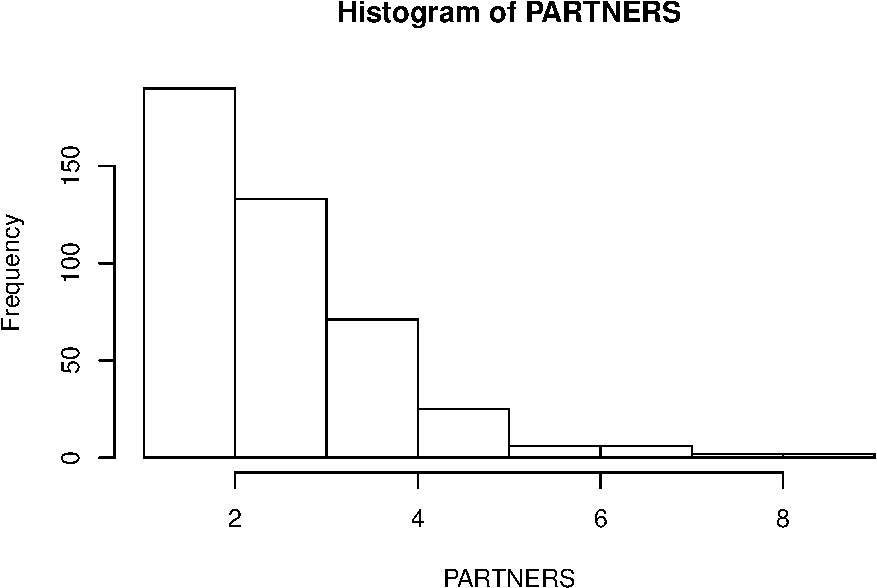
\includegraphics{prfe_files/figure-latex/unnamed-chunk-206-1.pdf}

The distribution of \texttt{PARTNERS} is severely non-normal. Instead of
attempting to transform the variable we will produce summary statistics
for each level of the \texttt{HIV} variable and perform a non-parametric
test:

\begin{Shaded}
\begin{Highlighting}[]
\KeywordTok{by}\NormalTok{(PARTNERS, HIV, summary)}
\KeywordTok{kruskal.test}\NormalTok{(PARTNERS }\OperatorTok{~}\StringTok{ }\NormalTok{HIV)}
\end{Highlighting}
\end{Shaded}

\begin{verbatim}
## HIV: 0
##    Min. 1st Qu.  Median    Mean 3rd Qu.    Max. 
##    1.00    2.00    3.00    2.72    3.00    8.00 
## -------------------------------------------------------- 
## HIV: 1
##    Min. 1st Qu.  Median    Mean 3rd Qu.    Max. 
##   1.000   4.000   5.000   5.381   7.000   9.000
\end{verbatim}

\begin{verbatim}
## 
##  Kruskal-Wallis rank sum test
## 
## data:  PARTNERS by HIV
## Kruskal-Wallis chi-squared = 32.036, df = 1, p-value = 1.514e-08
\end{verbatim}

An alternative way of looking at the data is as a tabulation:

\begin{Shaded}
\begin{Highlighting}[]
\KeywordTok{table}\NormalTok{(PARTNERS, HIV)}
\end{Highlighting}
\end{Shaded}

\begin{verbatim}
##         HIV
## PARTNERS   0   1
##        1  60   1
##        2 128   1
##        3 131   2
##        4  68   3
##        5  21   4
##        6   3   3
##        7   2   4
##        8   1   1
##        9   0   2
\end{verbatim}

You can use the \texttt{plot()} function to represent this table
graphically:

\begin{Shaded}
\begin{Highlighting}[]
\KeywordTok{plot}\NormalTok{(}\KeywordTok{table}\NormalTok{(PARTNERS, HIV), }\DataTypeTok{color =} \KeywordTok{c}\NormalTok{(}\StringTok{"lightgreen"}\NormalTok{, }\StringTok{"red"}\NormalTok{))}
\end{Highlighting}
\end{Shaded}

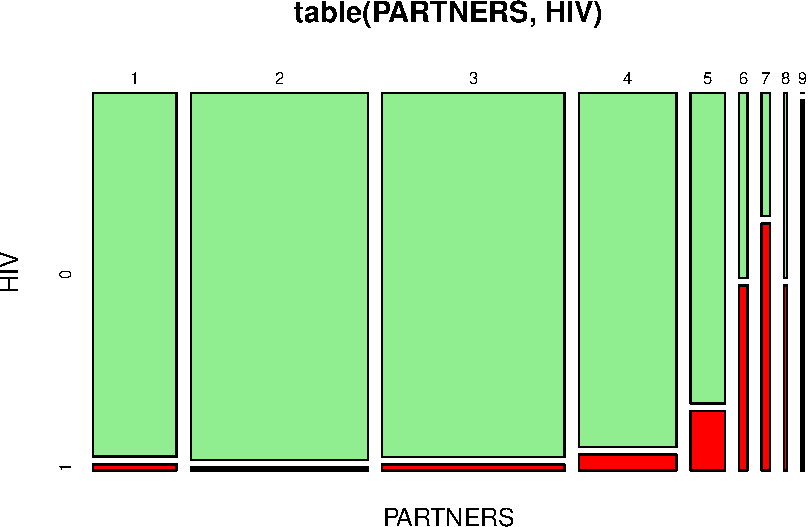
\includegraphics{prfe_files/figure-latex/unnamed-chunk-210-1.pdf}

There appears to be an association between the number of sexual
\texttt{PARTNERS} in the previous twelve months and positive
\texttt{HIV} serology. The proportion with positive \texttt{HIV}
serology increases as the number of sexual partners increases:

\begin{Shaded}
\begin{Highlighting}[]
\KeywordTok{prop.table}\NormalTok{(}\KeywordTok{table}\NormalTok{(PARTNERS, HIV), }\DecValTok{1}\NormalTok{) }\OperatorTok{*}\StringTok{ }\DecValTok{100}
\end{Highlighting}
\end{Shaded}

\begin{verbatim}
##         HIV
## PARTNERS           0           1
##        1  98.3606557   1.6393443
##        2  99.2248062   0.7751938
##        3  98.4962406   1.5037594
##        4  95.7746479   4.2253521
##        5  84.0000000  16.0000000
##        6  50.0000000  50.0000000
##        7  33.3333333  66.6666667
##        8  50.0000000  50.0000000
##        9   0.0000000 100.0000000
\end{verbatim}

The \textbf{`1'} instructs the \texttt{prop.table()} function to
calculate row proportions. You can also use the \texttt{plot()} function
to represent this table graphically:

\begin{Shaded}
\begin{Highlighting}[]
\KeywordTok{plot}\NormalTok{(}\KeywordTok{prop.table}\NormalTok{(}\KeywordTok{table}\NormalTok{(PARTNERS, HIV), }\DecValTok{1}\NormalTok{) }\OperatorTok{*}\StringTok{ }\DecValTok{100}\NormalTok{, }\DataTypeTok{color =} \KeywordTok{c}\NormalTok{(}\StringTok{"lightgreen"}\NormalTok{, }\StringTok{"red"}\NormalTok{))}
\end{Highlighting}
\end{Shaded}

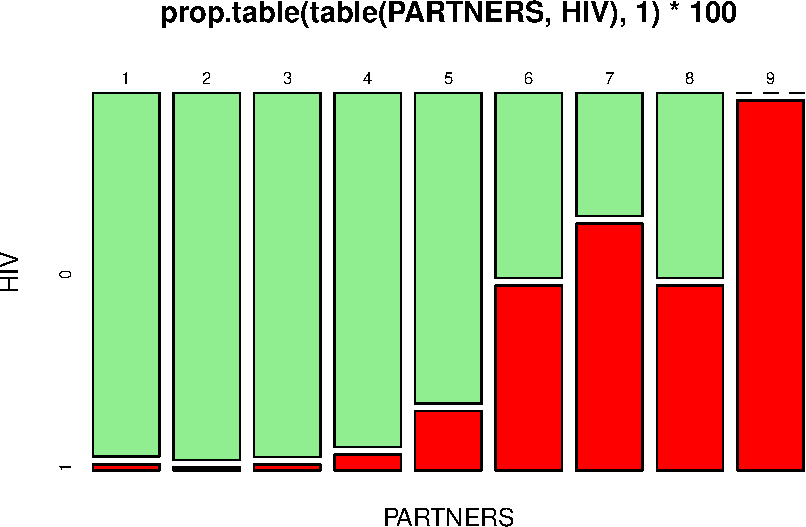
\includegraphics{prfe_files/figure-latex/unnamed-chunk-212-1.pdf}

The \emph{chi-square test for trend} is an appropriate test to perform
on this data. The \texttt{prop.trend.test()} function that performs the
\emph{chi-square test for trend} requires you to specify the
\emph{number of events} and the \emph{number of trials}. In this table:

\begin{Shaded}
\begin{Highlighting}[]
\KeywordTok{table}\NormalTok{(PARTNERS, HIV)}
\end{Highlighting}
\end{Shaded}

\begin{verbatim}
##         HIV
## PARTNERS   0   1
##        1  60   1
##        2 128   1
##        3 131   2
##        4  68   3
##        5  21   4
##        6   3   3
##        7   2   4
##        8   1   1
##        9   0   2
\end{verbatim}

The \emph{number of events} in each row is in the second column
(labelled \textbf{1}) and the \emph{number of trials} is the total
number of cases in each row of the table.

We can extract this data from a table object:

\begin{Shaded}
\begin{Highlighting}[]
\NormalTok{tab <-}\StringTok{ }\KeywordTok{table}\NormalTok{(PARTNERS, HIV)}
\NormalTok{events <-}\StringTok{ }\NormalTok{tab[ ,}\DecValTok{2}\NormalTok{]}
\NormalTok{trials <-}\StringTok{ }\NormalTok{tab[ ,}\DecValTok{1}\NormalTok{] }\OperatorTok{+}\StringTok{ }\NormalTok{tab[ ,}\DecValTok{2}\NormalTok{]}
\end{Highlighting}
\end{Shaded}

\begin{Shaded}
\begin{Highlighting}[]
\NormalTok{tab <-}\StringTok{ }\KeywordTok{table}\NormalTok{(PARTNERS, HIV)}
\NormalTok{events <-}\StringTok{ }\NormalTok{tab[ ,}\DecValTok{2}\NormalTok{]}
\NormalTok{trials <-}\StringTok{ }\NormalTok{tab[ ,}\DecValTok{1}\NormalTok{] }\OperatorTok{+}\StringTok{ }\NormalTok{tab[ ,}\DecValTok{2}\NormalTok{]}
\end{Highlighting}
\end{Shaded}

Another way of creating the \texttt{trials} object would be to use the
\texttt{apply()} function to sum the rows of the tab object:

\begin{Shaded}
\begin{Highlighting}[]
\NormalTok{trials <-}\StringTok{ }\KeywordTok{apply}\NormalTok{(tab, }\DecValTok{1}\NormalTok{, sum)}
\end{Highlighting}
\end{Shaded}

Pass this data to the \texttt{prop.trend.test()} function:

\begin{Shaded}
\begin{Highlighting}[]
\KeywordTok{prop.trend.test}\NormalTok{(events, trials)}
\end{Highlighting}
\end{Shaded}

\begin{verbatim}
## 
##  Chi-squared Test for Trend in Proportions
## 
## data:  events out of trials ,
##  using scores: 1 2 3 4 5 6 7 8 9
## X-squared = 76.389, df = 1, p-value < 2.2e-16
\end{verbatim}

With a linear trend such as this we can use \texttt{PARTNERS} in a
logistic model without recoding or creating indicator variables. We can
now specify and fit the logistic regression model:

\begin{Shaded}
\begin{Highlighting}[]
\NormalTok{gudhiv.lreg <-}\StringTok{ }\KeywordTok{glm}\NormalTok{(}\DataTypeTok{formula =}\NormalTok{ HIV }\OperatorTok{~}\StringTok{ }\NormalTok{GUD }\OperatorTok{+}\StringTok{ }\NormalTok{TRAVOUT }\OperatorTok{+}\StringTok{ }\NormalTok{PARTNERS,}
                   \DataTypeTok{family =} \KeywordTok{binomial}\NormalTok{(logit))}
\KeywordTok{summary}\NormalTok{(gudhiv.lreg)}
\end{Highlighting}
\end{Shaded}

\begin{verbatim}
## 
## Call:
## glm(formula = HIV ~ GUD + TRAVOUT + PARTNERS, family = binomial(logit))
## 
## Deviance Residuals: 
##      Min        1Q    Median        3Q       Max  
## -1.70415  -0.19849  -0.11148  -0.06247   3.11742  
## 
## Coefficients:
##             Estimate Std. Error z value Pr(>|z|)    
## (Intercept)  -9.4854     1.4663  -6.469 9.86e-11 ***
## GUD           1.3869     0.5937   2.336   0.0195 *  
## TRAVOUT       2.0867     0.9547   2.186   0.0288 *  
## PARTNERS      1.1605     0.2050   5.662 1.50e-08 ***
## ---
## Signif. codes:  0 '***' 0.001 '**' 0.01 '*' 0.05 '.' 0.1 ' ' 1
## 
## (Dispersion parameter for binomial family taken to be 1)
## 
##     Null deviance: 167.364  on 425  degrees of freedom
## Residual deviance:  99.377  on 422  degrees of freedom
##   (9 observations deleted due to missingness)
## AIC: 107.38
## 
## Number of Fisher Scoring iterations: 8
\end{verbatim}

We can use the \texttt{lreg.or()} function that we wrote earlier to
calculate and display odds ratios and confidence intervals:

\begin{Shaded}
\begin{Highlighting}[]
\KeywordTok{lreg.or}\NormalTok{(gudhiv.lreg)}
\end{Highlighting}
\end{Shaded}

\begin{verbatim}
##               OR  LCI   UCI
## (Intercept) 0.00 0.00  0.00
## GUD         4.00 1.25 12.81
## TRAVOUT     8.06 1.24 52.35
## PARTNERS    3.19 2.14  4.77
\end{verbatim}

\texttt{PARTNERS} is incorporated into the logistic model as a
continuous variable.

The odds ratio reported for \texttt{PARTNERS} is the odds ratio
associated with a unit increase in the number of sexual
\texttt{PARTNERS}. A man reporting five sexual partners, for example,
was over three times as likely (odds ratio = 3.19) to have a positive
HIV-2 serology than a man reporting four sexual partners.

An alternative approach would be to have created an \emph{indicator}
variables:

\begin{Shaded}
\begin{Highlighting}[]
\NormalTok{part.gt}\FloatTok{.5}\NormalTok{ <-}\StringTok{ }\KeywordTok{ifelse}\NormalTok{(PARTNERS }\OperatorTok{>}\StringTok{ }\DecValTok{5}\NormalTok{, }\DecValTok{1}\NormalTok{, }\DecValTok{0}\NormalTok{)}
\end{Highlighting}
\end{Shaded}

This creates a new variable (\texttt{part.gt.5}) that indicates whether
or not an individual subject reported having more than five sexual
partners in the previous twelve months:

\begin{Shaded}
\begin{Highlighting}[]
\KeywordTok{table}\NormalTok{(PARTNERS, part.gt}\FloatTok{.5}\NormalTok{)}
\end{Highlighting}
\end{Shaded}

\begin{verbatim}
##         part.gt.5
## PARTNERS   0   1
##        1  61   0
##        2 129   0
##        3 133   0
##        4  71   0
##        5  25   0
##        6   0   6
##        7   0   6
##        8   0   2
##        9   0   2
\end{verbatim}

You can also inspect this on a case-by-case basis:

\begin{Shaded}
\begin{Highlighting}[]
\KeywordTok{cbind}\NormalTok{(PARTNERS, part.gt}\FloatTok{.5}\NormalTok{)}
\end{Highlighting}
\end{Shaded}

\begin{verbatim}
##        PARTNERS part.gt.5
##   [1,]        2         0
##   [2,]        2         0
##   [3,]        1         0
##   [4,]        2         0
##   [5,]        3         0
##   [6,]        2         0
##   [7,]        4         0
##   [8,]        5         0
##   [9,]        2         0
##  [10,]        3         0
##  [11,]        4         0
##  [12,]        3         0
##  [13,]        1         0
##  [14,]        2         0
##  [15,]        5         0
##  [16,]        8         1
##  [17,]        5         0
##  [18,]        3         0
##  [19,]        2         0
##  [20,]        1         0
##  [21,]        2         0
##  [22,]        3         0
##  [23,]        2         0
##  [24,]        3         0
##  [25,]        4         0
##  [26,]        3         0
##  [27,]        4         0
##  [28,]        3         0
##  [29,]        4         0
##  [30,]        5         0
##  [31,]        4         0
##  [32,]        3         0
##  [33,]        4         0
##  [34,]        5         0
##  [35,]        2         0
##  [36,]        4         0
##  [37,]        3         0
##  [38,]        2         0
##  [39,]        1         0
##  [40,]        2         0
##  [41,]        3         0
##  [42,]        4         0
##  [43,]        3         0
##  [44,]        3         0
##  [45,]        2         0
##  [46,]        4         0
##  [47,]        5         0
##  [48,]        4         0
##  [49,]        3         0
##  [50,]        4         0
##  [51,]        1         0
##  [52,]        1         0
##  [53,]        2         0
##  [54,]        3         0
##  [55,]        3         0
##  [56,]        3         0
##  [57,]        3         0
##  [58,]        4         0
##  [59,]        5         0
##  [60,]        4         0
##  [61,]        3         0
##  [62,]        3         0
##  [63,]        5         0
##  [64,]        2         0
##  [65,]        2         0
##  [66,]        3         0
##  [67,]        2         0
##  [68,]        1         0
##  [69,]        2         0
##  [70,]        3         0
##  [71,]        2         0
##  [72,]        3         0
##  [73,]        4         0
##  [74,]        3         0
##  [75,]        3         0
##  [76,]        2         0
##  [77,]        5         0
##  [78,]        4         0
##  [79,]        3         0
##  [80,]        1         0
##  [81,]        2         0
##  [82,]        5         0
##  [83,]        3         0
##  [84,]        7         1
##  [85,]        6         1
##  [86,]        5         0
##  [87,]        5         0
##  [88,]        5         0
##  [89,]        4         0
##  [90,]        3         0
##  [91,]        2         0
##  [92,]        5         0
##  [93,]        1         0
##  [94,]        1         0
##  [95,]        1         0
##  [96,]        1         0
##  [97,]        2         0
##  [98,]        3         0
##  [99,]        4         0
## [100,]        3         0
## [101,]        3         0
## [102,]        2         0
## [103,]        3         0
## [104,]        4         0
## [105,]        3         0
## [106,]        2         0
## [107,]        3         0
## [108,]        4         0
## [109,]        3         0
## [110,]        3         0
## [111,]        4         0
## [112,]        3         0
## [113,]        6         1
## [114,]        3         0
## [115,]        4         0
## [116,]        3         0
## [117,]        3         0
## [118,]        2         0
## [119,]        3         0
## [120,]        4         0
## [121,]        7         1
## [122,]        3         0
## [123,]        2         0
## [124,]        3         0
## [125,]        4         0
## [126,]        3         0
## [127,]        2         0
## [128,]        3         0
## [129,]        4         0
## [130,]        8         1
## [131,]        5         0
## [132,]        6         1
## [133,]        5         0
## [134,]        4         0
## [135,]        4         0
## [136,]        4         0
## [137,]        3         0
## [138,]        4         0
## [139,]        3         0
## [140,]        3         0
## [141,]        2         0
## [142,]        2         0
## [143,]        1         0
## [144,]        2         0
## [145,]        1         0
## [146,]        2         0
## [147,]        3         0
## [148,]        1         0
## [149,]        2         0
## [150,]        3         0
## [151,]        2         0
## [152,]        2         0
## [153,]        2         0
## [154,]        1         0
## [155,]        1         0
## [156,]        2         0
## [157,]        3         0
## [158,]        3         0
## [159,]        2         0
## [160,]        3         0
## [161,]        4         0
## [162,]        2         0
## [163,]        5         0
## [164,]        4         0
## [165,]        2         0
## [166,]        3         0
## [167,]        2         0
## [168,]        2         0
## [169,]        1         0
## [170,]        4         0
## [171,]        3         0
## [172,]        3         0
## [173,]        2         0
## [174,]        3         0
## [175,]        2         0
## [176,]        4         0
## [177,]        3         0
## [178,]        2         0
## [179,]        3         0
## [180,]        4         0
## [181,]        2         0
## [182,]        3         0
## [183,]        3         0
## [184,]        4         0
## [185,]        2         0
## [186,]        3         0
## [187,]        2         0
## [188,]        2         0
## [189,]        3         0
## [190,]        3         0
## [191,]        2         0
## [192,]        3         0
## [193,]        2         0
## [194,]        4         0
## [195,]        3         0
## [196,]        2         0
## [197,]        2         0
## [198,]        3         0
## [199,]        2         0
## [200,]        3         0
## [201,]        2         0
## [202,]        3         0
## [203,]        3         0
## [204,]        2         0
## [205,]        3         0
## [206,]        2         0
## [207,]        3         0
## [208,]        2         0
## [209,]        1         0
## [210,]        6         1
## [211,]        9         1
## [212,]        1         0
## [213,]        2         0
## [214,]        3         0
## [215,]        4         0
## [216,]        5         0
## [217,]        4         0
## [218,]        5         0
## [219,]        5         0
## [220,]        5         0
## [221,]        4         0
## [222,]        3         0
## [223,]        4         0
## [224,]        3         0
## [225,]        2         0
## [226,]        1         0
## [227,]        2         0
## [228,]        3         0
## [229,]        2         0
## [230,]        1         0
## [231,]        4         0
## [232,]        3         0
## [233,]        4         0
## [234,]        3         0
## [235,]        3         0
## [236,]        2         0
## [237,]        2         0
## [238,]        1         0
## [239,]        2         0
## [240,]        3         0
## [241,]        2         0
## [242,]        1         0
## [243,]        2         0
## [244,]        4         0
## [245,]        3         0
## [246,]        2         0
## [247,]        3         0
## [248,]        2         0
## [249,]        2         0
## [250,]        1         0
## [251,]        2         0
## [252,]        3         0
## [253,]        2         0
## [254,]        3         0
## [255,]        1         0
## [256,]        2         0
## [257,]        3         0
## [258,]        2         0
## [259,]        4         0
## [260,]        3         0
## [261,]        3         0
## [262,]        2         0
## [263,]        2         0
## [264,]        1         0
## [265,]        1         0
## [266,]        1         0
## [267,]        1         0
## [268,]        1         0
## [269,]        1         0
## [270,]        1         0
## [271,]        1         0
## [272,]        1         0
## [273,]        1         0
## [274,]        2         0
## [275,]        3         0
## [276,]        2         0
## [277,]        3         0
## [278,]        2         0
## [279,]        1         0
## [280,]        2         0
## [281,]        3         0
## [282,]        4         0
## [283,]        3         0
## [284,]        2         0
## [285,]        3         0
## [286,]        2         0
## [287,]        1         0
## [288,]        2         0
## [289,]        4         0
## [290,]        7         1
## [291,]        1         0
## [292,]        4         0
## [293,]        1         0
## [294,]        3         0
## [295,]        3         0
## [296,]        4         0
## [297,]        3         0
## [298,]        2         0
## [299,]        2         0
## [300,]        1         0
## [301,]        2         0
## [302,]        3         0
## [303,]        3         0
## [304,]        3         0
## [305,]        2         0
## [306,]        4         0
## [307,]        4         0
## [308,]        5         0
## [309,]        4         0
## [310,]        4         0
## [311,]        9         1
## [312,]        3         0
## [313,]        3         0
## [314,]        2         0
## [315,]        2         0
## [316,]        1         0
## [317,]        1         0
## [318,]        2         0
## [319,]        7         1
## [320,]        3         0
## [321,]        2         0
## [322,]        1         0
## [323,]        2         0
## [324,]        4         0
## [325,]        6         1
## [326,]        5         0
## [327,]        3         0
## [328,]        2         0
## [329,]        3         0
## [330,]        4         0
## [331,]        3         0
## [332,]        2         0
## [333,]        3         0
## [334,]        4         0
## [335,]        3         0
## [336,]        3         0
## [337,]        2         0
## [338,]        3         0
## [339,]        4         0
## [340,]        3         0
## [341,]        2         0
## [342,]        3         0
## [343,]        1         0
## [344,]        1         0
## [345,]        2         0
## [346,]        3         0
## [347,]        4         0
## [348,]        3         0
## [349,]        3         0
## [350,]        2         0
## [351,]        4         0
## [352,]        5         0
## [353,]        4         0
## [354,]        3         0
## [355,]        3         0
## [356,]        2         0
## [357,]        2         0
## [358,]        1         0
## [359,]        4         0
## [360,]        1         0
## [361,]        1         0
## [362,]        4         0
## [363,]        3         0
## [364,]        2         0
## [365,]        1         0
## [366,]        4         0
## [367,]        1         0
## [368,]        2         0
## [369,]        3         0
## [370,]        1         0
## [371,]        5         0
## [372,]        4         0
## [373,]        3         0
## [374,]        2         0
## [375,]        1         0
## [376,]        2         0
## [377,]        3         0
## [378,]        2         0
## [379,]        4         0
## [380,]        2         0
## [381,]        3         0
## [382,]        4         0
## [383,]        7         1
## [384,]        3         0
## [385,]        2         0
## [386,]        4         0
## [387,]        4         0
## [388,]        3         0
## [389,]        2         0
## [390,]        2         0
## [391,]        1         0
## [392,]        2         0
## [393,]        6         1
## [394,]        7         1
## [395,]        2         0
## [396,]        1         0
## [397,]        2         0
## [398,]        3         0
## [399,]        1         0
## [400,]        2         0
## [401,]        3         0
## [402,]        2         0
## [403,]        1         0
## [404,]        2         0
## [405,]        3         0
## [406,]        2         0
## [407,]        3         0
## [408,]        2         0
## [409,]        3         0
## [410,]        2         0
## [411,]        4         0
## [412,]        2         0
## [413,]        2         0
## [414,]        1         0
## [415,]        2         0
## [416,]        3         0
## [417,]        2         0
## [418,]        3         0
## [419,]        2         0
## [420,]        3         0
## [421,]        2         0
## [422,]        3         0
## [423,]        4         0
## [424,]        2         0
## [425,]        2         0
## [426,]        3         0
## [427,]        4         0
## [428,]        4         0
## [429,]        1         0
## [430,]        2         0
## [431,]        3         0
## [432,]        2         0
## [433,]        1         0
## [434,]        1         0
## [435,]        2         0
\end{verbatim}

We can now specify and fit the logistic regression model using our
indicator variable:

\begin{Shaded}
\begin{Highlighting}[]
\NormalTok{gudhiv.lreg <-}\StringTok{ }\KeywordTok{glm}\NormalTok{(}\DataTypeTok{formula =}\NormalTok{ HIV }\OperatorTok{~}\StringTok{ }\NormalTok{GUD }\OperatorTok{+}\StringTok{ }\NormalTok{TRAVOUT }\OperatorTok{+}\StringTok{ }\NormalTok{part.gt}\FloatTok{.5}\NormalTok{,}
                   \DataTypeTok{family =} \KeywordTok{binomial}\NormalTok{(logit))}
\KeywordTok{summary}\NormalTok{(gudhiv.lreg)}
\KeywordTok{lreg.or}\NormalTok{(gudhiv.lreg)}
\end{Highlighting}
\end{Shaded}

\begin{verbatim}
## 
## Call:
## glm(formula = HIV ~ GUD + TRAVOUT + part.gt.5, family = binomial(logit))
## 
## Deviance Residuals: 
##     Min       1Q   Median       3Q      Max  
## -1.6092  -0.2205  -0.2205  -0.0719   3.4521  
## 
## Coefficients:
##             Estimate Std. Error z value Pr(>|z|)    
## (Intercept)  -5.9559     0.9850  -6.046 1.48e-09 ***
## GUD           1.4930     0.5805   2.572   0.0101 *  
## TRAVOUT       2.2514     0.9319   2.416   0.0157 *  
## part.gt.5     4.6791     0.7560   6.189 6.05e-10 ***
## ---
## Signif. codes:  0 '***' 0.001 '**' 0.01 '*' 0.05 '.' 0.1 ' ' 1
## 
## (Dispersion parameter for binomial family taken to be 1)
## 
##     Null deviance: 167.36  on 425  degrees of freedom
## Residual deviance: 106.43  on 422  degrees of freedom
##   (9 observations deleted due to missingness)
## AIC: 114.43
## 
## Number of Fisher Scoring iterations: 7
\end{verbatim}

\begin{verbatim}
##                 OR   LCI    UCI
## (Intercept)   0.00  0.00   0.02
## GUD           4.45  1.43  13.89
## TRAVOUT       9.50  1.53  59.02
## part.gt.5   107.67 24.47 473.84
\end{verbatim}

We can now quit R:

\begin{Shaded}
\begin{Highlighting}[]
\KeywordTok{q}\NormalTok{()}
\end{Highlighting}
\end{Shaded}

For this exercise there is no need to save the workspace image so click
the \textbf{No} or \textbf{Don't Save} button (GUI) or enter \texttt{n}
when prompted to save the workspace image (terminal).

\hypertarget{summary-3}{%
\section{Summary}\label{summary-3}}

\begin{itemize}
\item
  Using built-in functions and our own functions we can use \texttt{R}
  to analyse epidemiological data.
\item
  The power of \texttt{R} is that it can be easily extended. Many
  user-contributed functions (usually packages of related functions) are
  available for download over the Internet. We will use one of these
  packages in the next exercise.
\end{itemize}

\hypertarget{exercise5}{%
\chapter{Extending R with packages}\label{exercise5}}

\texttt{R} has no built-in functions for survival analysis but, because
it is an extensible system, survival analysis is available as an add-in
package. You can find a list of add-in packages at the \texttt{R}
website.

\url{http://www.r-project.org/}

Add-in packages are installed from the Internet. There are a series of
\texttt{R} functions that enable you to download and install add-in
packages.

The \texttt{survival} package adds functions to \texttt{R} that enable
it to analyse survival data. This package may be downloaded and
installed using \texttt{install.packages("survival")} or from the
\texttt{Packages} or \texttt{Packages\ \&\ Data} menu if you are using a
GUI version of \texttt{R}.

Packages are loaded into \texttt{R} as they are needed using the
\texttt{library()} function. Start \texttt{R} and load the
\texttt{survival} package:

\begin{Shaded}
\begin{Highlighting}[]
\KeywordTok{library}\NormalTok{(survival)}
\end{Highlighting}
\end{Shaded}

Before we go any further we should retrieve a dataset:

\begin{Shaded}
\begin{Highlighting}[]
\NormalTok{ca <-}\StringTok{ }\KeywordTok{read.table}\NormalTok{(}\StringTok{"ca.dat"}\NormalTok{, }\DataTypeTok{header =} \OtherTok{TRUE}\NormalTok{)}
\KeywordTok{attach}\NormalTok{(ca)}
\end{Highlighting}
\end{Shaded}

\begin{verbatim}
## The following objects are masked from ca (pos = 8):
## 
##     group, status, time
\end{verbatim}

The columns in this dataset on the survival of cancer patients in two
different treatment groups are as follows:

\begin{longtable}[]{@{}ll@{}}
\toprule
\begin{minipage}[t]{0.21\columnwidth}\raggedright
\textbf{time}\strut
\end{minipage} & \begin{minipage}[t]{0.54\columnwidth}\raggedright
Survival or censoring time (months)\strut
\end{minipage}\tabularnewline
\begin{minipage}[t]{0.21\columnwidth}\raggedright
\textbf{status}\strut
\end{minipage} & \begin{minipage}[t]{0.54\columnwidth}\raggedright
Censoring status (1=dead, 0=censored)\strut
\end{minipage}\tabularnewline
\begin{minipage}[t]{0.21\columnwidth}\raggedright
\textbf{group}\strut
\end{minipage} & \begin{minipage}[t]{0.54\columnwidth}\raggedright
Treatment group (1 / 2)\strut
\end{minipage}\tabularnewline
\bottomrule
\end{longtable}

We next need to create a \texttt{survival} object from the \texttt{time}
and \texttt{status} variables using the \texttt{Surv()} function:

\begin{Shaded}
\begin{Highlighting}[]
\NormalTok{response <-}\StringTok{ }\KeywordTok{Surv}\NormalTok{(time, status)}
\end{Highlighting}
\end{Shaded}

We can then specify the model for the survival analysis. In this case we
state that survival (\texttt{response}) is dependent upon the treatment
\texttt{group}:

\begin{Shaded}
\begin{Highlighting}[]
\NormalTok{ca.surv <-}\StringTok{ }\KeywordTok{survfit}\NormalTok{(response }\OperatorTok{~}\StringTok{ }\NormalTok{group)}
\end{Highlighting}
\end{Shaded}

The \texttt{summary()} function applied to a \texttt{survfit} object
lists the survival probabilities at each time point with 95\% confidence
intervals:

\begin{Shaded}
\begin{Highlighting}[]
\KeywordTok{summary}\NormalTok{(ca.surv)}
\end{Highlighting}
\end{Shaded}

\begin{verbatim}
## Call: survfit(formula = response ~ group)
## 
##                 group=1 
##  time n.risk n.event survival std.err lower 95% CI upper 95% CI
##     8     22       1    0.955  0.0444       0.8714        1.000
##     9     21       1    0.909  0.0613       0.7966        1.000
##    13     19       1    0.861  0.0744       0.7270        1.000
##    14     17       1    0.811  0.0856       0.6591        0.997
##    18     16       1    0.760  0.0940       0.5963        0.968
##    19     15       1    0.709  0.1005       0.5373        0.936
##    21     14       1    0.659  0.1053       0.4814        0.901
##    23     13       1    0.608  0.1087       0.4282        0.863
##    30     10       1    0.547  0.1136       0.3643        0.822
##    31      9       1    0.486  0.1161       0.3046        0.776
##    32      8       1    0.426  0.1164       0.2489        0.727
##    34      7       1    0.365  0.1146       0.1971        0.675
##    48      5       1    0.292  0.1125       0.1371        0.621
##    56      3       1    0.195  0.1092       0.0647        0.585
## 
##                 group=2 
##  time n.risk n.event survival std.err lower 95% CI upper 95% CI
##     4     24       1   0.9583  0.0408      0.88163        1.000
##     5     23       2   0.8750  0.0675      0.75221        1.000
##     6     21       1   0.8333  0.0761      0.69681        0.997
##     7     20       1   0.7917  0.0829      0.64478        0.972
##     8     19       2   0.7083  0.0928      0.54795        0.916
##     9     17       1   0.6667  0.0962      0.50240        0.885
##    11     16       1   0.6250  0.0988      0.45845        0.852
##    12     15       1   0.5833  0.1006      0.41598        0.818
##    21     12       1   0.5347  0.1033      0.36614        0.781
##    23     11       1   0.4861  0.1047      0.31866        0.742
##    27     10       1   0.4375  0.1049      0.27340        0.700
##    28      9       1   0.3889  0.1039      0.23032        0.657
##    30      8       1   0.3403  0.1017      0.18945        0.611
##    32      7       1   0.2917  0.0981      0.15088        0.564
##    33      6       1   0.2431  0.0930      0.11481        0.515
##    37      5       1   0.1944  0.0862      0.08157        0.464
##    41      4       2   0.0972  0.0650      0.02624        0.360
##    43      2       1   0.0486  0.0473      0.00722        0.327
##    45      1       1   0.0000     NaN           NA           NA
\end{verbatim}

Printing the \texttt{ca.surv} object provides another view of the
results:

\begin{Shaded}
\begin{Highlighting}[]
\NormalTok{ca.surv}
\end{Highlighting}
\end{Shaded}

\begin{verbatim}
## Call: survfit(formula = response ~ group)
## 
##          n events median 0.95LCL 0.95UCL
## group=1 22     14     31      21      NA
## group=2 24     22     23      11      37
\end{verbatim}

The \texttt{plot()} function with a \texttt{survfit} object displays the
survival curves:

\begin{Shaded}
\begin{Highlighting}[]
\KeywordTok{plot}\NormalTok{(ca.surv, }\DataTypeTok{xlab =} \StringTok{"Months"}\NormalTok{, }\DataTypeTok{ylab =} \StringTok{"Survival"}\NormalTok{)}
\end{Highlighting}
\end{Shaded}

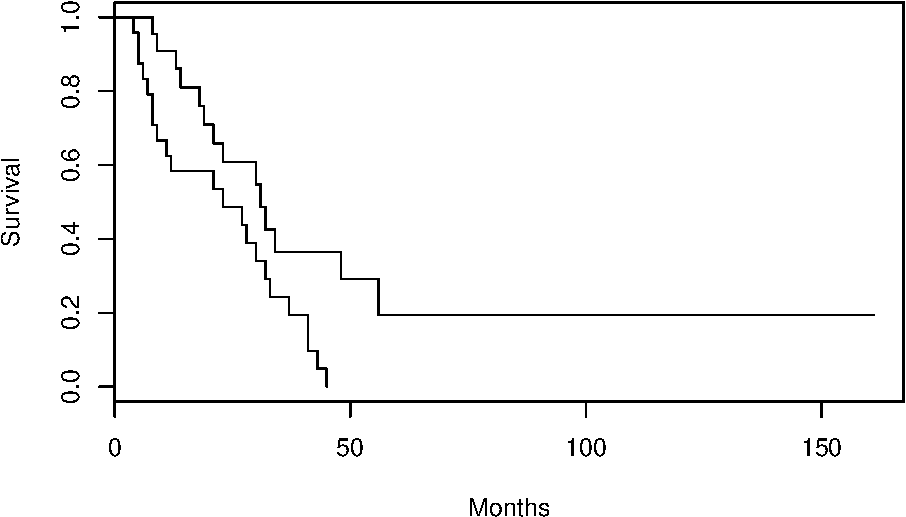
\includegraphics{prfe_files/figure-latex/unnamed-chunk-232-1.pdf}

We can make it easier to distinguish between the two lines by specifying
a width for each line using thelwd parameter of the \texttt{plot()}
function:

\begin{Shaded}
\begin{Highlighting}[]
\KeywordTok{plot}\NormalTok{(ca.surv, }\DataTypeTok{xlab =} \StringTok{"Months"}\NormalTok{, }\DataTypeTok{ylab =} \StringTok{"Survival"}\NormalTok{, }\DataTypeTok{lwd =} \KeywordTok{c}\NormalTok{(}\DecValTok{1}\NormalTok{, }\DecValTok{2}\NormalTok{))}
\end{Highlighting}
\end{Shaded}

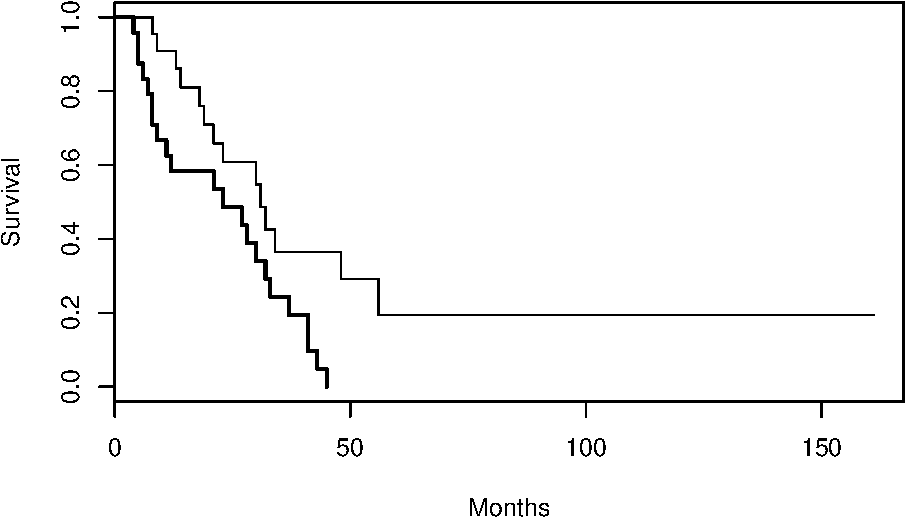
\includegraphics{prfe_files/figure-latex/unnamed-chunk-233-1.pdf}

It would also be useful to add a legend:

\begin{Shaded}
\begin{Highlighting}[]
\KeywordTok{legend}\NormalTok{(}\DecValTok{125}\NormalTok{, }\DecValTok{1}\NormalTok{, }\KeywordTok{names}\NormalTok{(ca.surv}\OperatorTok{$}\NormalTok{strata), }\DataTypeTok{lwd =} \KeywordTok{c}\NormalTok{(}\DecValTok{1}\NormalTok{, }\DecValTok{2}\NormalTok{))}
\end{Highlighting}
\end{Shaded}

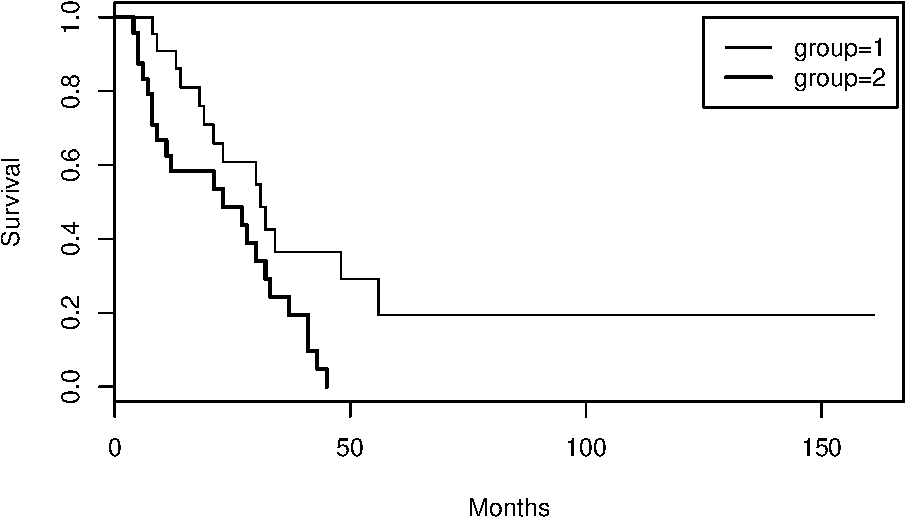
\includegraphics{prfe_files/figure-latex/unnamed-chunk-235-1.pdf}

If there is only one survival curve to plot then plotting a
\texttt{survfit} object will plot the survival curve with 95\%
confidence limits. You can specify that confidence limits should be
plotted when there is more than one survival curve but the results can
be disappointing:

\begin{Shaded}
\begin{Highlighting}[]
\KeywordTok{plot}\NormalTok{(ca.surv, }\DataTypeTok{conf.int =} \OtherTok{TRUE}\NormalTok{)}
\end{Highlighting}
\end{Shaded}

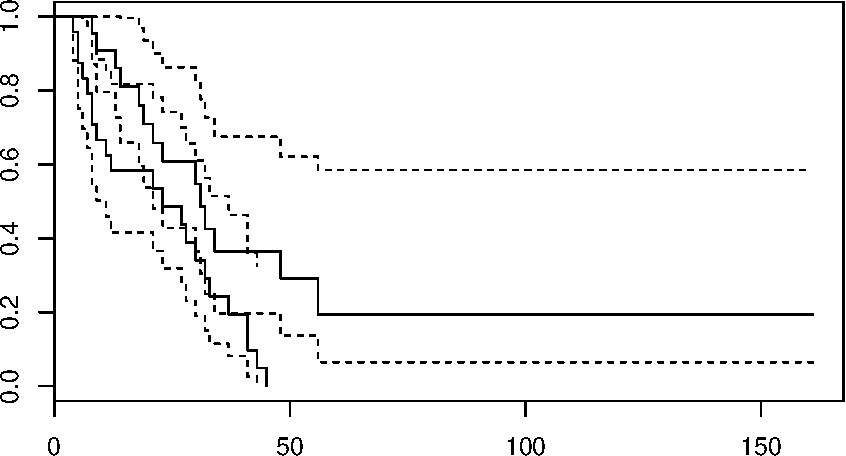
\includegraphics{prfe_files/figure-latex/unnamed-chunk-236-1.pdf}

Plots can be improved by specifying different colours for each curve:

\begin{Shaded}
\begin{Highlighting}[]
\KeywordTok{plot}\NormalTok{(ca.surv, }\DataTypeTok{conf.int =} \OtherTok{TRUE}\NormalTok{, }\DataTypeTok{col =} \KeywordTok{c}\NormalTok{(}\StringTok{"red"}\NormalTok{, }\StringTok{"darkgreen"}\NormalTok{))}
\end{Highlighting}
\end{Shaded}

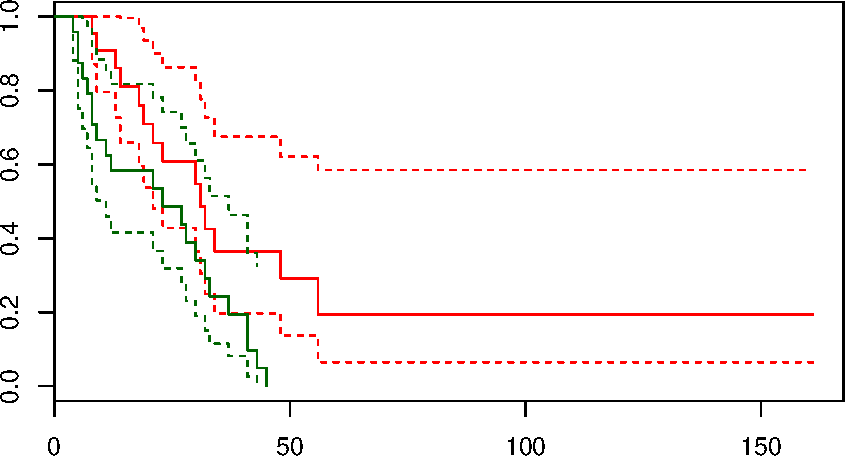
\includegraphics{prfe_files/figure-latex/unnamed-chunk-237-1.pdf}

We can perform a formal test of the two survival times using the
\texttt{survdiff()} function:

\begin{Shaded}
\begin{Highlighting}[]
\KeywordTok{survdiff}\NormalTok{(response }\OperatorTok{~}\StringTok{ }\NormalTok{group)}
\end{Highlighting}
\end{Shaded}

\begin{verbatim}
## Call:
## survdiff(formula = response ~ group)
## 
##          N Observed Expected (O-E)^2/E (O-E)^2/V
## group=1 22       14     21.1      2.38      6.26
## group=2 24       22     14.9      3.36      6.26
## 
##  Chisq= 6.3  on 1 degrees of freedom, p= 0.0123
\end{verbatim}

We can now quit \texttt{R}:

\begin{Shaded}
\begin{Highlighting}[]
\KeywordTok{q}\NormalTok{()}
\end{Highlighting}
\end{Shaded}

For this exercise there is no need to save the workspace image so click
the \textbf{No} or \textbf{Don't Save} button (GUI) or enter \texttt{n}
when prompted to save the workspace image (terminal).

\hypertarget{summary-4}{%
\section{Summary}\label{summary-4}}

\begin{itemize}
\item
  \texttt{R} can be extended by adding additional packages. Some
  packages are included with the standard \texttt{R} installation but
  many others are available and may be downloaded from the Internet.
\item
  You can find a list of add-in packages at the \texttt{R} website:
  \url{http://www.r-project.org/}
\item
  Packages may also be downloaded and installed from this site using the
  \texttt{install.packages()} function or from the \textbf{Packages} or
  \textbf{Packages \& Data} menu if you are using a GUI version of
  \texttt{R}.
\item
  Packages are loaded into \texttt{R} as they are needed using the
  \texttt{library()} function. You can use the \texttt{search()}
  function to display a list of loaded packages and attached
  data.frames.
\end{itemize}

\hypertarget{exercise6}{%
\chapter{Making your own objects behave like R
objects}\label{exercise6}}

In the previous exercises we concentrated on writing functions that take
some input data, analyse it, and display the results of the analysis.
The standard \texttt{R} functions we have used all do this. The
\texttt{fisher.test()} function, for example, takes a \texttt{table}
object (or the names of two variables) as input and calculates and
displays the p- value for \emph{Fisher's exact test} and the odds ratio
and associated confidence interval for two-by-two tables:

\begin{Shaded}
\begin{Highlighting}[]
\NormalTok{fem <-}\StringTok{ }\KeywordTok{read.table}\NormalTok{(}\StringTok{"fem.dat"}\NormalTok{, }\DataTypeTok{header =} \OtherTok{TRUE}\NormalTok{)}
\KeywordTok{attach}\NormalTok{(fem)}
\end{Highlighting}
\end{Shaded}

\begin{verbatim}
## The following objects are masked from fem (pos = 6):
## 
##     AGE, ANX, DEP, ID, IQ, LIFE, SEX, SLP, WT
\end{verbatim}

\begin{verbatim}
## The following objects are masked from fem (pos = 7):
## 
##     AGE, ANX, DEP, ID, IQ, LIFE, SEX, SLP, WT
\end{verbatim}

\begin{verbatim}
## The following objects are masked from fem (pos = 8):
## 
##     AGE, ANX, DEP, ID, IQ, LIFE, SEX, SLP, WT
\end{verbatim}

\begin{verbatim}
## The following objects are masked from fem (pos = 13):
## 
##     AGE, ANX, DEP, ID, IQ, LIFE, SEX, SLP, WT
\end{verbatim}

\begin{Shaded}
\begin{Highlighting}[]
\KeywordTok{fisher.test}\NormalTok{(SEX, LIFE)}
\end{Highlighting}
\end{Shaded}

\begin{verbatim}
## 
##  Fisher's Exact Test for Count Data
## 
## data:  SEX and LIFE
## p-value = 0.03175
## alternative hypothesis: true odds ratio is not equal to 1
## 95 percent confidence interval:
##   1.080298 14.214482
## sample estimates:
## odds ratio 
##   3.620646
\end{verbatim}

The results of the \texttt{fisher.test()} function may also be saved for
later use:

\begin{Shaded}
\begin{Highlighting}[]
\NormalTok{ft <-}\StringTok{ }\KeywordTok{fisher.test}\NormalTok{(SEX, LIFE)}
\NormalTok{ft}
\end{Highlighting}
\end{Shaded}

\begin{verbatim}
## 
##  Fisher's Exact Test for Count Data
## 
## data:  SEX and LIFE
## p-value = 0.03175
## alternative hypothesis: true odds ratio is not equal to 1
## 95 percent confidence interval:
##   1.080298 14.214482
## sample estimates:
## odds ratio 
##   3.620646
\end{verbatim}

The \texttt{fisher.test()} function returns an object of the class
\texttt{htest}:

\begin{Shaded}
\begin{Highlighting}[]
\KeywordTok{class}\NormalTok{(ft)}
\end{Highlighting}
\end{Shaded}

\begin{verbatim}
## [1] "htest"
\end{verbatim}

which is a list containing the output of the \texttt{fisher.test()}
function. Each item of output is stored as a different named item in the
list:

\begin{Shaded}
\begin{Highlighting}[]
\KeywordTok{names}\NormalTok{(ft)}
\KeywordTok{str}\NormalTok{(ft)}
\end{Highlighting}
\end{Shaded}

\begin{verbatim}
## [1] "p.value"     "conf.int"    "estimate"    "null.value"  "alternative"
## [6] "method"      "data.name"
\end{verbatim}

\begin{verbatim}
## List of 7
##  $ p.value    : num 0.0318
##  $ conf.int   : atomic [1:2] 1.08 14.21
##   ..- attr(*, "conf.level")= num 0.95
##  $ estimate   : Named num 3.62
##   ..- attr(*, "names")= chr "odds ratio"
##  $ null.value : Named num 1
##   ..- attr(*, "names")= chr "odds ratio"
##  $ alternative: chr "two.sided"
##  $ method     : chr "Fisher's Exact Test for Count Data"
##  $ data.name  : chr "SEX and LIFE"
##  - attr(*, "class")= chr "htest"
\end{verbatim}

Each of these items can be referred to by name:

\begin{Shaded}
\begin{Highlighting}[]
\NormalTok{ft}\OperatorTok{$}\NormalTok{estimate}
\NormalTok{ft}\OperatorTok{$}\NormalTok{conf.int}
\end{Highlighting}
\end{Shaded}

\begin{verbatim}
## odds ratio 
##   3.620646
\end{verbatim}

\begin{verbatim}
## [1]  1.080298 14.214482
## attr(,"conf.level")
## [1] 0.95
\end{verbatim}

When you display the output of the \texttt{fisher.test()} function
either by calling the function directly:

\begin{Shaded}
\begin{Highlighting}[]
\KeywordTok{fisher.test}\NormalTok{(SEX, LIFE)}
\end{Highlighting}
\end{Shaded}

\begin{verbatim}
## 
##  Fisher's Exact Test for Count Data
## 
## data:  SEX and LIFE
## p-value = 0.03175
## alternative hypothesis: true odds ratio is not equal to 1
## 95 percent confidence interval:
##   1.080298 14.214482
## sample estimates:
## odds ratio 
##   3.620646
\end{verbatim}

or by typing the name of an object created using the
\texttt{fisher.test()} function:

\begin{Shaded}
\begin{Highlighting}[]
\NormalTok{ft}
\end{Highlighting}
\end{Shaded}

\begin{verbatim}
## 
##  Fisher's Exact Test for Count Data
## 
## data:  SEX and LIFE
## p-value = 0.03175
## alternative hypothesis: true odds ratio is not equal to 1
## 95 percent confidence interval:
##   1.080298 14.214482
## sample estimates:
## odds ratio 
##   3.620646
\end{verbatim}

The \texttt{print()} function takes over and formatted output is
produced. The \texttt{print()} function knows about \texttt{htest} class
objects and produces output of the correct format for that class of
object. This means that any function that produces an \texttt{htest}
object (or any other standard \texttt{R} object) does not need to
include \texttt{R} commands to produce formatted output.

All hypothesis testing functions supplied with \texttt{R} produce
objects of the htest class and use the \texttt{print()} function to
produce formatted output. For example:

\begin{Shaded}
\begin{Highlighting}[]
\NormalTok{tt <-}\StringTok{ }\KeywordTok{t.test}\NormalTok{(WT }\OperatorTok{~}\StringTok{ }\NormalTok{LIFE)}
\KeywordTok{class}\NormalTok{(tt)}
\NormalTok{tt}
\end{Highlighting}
\end{Shaded}

\begin{verbatim}
## [1] "htest"
\end{verbatim}

\begin{verbatim}
## 
##  Welch Two Sample t-test
## 
## data:  WT by LIFE
## t = 0.60608, df = 98.866, p-value = 0.5459
## alternative hypothesis: true difference in means is not equal to 0
## 95 percent confidence interval:
##  -0.3326225  0.6251763
## sample estimates:
## mean in group 1 mean in group 2 
##       0.7867213       0.6404444
\end{verbatim}

You can use this feature of \texttt{R} in your own functions. We will
explore this by writing a function to test the null hypothesis that the
\emph{variance to mean ratio} of a vector of numbers is equal to one.
Such a test might be used to investigate the spatial distribution
(e.g.~over natural sampling units such as households) of cases of a
disease.

Create a new function using the \texttt{function()} function:

\begin{Shaded}
\begin{Highlighting}[]
\NormalTok{v2m.test <-}\StringTok{ }\ControlFlowTok{function}\NormalTok{(data) \{\}}
\end{Highlighting}
\end{Shaded}

And start the function editor:

\begin{Shaded}
\begin{Highlighting}[]
\KeywordTok{fix}\NormalTok{(v2m.test)}
\end{Highlighting}
\end{Shaded}

Now edit this function to make it do something useful:

\begin{Shaded}
\begin{Highlighting}[]
\ControlFlowTok{function}\NormalTok{(data) \{}
\NormalTok{  nsu <-}\StringTok{ }\KeywordTok{length}\NormalTok{(data)}
\NormalTok{  obs <-}\StringTok{ }\KeywordTok{sum}\NormalTok{(data)}
\NormalTok{  m <-}\StringTok{ }\NormalTok{obs }\OperatorTok{/}\StringTok{ }\NormalTok{nsu}
\NormalTok{  v <-}\StringTok{ }\KeywordTok{var}\NormalTok{(data)}
\NormalTok{  vmr <-}\StringTok{ }\NormalTok{v }\OperatorTok{/}\StringTok{ }\NormalTok{m}
\NormalTok{  chi2 <-}\StringTok{ }\KeywordTok{sum}\NormalTok{((data }\OperatorTok{-}\StringTok{ }\NormalTok{m)}\OperatorTok{^}\DecValTok{2}\NormalTok{) }\OperatorTok{/}\StringTok{ }\NormalTok{m}
\NormalTok{  df <-}\StringTok{ }\NormalTok{nsu }\OperatorTok{-}\StringTok{ }\DecValTok{1}
\NormalTok{  p <-}\StringTok{ }\DecValTok{1} \OperatorTok{-}\StringTok{ }\KeywordTok{pchisq}\NormalTok{(chi2, df)}
  \KeywordTok{names}\NormalTok{(chi2) <-}\StringTok{ "Chi-square"}
  \KeywordTok{names}\NormalTok{(df) <-}\StringTok{ "df"}
  \KeywordTok{names}\NormalTok{(vmr) <-}\StringTok{ "Variance : mean ratio"}
\NormalTok{  v2m <-}\StringTok{ }\KeywordTok{list}\NormalTok{(}\DataTypeTok{method =} \StringTok{"Variance to mean test"}\NormalTok{,}
              \DataTypeTok{data.name =} \KeywordTok{deparse}\NormalTok{(}\KeywordTok{substitute}\NormalTok{(data)),}
              \DataTypeTok{statistic =}\NormalTok{ chi2,}
              \DataTypeTok{parameter =}\NormalTok{ df,}
              \DataTypeTok{p.value =}\NormalTok{ p,}
              \DataTypeTok{estimate =}\NormalTok{ vmr)}
  \KeywordTok{class}\NormalTok{(v2m) <-}\StringTok{ "htest"}
  \KeywordTok{return}\NormalTok{(v2m)}
\NormalTok{\}}
\end{Highlighting}
\end{Shaded}

\begin{Shaded}
\begin{Highlighting}[]
\NormalTok{v2m.test <-}\StringTok{ }\ControlFlowTok{function}\NormalTok{(data) \{}
\NormalTok{  nsu <-}\StringTok{ }\KeywordTok{length}\NormalTok{(data)}
\NormalTok{  obs <-}\StringTok{ }\KeywordTok{sum}\NormalTok{(data)}
\NormalTok{  m <-}\StringTok{ }\NormalTok{obs }\OperatorTok{/}\StringTok{ }\NormalTok{nsu}
\NormalTok{  v <-}\StringTok{ }\KeywordTok{var}\NormalTok{(data)}
\NormalTok{  vmr <-}\StringTok{ }\NormalTok{v }\OperatorTok{/}\StringTok{ }\NormalTok{m}
\NormalTok{  chi2 <-}\StringTok{ }\KeywordTok{sum}\NormalTok{((data }\OperatorTok{-}\StringTok{ }\NormalTok{m)}\OperatorTok{^}\DecValTok{2}\NormalTok{) }\OperatorTok{/}\StringTok{ }\NormalTok{m}
\NormalTok{  df <-}\StringTok{ }\NormalTok{nsu }\OperatorTok{-}\StringTok{ }\DecValTok{1}
\NormalTok{  p <-}\StringTok{ }\DecValTok{1} \OperatorTok{-}\StringTok{ }\KeywordTok{pchisq}\NormalTok{(chi2, df)}
  \KeywordTok{names}\NormalTok{(chi2) <-}\StringTok{ "Chi-square"}
  \KeywordTok{names}\NormalTok{(df) <-}\StringTok{ "df"}
  \KeywordTok{names}\NormalTok{(vmr) <-}\StringTok{ "Variance : mean ratio"}
\NormalTok{  v2m <-}\StringTok{ }\KeywordTok{list}\NormalTok{(}\DataTypeTok{method =} \StringTok{"Variance to mean test"}\NormalTok{,}
              \DataTypeTok{data.name =} \KeywordTok{deparse}\NormalTok{(}\KeywordTok{substitute}\NormalTok{(data)),}
              \DataTypeTok{statistic =}\NormalTok{ chi2,}
              \DataTypeTok{parameter =}\NormalTok{ df,}
              \DataTypeTok{p.value =}\NormalTok{ p,}
              \DataTypeTok{estimate =}\NormalTok{ vmr)}
  \KeywordTok{class}\NormalTok{(v2m) <-}\StringTok{ "htest"}
  \KeywordTok{return}\NormalTok{(v2m)}
\NormalTok{\}}
\end{Highlighting}
\end{Shaded}

Once you have made the changes shown above, check your work, save the
file, and quit the editor.

Before proceeding we should examine the \texttt{v2m.test()} function to
make sure we understand what is happening:

\begin{enumerate}
\def\labelenumi{\arabic{enumi}.}
\item
  The first eight lines after the opening curly bracket (\texttt{\{})
  contain the required calculations.
\item
  The next three lines use the \texttt{names()} function to give our
  variables names that will make sense in formatted output.
\item
  The next line creates a list of items that the function returns using
  some of the names used by \texttt{htest} class objects.
\item
  The next line tells \texttt{R} that the list object called
  \texttt{v2m} is of the class \texttt{htest}.
\item
  The next line causes the function to return the \texttt{v2m} object
  (i.e.~a list of class \texttt{htest} containing the named items
  \texttt{method}, \texttt{data.name}, \texttt{statistic},
  \texttt{parameter}, \texttt{p.value}, and \texttt{estimate}).
\item
  The final line ends the function definition.
\end{enumerate}

Note that objects of class htest may contain items with the following
names:

\begin{longtable}[]{@{}ll@{}}
\toprule
\begin{minipage}[b]{0.21\columnwidth}\raggedright
\textbf{Item}\strut
\end{minipage} & \begin{minipage}[b]{0.73\columnwidth}\raggedright
\textbf{Usage}\strut
\end{minipage}\tabularnewline
\midrule
\endhead
\begin{minipage}[t]{0.21\columnwidth}\raggedright
\textbf{method}\strut
\end{minipage} & \begin{minipage}[t]{0.73\columnwidth}\raggedright
Text description of the test used to title output\strut
\end{minipage}\tabularnewline
\begin{minipage}[t]{0.21\columnwidth}\raggedright
\textbf{data.name}\strut
\end{minipage} & \begin{minipage}[t]{0.73\columnwidth}\raggedright
Name(s) of data or variables used for the test\strut
\end{minipage}\tabularnewline
\begin{minipage}[t]{0.21\columnwidth}\raggedright
\textbf{null.value}\strut
\end{minipage} & \begin{minipage}[t]{0.73\columnwidth}\raggedright
The null value\strut
\end{minipage}\tabularnewline
\begin{minipage}[t]{0.21\columnwidth}\raggedright
\textbf{statistic}\strut
\end{minipage} & \begin{minipage}[t]{0.73\columnwidth}\raggedright
Value of test statistic\strut
\end{minipage}\tabularnewline
\begin{minipage}[t]{0.21\columnwidth}\raggedright
\textbf{parameter}\strut
\end{minipage} & \begin{minipage}[t]{0.73\columnwidth}\raggedright
A test parameter such as the degrees of freedom of the test
statistic\strut
\end{minipage}\tabularnewline
\begin{minipage}[t]{0.21\columnwidth}\raggedright
\textbf{p.value}\strut
\end{minipage} & \begin{minipage}[t]{0.73\columnwidth}\raggedright
The p-value of the test\strut
\end{minipage}\tabularnewline
\begin{minipage}[t]{0.21\columnwidth}\raggedright
\textbf{estimate}\strut
\end{minipage} & \begin{minipage}[t]{0.73\columnwidth}\raggedright
An estimate (e.g.~the mean)\strut
\end{minipage}\tabularnewline
\begin{minipage}[t]{0.21\columnwidth}\raggedright
\textbf{conf.int}\strut
\end{minipage} & \begin{minipage}[t]{0.73\columnwidth}\raggedright
Confidence interval of estimate\strut
\end{minipage}\tabularnewline
\begin{minipage}[t]{0.21\columnwidth}\raggedright
\textbf{alternative}\strut
\end{minipage} & \begin{minipage}[t]{0.73\columnwidth}\raggedright
Text describing the alternative hypothesis\strut
\end{minipage}\tabularnewline
\begin{minipage}[t]{0.21\columnwidth}\raggedright
\textbf{note}\strut
\end{minipage} & \begin{minipage}[t]{0.73\columnwidth}\raggedright
Text note\strut
\end{minipage}\tabularnewline
\bottomrule
\end{longtable}

We are now ready to test the \texttt{v2m.test()} function. This table:

\begin{verbatim}
Number of cases :       0  1  2  3  4  6
Number of households : 24 29 26 14  5  2
\end{verbatim}

shows the number of cases of chronic (stunting) undernutrition found in
a random sample of 100 households.

We can reproduce the data behind this table using a combination of the
\texttt{c()} and \texttt{rep()} functions:

\begin{Shaded}
\begin{Highlighting}[]
\NormalTok{stunt <-}\StringTok{ }\KeywordTok{c}\NormalTok{(}\KeywordTok{rep}\NormalTok{(}\DecValTok{0}\NormalTok{,}\DecValTok{24}\NormalTok{), }\KeywordTok{rep}\NormalTok{(}\DecValTok{1}\NormalTok{,}\DecValTok{29}\NormalTok{), }\KeywordTok{rep}\NormalTok{(}\DecValTok{2}\NormalTok{,}\DecValTok{26}\NormalTok{), }\KeywordTok{rep}\NormalTok{(}\DecValTok{3}\NormalTok{,}\DecValTok{14}\NormalTok{), }\KeywordTok{rep}\NormalTok{(}\DecValTok{4}\NormalTok{,}\DecValTok{5}\NormalTok{),}
           \KeywordTok{rep}\NormalTok{(}\DecValTok{5}\NormalTok{,}\DecValTok{0}\NormalTok{), }\KeywordTok{rep}\NormalTok{(}\DecValTok{6}\NormalTok{,}\DecValTok{2}\NormalTok{))}
\KeywordTok{table}\NormalTok{(stunt)}
\end{Highlighting}
\end{Shaded}

\begin{verbatim}
## stunt
##  0  1  2  3  4  6 
## 24 29 26 14  5  2
\end{verbatim}

And use it to test our new \texttt{v2m.test()} function:

\begin{Shaded}
\begin{Highlighting}[]
\KeywordTok{v2m.test}\NormalTok{(stunt)}
\end{Highlighting}
\end{Shaded}

Which should produce the following output:

\begin{Shaded}
\begin{Highlighting}[]
\KeywordTok{v2m.test}\NormalTok{(stunt)}
\end{Highlighting}
\end{Shaded}

\begin{verbatim}
## 
##  Variance to mean test
## 
## data:  stunt
## Chi-square = 110.16, df = 99, p-value = 0.2083
## sample estimates:
## Variance : mean ratio 
##               1.11274
\end{verbatim}

If your \texttt{vm2.test()} function does not produce this output then
use the \texttt{fix()} function:

\begin{Shaded}
\begin{Highlighting}[]
\KeywordTok{fix}\NormalTok{(v2m.test)}
\end{Highlighting}
\end{Shaded}

to check and edit the \texttt{vm2.test()} function and try again.

The important thing to note from this exercise is that \texttt{R} allows
us to specify a class for the output of our functions. This means that
we can use standard \texttt{R} classes and functions to (e.g.) produce
formatted output without us having to write commands to format the
output ourselves.

More importantly, it also means that we can write functions that return
values when we need them to return values but can also produce formatted
output when we need them to produce formatted output.

Our \texttt{v2m.test()} function can produce values for later use:

\begin{Shaded}
\begin{Highlighting}[]
\NormalTok{vm <-}\StringTok{ }\KeywordTok{v2m.test}\NormalTok{(stunt)}
\NormalTok{vm}\OperatorTok{$}\NormalTok{p.value}
\end{Highlighting}
\end{Shaded}

\begin{verbatim}
## [1] 0.2083442
\end{verbatim}

or produce formatted output:

\begin{Shaded}
\begin{Highlighting}[]
\KeywordTok{v2m.test}\NormalTok{(stunt)}
\end{Highlighting}
\end{Shaded}

\begin{verbatim}
## 
##  Variance to mean test
## 
## data:  stunt
## Chi-square = 110.16, df = 99, p-value = 0.2083
## sample estimates:
## Variance : mean ratio 
##               1.11274
\end{verbatim}

This way of working is not limited to using standard \texttt{R} classes
and functions.

\texttt{R} also allows us to define our own classes. We will explore
this by defining functions and a new class to deal with two-by-two
tables.

We need to create two functions:

\begin{enumerate}
\def\labelenumi{\arabic{enumi}.}
\item
  One function will handle the calculations.
\item
  A second function function will produce formatted output when
  required.
\end{enumerate}

Create a new function using the \texttt{function()} function:

\begin{Shaded}
\begin{Highlighting}[]
\NormalTok{rr22 <-}\StringTok{ }\ControlFlowTok{function}\NormalTok{(exposure, outcome) \{\}}
\end{Highlighting}
\end{Shaded}

And start the function editor:

\begin{Shaded}
\begin{Highlighting}[]
\KeywordTok{fix}\NormalTok{(rr22)}
\end{Highlighting}
\end{Shaded}

Now edit this function to make it do something useful:

\begin{Shaded}
\begin{Highlighting}[]
\ControlFlowTok{function}\NormalTok{(exposure, outcome) \{}
\NormalTok{  tab <-}\StringTok{ }\KeywordTok{table}\NormalTok{(exposure, outcome)}
\NormalTok{  a <-}\StringTok{ }\NormalTok{tab[}\DecValTok{1}\NormalTok{,}\DecValTok{1}\NormalTok{]}
\NormalTok{  b <-}\StringTok{ }\NormalTok{tab[}\DecValTok{1}\NormalTok{,}\DecValTok{2}\NormalTok{]}
\NormalTok{  c <-}\StringTok{ }\NormalTok{tab[}\DecValTok{2}\NormalTok{,}\DecValTok{1}\NormalTok{]}
\NormalTok{  d <-}\StringTok{ }\NormalTok{tab[}\DecValTok{2}\NormalTok{,}\DecValTok{2}\NormalTok{]}
\NormalTok{  rr <-}\StringTok{ }\NormalTok{(a }\OperatorTok{/}\StringTok{ }\NormalTok{(a }\OperatorTok{+}\StringTok{ }\NormalTok{b)) }\OperatorTok{/}\StringTok{ }\NormalTok{(c }\OperatorTok{/}\StringTok{ }\NormalTok{(c }\OperatorTok{+}\StringTok{ }\NormalTok{d))}
\NormalTok{  se.log.rr <-}\StringTok{ }\KeywordTok{sqrt}\NormalTok{((b }\OperatorTok{/}\StringTok{ }\NormalTok{a) }\OperatorTok{/}\StringTok{ }\NormalTok{(a }\OperatorTok{+}\StringTok{ }\NormalTok{b) }\OperatorTok{+}\StringTok{ }\NormalTok{(d }\OperatorTok{/}\StringTok{ }\NormalTok{c) }\OperatorTok{/}\StringTok{ }\NormalTok{(c }\OperatorTok{+}\StringTok{ }\NormalTok{d))}
\NormalTok{  lci <-}\StringTok{ }\KeywordTok{exp}\NormalTok{(}\KeywordTok{log}\NormalTok{(rr) }\OperatorTok{-}\StringTok{ }\FloatTok{1.96} \OperatorTok{*}\StringTok{ }\NormalTok{se.log.rr)}
\NormalTok{  uci <-}\StringTok{ }\KeywordTok{exp}\NormalTok{(}\KeywordTok{log}\NormalTok{(rr) }\OperatorTok{+}\StringTok{ }\FloatTok{1.96} \OperatorTok{*}\StringTok{ }\NormalTok{se.log.rr)}
\NormalTok{  rr22.output <-}\StringTok{ }\KeywordTok{list}\NormalTok{(}\DataTypeTok{estimate =}\NormalTok{ rr, }\DataTypeTok{ci =} \KeywordTok{c}\NormalTok{(lci, uci))}
  \KeywordTok{class}\NormalTok{(rr22.output) <-}\StringTok{ "rr22"}
  \KeywordTok{return}\NormalTok{(rr22.output)}
\NormalTok{\}}
\end{Highlighting}
\end{Shaded}

Once you have made the changes shown above, save the file and quit the
editor.

The \texttt{rr22()} function is similar to the \texttt{tab2by2()}
function that you created in the second exercise of this tutorial except
that the function now returns a list of values instead of formatted
output:

\begin{Shaded}
\begin{Highlighting}[]
\NormalTok{fem <-}\StringTok{ }\KeywordTok{read.table}\NormalTok{(}\StringTok{"fem.dat"}\NormalTok{, }\DataTypeTok{header =} \OtherTok{TRUE}\NormalTok{)}
\KeywordTok{attach}\NormalTok{(fem)}
\NormalTok{rr22.test <-}\StringTok{ }\KeywordTok{rr22}\NormalTok{(SEX, LIFE)}
\KeywordTok{names}\NormalTok{(rr22.test)}
\NormalTok{rr22.test}\OperatorTok{$}\NormalTok{estimate}
\NormalTok{rr22.test}\OperatorTok{$}\NormalTok{conf.int}
\NormalTok{rr22.test}\OperatorTok{$}\NormalTok{conf.int[}\DecValTok{1}\NormalTok{]}
\NormalTok{rr22.test}\OperatorTok{$}\NormalTok{conf.int[}\DecValTok{2}\NormalTok{]}
\end{Highlighting}
\end{Shaded}

\begin{verbatim}
## The following objects are masked from fem (pos = 3):
## 
##     AGE, ANX, DEP, ID, IQ, LIFE, SEX, SLP, WT
\end{verbatim}

\begin{verbatim}
## The following objects are masked from fem (pos = 7):
## 
##     AGE, ANX, DEP, ID, IQ, LIFE, SEX, SLP, WT
\end{verbatim}

\begin{verbatim}
## The following objects are masked from fem (pos = 8):
## 
##     AGE, ANX, DEP, ID, IQ, LIFE, SEX, SLP, WT
\end{verbatim}

\begin{verbatim}
## The following objects are masked from fem (pos = 9):
## 
##     AGE, ANX, DEP, ID, IQ, LIFE, SEX, SLP, WT
\end{verbatim}

\begin{verbatim}
## The following objects are masked from fem (pos = 14):
## 
##     AGE, ANX, DEP, ID, IQ, LIFE, SEX, SLP, WT
\end{verbatim}

\begin{verbatim}
## [1] "estimate" "ci"
\end{verbatim}

\begin{verbatim}
## [1] 2.054167
\end{verbatim}

\begin{verbatim}
## NULL
\end{verbatim}

\begin{verbatim}
## NULL
\end{verbatim}

\begin{verbatim}
## NULL
\end{verbatim}

The function returns a list of class \texttt{rr22}:

\begin{Shaded}
\begin{Highlighting}[]
\KeywordTok{class}\NormalTok{(rr22.test)}
\end{Highlighting}
\end{Shaded}

\begin{verbatim}
## [1] "rr22"
\end{verbatim}

The displayed output from the \texttt{rr22()} function is, however, not
pretty:

\begin{Shaded}
\begin{Highlighting}[]
\KeywordTok{print}\NormalTok{(rr22.test)}
\KeywordTok{rr22}\NormalTok{(SEX, LIFE)}
\end{Highlighting}
\end{Shaded}

\begin{verbatim}
## $estimate
## [1] 2.054167
## 
## $ci
## [1] 0.966417 4.366232
## 
## attr(,"class")
## [1] "rr22"
\end{verbatim}

\begin{verbatim}
## $estimate
## [1] 2.054167
## 
## $ci
## [1] 0.966417 4.366232
## 
## attr(,"class")
## [1] "rr22"
\end{verbatim}

This can be fixed by creating a new function:

\begin{Shaded}
\begin{Highlighting}[]
\NormalTok{print.rr22 <-}\StringTok{ }\ControlFlowTok{function}\NormalTok{(x) \{\}}
\end{Highlighting}
\end{Shaded}

And start the function editor:

\begin{Shaded}
\begin{Highlighting}[]
\KeywordTok{fix}\NormalTok{(print.rr22)}
\end{Highlighting}
\end{Shaded}

Now edit this function to make it do something useful:

\begin{Shaded}
\begin{Highlighting}[]
\ControlFlowTok{function}\NormalTok{(x) \{}
  \KeywordTok{cat}\NormalTok{(}\StringTok{"RR     : "}\NormalTok{, x}\OperatorTok{$}\NormalTok{estimate, }\StringTok{"}\CharTok{\textbackslash{}n}\StringTok{"}\NormalTok{,}
      \StringTok{"95% CI : "}\NormalTok{, x}\OperatorTok{$}\NormalTok{ci[}\DecValTok{1}\NormalTok{], }\StringTok{"; "}\NormalTok{, x}\OperatorTok{$}\NormalTok{ci[}\DecValTok{2}\NormalTok{], }\StringTok{"}\CharTok{\textbackslash{}n}\StringTok{"}\NormalTok{, }\DataTypeTok{sep =} \StringTok{""}\NormalTok{)}
\NormalTok{\}}
\end{Highlighting}
\end{Shaded}

Once you have made the changes shown above, check your work, save the
file, and quit the editor.

The function name \texttt{print.rr22()} indicates that this function
contains the print method for objects of class \texttt{rr22}. All
objects of class \texttt{rr22} will use the function
\texttt{print.rr22()} instead of the standard \texttt{R}
\texttt{print()} function to produce formatted output:

\begin{Shaded}
\begin{Highlighting}[]
\KeywordTok{rr22}\NormalTok{(SEX, LIFE)}
\NormalTok{rr22.test <-}\StringTok{ }\KeywordTok{rr22}\NormalTok{(SEX, LIFE)}
\NormalTok{rr22.test}
\KeywordTok{print}\NormalTok{(rr22.test)}
\end{Highlighting}
\end{Shaded}

\begin{verbatim}
## RR     : 2.054167
## 95% CI : 0.966417; 4.366232
\end{verbatim}

\begin{verbatim}
## RR     : 2.054167
## 95% CI : 0.966417; 4.366232
\end{verbatim}

\begin{verbatim}
## RR     : 2.054167
## 95% CI : 0.966417; 4.366232
\end{verbatim}

Note that we can still extract returned values from an \texttt{rr22}
class object:

\begin{Shaded}
\begin{Highlighting}[]
\NormalTok{rr22.test}\OperatorTok{$}\NormalTok{estimate}
\end{Highlighting}
\end{Shaded}

The \texttt{print.rr22()} function only controls the way an entire
\texttt{rr22} object is displayed.

You might like to use the \texttt{save()} function to save the
\texttt{v2m.test()}, \texttt{rr22()}, and \texttt{print.rr22()}
functions before quitting \texttt{R}. We can now quit \texttt{R}:

\begin{Shaded}
\begin{Highlighting}[]
\KeywordTok{q}\NormalTok{()}
\end{Highlighting}
\end{Shaded}

For this exercise there is no need to save the workspace image so click
the \textbf{No} or \textbf{Don't Save} button (GUI) or enter \texttt{n}
when prompted to save the workspace image (terminal).

\hypertarget{summary-5}{%
\section{Summary}\label{summary-5}}

\begin{itemize}
\item
  \texttt{R} objects can be assigned a class or type.
\item
  Objects of a specific class or type may share functions that extract
  and manipulate data common to members of that class. This allows you
  to write functions that handle data that is common to all members of
  that class (e.g.~to produce formatted output for hypothesis testing
  functions).
\item
  \texttt{R} provides a set of ready-made classes (e.g. \texttt{htest})
  which can be used by standard R functions such as the \texttt{print()}
  and \texttt{summary()} functions.
\item
  \texttt{R} allows you to create new classes and class-specific
  functions that can extract and manipulate data common to the new
  classes.
\item
  Classes allows you to create versatile functions that return values
  when you need them to return values but can also produce formatted
  output when you need them to produce formatted output.
\item
  Classes allow you to write functions that can be chained together so
  that the output of one function is the input of another function.
\end{itemize}

\hypertarget{exercise7}{%
\chapter{Writing your own graphical functions}\label{exercise7}}

\hypertarget{exercise8}{%
\chapter{More graphical functions}\label{exercise8}}

\hypertarget{exercise9}{%
\chapter{Computer intensive methods}\label{exercise9}}

\hypertarget{whatnow}{%
\chapter{What now?}\label{whatnow}}

\bibliography{book.bib}


\end{document}
